%%%%%%%%%%%%%%%%%%%%%%%%%%%%%%%%%%%%%%%%%%%%%%%%%%%%%%%%%%%%%%%%%%%%%%%%
%%% Combined-document version of supplement.tex for inclusion in main.tex.
%%% This file intentionally has NO documentclass, package imports,
%%% title/author block, CCS metadata, bibliography commands, or document
%%% environment. It uses the packages and shared macros already loaded by
%%% main.tex.
%%%
%%% In main.tex, load the main-paper cross-reference table in the PREAMBLE:
%%%   % GENERATED by tools/build.sh from main.aux: labels of main.tex, prefixed M-
\newlabel{M-sec:related}{{2}{2}{Related Work}{section.2}{}}
\newlabel{M-fig:pipeline}{{1}{2}{Conditional memory utility evaluation. \textbf {(a)}~Page-visit memory units extracted from past episodes are stored as Raw, Summary or Structured representations without exposing the writer to future evaluation tasks. \textbf {(b)}~For a memory--task pair, a frozen reader is evaluated with identical filler $F$, either with or without the target memory $m$; the paired reward difference defines $\Delta U(m,t)$ under the recorded evaluation conditions. \textbf {(c)}~Repeating this comparison across tasks, representations and replicates yields a task-conditioned utility profile. Formation, storage, retrieval and exposure costs are recorded alongside the measurements (the cost ledger)}{figure.caption.10}{}}
\newlabel{M-sec:method}{{3}{2}{Conditional Memory Evaluation}{section.3}{}}
\newlabel{M-eq:du}{{1}{3}{The measured quantity}{equation.3.1}{}}
\newlabel{M-sec:screen}{{3.2}{3}{The answer-bearing screen is an instrument, not a retriever}{subsection.3.2}{}}
\newlabel{M-sec:metrics}{{3.4}{4}{Noise, labels and cost}{subsection.3.4}{}}
\newlabel{M-sec:setup}{{4}{4}{Benchmarks and Setup}{section.4}{}}
\newlabel{M-tab:coverage}{{1}{4}{Every run a reported number comes from. Counts are memory--task pairs times the conditions each pair was evaluated under (representations, arms or replicates, as named). A dataset row is one replicate of one pair under one condition and records both arms. Excluded rows had no producible reward and are dropped, never scored as zero}{table.caption.19}{}}
\newlabel{M-fig:sparse}{{2}{5}{Answer bearing is sparse at every screen cap (exploratory). \textbf {(a)}~Number of memory units (of $\bearUnits $) that bear on each count of screened future tasks, at the paper's cap of eight units per task (log axis). \textbf {(b)}~Share of bearing memories that bear on exactly one task when the cap is 4, 8, 16 or 32 units; $n$ is the number of bearing memories. The median breadth is one at every cap}{figure.caption.20}{}}
\newlabel{M-sec:results}{{5}{5}{Results}{section.5}{}}
\newlabel{M-sec:scarcity}{{5.1}{5}{Specific answers are sparse over memories}{subsection.5.1}{}}
\newlabel{M-fig:robust}{{3}{5}{The result holds (LongMemEval-V2). \textbf {(a)}~Bearing minus control, paired within memory, in the original run, in a new session with the memory's position redrawn per replicate, and under a second reader (95\% intervals over memories). \textbf {(b)}~Bearing-cell $\Delta U$ of each representation at its own length ($n=\lcBearCells $) and with every arm padded to the Raw arm's token count ($n=\soFN $, excluding cells exposed to a cache-key defect); task-clustered intervals. Pre-registered: the original run and the second reader in (a); exploratory: the new session in (a) and panel (b)}{figure.caption.21}{}}
\newlabel{M-sec:screened}{{5.2}{5}{Screening makes the effect measurable}{subsection.5.2}{}}
\newlabel{M-tab:screened}{{2}{6}{Screened run on LongMemEval-V2: the same 60 memories paired with three strata of tasks. Both-arms-fail is the fraction of cells in which the reader fails with \emph {and} without the memory; such cells cannot show a memory effect. The criterion for a material reduction (\textsc {bearing}'s Wilson upper bound below the comparator's point estimate) was fixed in code before these numbers existed}{table.caption.22}{}}
\newlabel{M-sec:similarity}{{5.3}{6}{Retrievers find answer-bearing memories, but miss most}{subsection.5.3}{}}
\newlabel{M-fig:mech}{{4}{6}{What carries utility (LongMemEval-V2). \textbf {(a)}~Bearing-cell $\Delta U$ as Raw is cut to its last $N$ tokens ($\lcBearCells $ cells, task-clustered intervals); labels give the share of cells whose text still contains the answer. \textbf {(b)}~Share of a task's bearing units that a retriever ranks in its top 1, 5 and 10 of the domain pool ($\soScrDisc $ tasks; task-clustered interval shown at top 10); the dashed line is chance. Both panels are exploratory; the matched-length contrast in (a) was pre-registered}{figure.caption.23}{}}
\newlabel{M-sec:repr}{{5.4}{6}{Evaluated compressed representations gain less than Raw}{subsection.5.4}{}}
\newlabel{M-sec:readertransfer}{{5.5}{7}{The contrast keeps its direction under a second reader}{subsection.5.5}{}}
\newlabel{M-sec:r0}{{5.6}{7}{What the instrument did not find}{subsection.5.6}{}}
\newlabel{M-sec:discussion}{{6}{7}{Discussion and Limitations}{section.6}{}}
\newlabel{M-sec:limitations}{{6}{7}{Discussion and Limitations}{section.6}{}}
\newlabel{M-fig:cells}{{5}{8}{What single cells can and cannot show (exploratory). \textbf {(a)}~Per-cell labels (helped, unchanged, hurt) in the original run against a new session at the same memory position ($\soStabSameN $ replicate cells; diagonal agrees). At a new position $\kappa $ falls to $\soStabDiffK $, and between two readers it is $\raReaderKappa $. \textbf {(b)}~Help among cells the reader got wrong without the memory (filled) and harm among cells it got right (hollow), by stratum, Wilson 95\% intervals: help differs sharply, harm does not detectably}{figure.caption.24}{}}
\newlabel{M-fig:position}{{6}{8}{Position affects per-pair measurements; the aggregate bearing--control contrast remains positive after position standardization (exploratory). Per-cell $\Delta U$ by the memory's position among the five context units in the second-session run, with task-clustered 95\% bands: the bearing effect dips in the middle and recovers at the end, while the control stays near zero at every position}{figure.caption.26}{}}
\newlabel{M-sec:release}{{6}{8}{Release and reproducibility}{section*.29}{}}
\newlabel{M-tocindent-1}{0pt}
\newlabel{M-tocindent0}{0pt}
\newlabel{M-tocindent1}{4.185pt}
\newlabel{M-tocindent2}{10.34999pt}
\newlabel{M-tocindent3}{0pt}
\newlabel{M-tocindent4}{0pt}
\newlabel{M-tocindent5}{0pt}
\newlabel{M-TotPages}{{9}{9}{}{page.9}{}}

%%% (Keep the existing % GENERATED by tools/build.sh from supplement.aux: labels of supplement.tex, prefixed S-
\newlabel{S-sec:protocol}{{S1}{1}{Protocol details}{section.1}{}}
\newlabel{S-sec:taskblind}{{S1.1}{1}{Keeping the writer blind to future tasks}{subsection.1.1}{}}
\newlabel{S-sec:position}{{S1.2}{1}{Target position is held fixed}{subsection.1.2}{}}
\newlabel{S-sec:goldfree}{{S1.3}{1}{The bearing screen and both gold-free screens}{subsection.1.3}{}}
\newlabel{S-sec:leakage}{{S1.4}{2}{Leakage audit}{subsection.1.4}{}}
\newlabel{S-sec:zeros}{{S1.5}{2}{Three kinds of zero in the cost ledger}{subsection.1.5}{}}
\newlabel{S-sec:benchdetails}{{S2}{2}{Benchmark adapters and coverage}{section.2}{}}
\newlabel{S-sec:config}{{S3}{2}{Execution configuration and statistics}{section.3}{}}
\newlabel{S-sec:floors}{{S3}{2}{Noise floors}{section*.10}{}}
\newlabel{S-sec:lmresults}{{S4}{3}{Additional LongMemEval-V2 results}{section.4}{}}
\newlabel{S-sec:sparsitymap}{{S4.1}{3}{The cell-level sparsity map}{subsection.4.1}{}}
\newlabel{S-fig:sparsitymap}{{S1}{3}{\textbf {Utility is sparse over future tasks, and the sparsity is structured.} One square per \emph {measured} cell --- all $\spCells $ of them, $\spMems $ memories $\times $ their own future tasks, one representation and one frozen reader. $\Delta U$ takes exactly three values here, so the marks are discrete rather than shaded. Only $\spNonzero $ cells move at all: $\spZeroPct \%$ of measured cells are an exact zero, which is the quantity a single global memory score has to summarize. The three blocks are the same $\spMems $ memories against bearing, matched-control and unscreened tasks, so the comparison is paired within memory. Rows are ordered by \textsc {bearing} count; that arranges the rows but cannot create the block contrast, which is $\spBearRate \%$ against $\spRandRate \%$ with disjoint Wilson intervals. A row's squares are that memory's own tasks in its own order, so a \emph {column is not a task}: the blocks span $\spBearTasks $, $\spCtrlTasks $ and $\spRandTasks $ distinct tasks against widths of 9, 9 and 15. Unrun cells are blank rather than padded --- the rows are ragged, and padding them would spread the same marks over more area and collapse the contrast to about $1\times $}{figure.caption.15}{}}
\newlabel{S-sec:simdetail}{{S4.2}{3}{Embedding similarity in detail}{subsection.4.2}{}}
\newlabel{S-fig:lenctl}{{S2}{4}{Length-control run on LongMemEval-V2: $\Delta U$ on the $\lcBearCells $ bearing cells, task-clustered 95\% intervals. \textbf {(a)}~Raw truncated to its last 4,096 and 1,024 tokens and to each cell's Summary length (line), against Summary, Structured and the first-$N$ window at that length; percentages give the share of cells whose text still contains the bearing content. \textbf {(b)}~The same arms split by whether their text kept the bearing content (filled) or lost it (hollow)}{figure.caption.17}{}}
\newlabel{S-sec:needle}{{S4.3}{4}{The reader can use the memory}{subsection.4.3}{}}
\newlabel{S-sec:lengthcontrol}{{S4.4}{4}{Length control and budget sweep}{subsection.4.4}{}}
\newlabel{S-tab:sweep}{{S1}{4}{Length-control run on LongMemEval-V2: bearing-cell $\Delta U$ by arm ($\lcBearCells $ cells, task-clustered 95\% intervals), share of cells whose text still contains the bearing content, and $\Delta U$ split by whether it does. Exploratory beyond the three pre-registered contrasts}{table.caption.18}{}}
\newlabel{S-sec:reuse}{{S4.5}{4}{Formation-cost sensitivity}{subsection.4.5}{}}
\newlabel{S-fig:reuse}{{S3}{5}{Exposure efficiency ($\Delta U$ per thousand charged tokens) against the reuse factor, on the $\frCells $ representation cells of LongMemEval-V2. Lines use each representation's paired \textsc {bearing}$-$control effect; bands use its 95\% interval over memories. Raw has no writer call and does not depend on $r$. The vertical line marks the reuse factor of this study}{figure.caption.21}{}}
\newlabel{S-sec:readerfull}{{S5}{5}{Second reader and writer\,$\times $\,reader factorial}{section.5}{}}
\newlabel{S-sec:factorial}{{S5}{5}{Writer\,$\times $\,reader factorial}{section*.27}{}}
\newlabel{S-sec:crossbenchtable}{{S6}{5}{Cross-benchmark contrasts}{section.6}{}}
\newlabel{S-tab:crossbench}{{S2}{6}{Per-cell representation contrasts: $\Delta U$ under one representation minus $\Delta U$ under Raw on the same memory and task, with task-clustered 95\% intervals. Only LongMemEval-V2 separates from zero. Every SciCode and SWE-bench interval includes zero (SWE-bench's Summary$-$Raw only at its upper bound), and doubling the SciCode cell count separated no contrast. MDE is the minimum detectable contrast at 80\% power and two-sided $\alpha = 0.05$, computed from each interval's width. Raw's own with-versus-without $\Delta U$ is $\rvSciRaw $ $[\rvSciRawLo , \rvSciRawHi ]$ on SciCode and $\rvSweRaw $ on SWE-bench, so on these benchmarks no memory effect exists for a representation to preserve, and the contrasts cannot test the ordering}{table.caption.28}{}}
\newlabel{S-sec:negative}{{S7}{6}{Sign reversal and the decomposition}{section.7}{}}
\newlabel{S-tab:transitions}{{S3}{6}{Screened run on LongMemEval-V2: transitions between the no-memory and with-memory outcome (binary reward). Accuracy columns give the share of cells answered correctly without and with the memory. Hurt is conditioned on cells correct without the memory, help on cells wrong without it; Wilson 95\% intervals in brackets}{table.caption.32}{}}
\newlabel{S-sec:repro}{{S8}{6}{Data, code and prompt availability}{section.8}{}}
\newlabel{S-sec:prompts}{{S8}{6}{Data, code and prompt availability}{section.8}{}}
\newlabel{S-fig:reversal}{{S4}{7}{Sign reversal on LongMemEval-V2, screened design (1{,}157 cells, 60 memories). \textbf {(a)}~Help rate among cells the reader got wrong without the memory (filled) and harm rate among cells it got right (hollow), with Wilson 95\% intervals; counts are in Table~\ref {tab:transitions}. Harm does not differ detectably across strata; help does. \textbf {(b)}~Flips among the 35 memories with at least two \textsc {bearing} cells when each memory's \textsc {random} cells are subsampled to its own \textsc {bearing}-cell count (20{,}000 resamples); the line marks the observed \textsc {bearing} count}{figure.caption.35}{}}
\newlabel{S-sec:extlimits}{{S9}{7}{Extended limitations}{section.9}{}}
\newlabel{S-sec:prereg}{{S10}{7}{Pre-registration record}{section.10}{}}
\newlabel{S-tab:prereg}{{S4}{8}{Pre-registered analyses, their anchors, and recorded deviations}{table.caption.45}{}}
\newlabel{S-sec:sophia}{{S11}{8}{Follow-up runs}{section.11}{}}
\newlabel{S-tab:fixedctx}{{S5}{8}{Bearing-cell $\Delta U$ at a fixed total context (task-clustered 95\% intervals)}{table.caption.49}{}}
\newlabel{S-tab:retrieval}{{S6}{8}{Retrieval of bearing units (task-clustered 95\% intervals; chance recall@10 is about \soChanceTenP ). MRR is the mean reciprocal rank of the first bearing unit; AUROC is the area under the ROC curve over bearing and non-bearing units}{table.caption.51}{}}
\newlabel{S-tocindent-1}{0pt}
\newlabel{S-tocindent0}{0pt}
\newlabel{S-tocindent1}{12.73499pt}
\newlabel{S-tocindent2}{14.71498pt}
\newlabel{S-tocindent3}{0pt}
\newlabel{S-tocindent4}{0pt}
\newlabel{S-tocindent5}{0pt}
\newlabel{S-sec:figs}{{S12}{9}{Additional figures}{section.12}{}}
\newlabel{S-fig:overview}{{S5}{10}{Overview of further results on LongMemEval-V2 (a--d, f) and across benchmarks (e). \textbf {(a)}~Future tasks each of the $\bearUnits $ memory units bears on, over $\bearDetTasks $ discriminative tasks (log axis). \textbf {(b)}~Share of cells where the memory helped, cell-level Wilson 95\% intervals (memory-resampled ones in Section~\ref {sec:negative}), for the same $\spMems $ memories in three strata. \textbf {(c)}~Share of bearing units a retriever ranks in its top ten of the domain pool (75 tasks, task-clustered 95\% intervals); the dashed line is chance. \textbf {(d)}~Paired \textsc {bearing}$-$control effect per representation ($\frCells $ cells, $\frMems $ memories, intervals over memories); hollow markers count exposed tokens, filled ones add formation cost amortized over $\frReuse $ cells. \textbf {(e)}~Per-cell $\Delta U$ minus Raw's, task-clustered intervals; filled markers exclude zero. \textbf {(f)}~Two readers' labels on $\rgSmCells $ Raw cells in one session; the hatched cell (zero under both) cannot disagree}{figure.caption.58}{}}
\newlabel{S-TotPages}{{10}{10}{}{page.10}{}}
 line as well.)
%%%
%%% Then insert this file after the main bibliography and before
%%% \end{document}:
%%%   \clearpage
%%%   %%%%%%%%%%%%%%%%%%%%%%%%%%%%%%%%%%%%%%%%%%%%%%%%%%%%%%%%%%%%%%%%%%%%%%%%
%%% Combined-document version of supplement.tex for inclusion in main.tex.
%%% This file intentionally has NO documentclass, package imports,
%%% title/author block, CCS metadata, bibliography commands, or document
%%% environment. It uses the packages and shared macros already loaded by
%%% main.tex.
%%%
%%% In main.tex, load the main-paper cross-reference table in the PREAMBLE:
%%%   % GENERATED by tools/build.sh from main.aux: labels of main.tex, prefixed M-
\newlabel{M-sec:related}{{2}{2}{Related Work}{section.2}{}}
\newlabel{M-fig:pipeline}{{1}{2}{Conditional memory utility evaluation. \textbf {(a)}~Page-visit memory units extracted from past episodes are stored as Raw, Summary or Structured representations without exposing the writer to future evaluation tasks. \textbf {(b)}~For a memory--task pair, a frozen reader is evaluated with identical filler $F$, either with or without the target memory $m$; the paired reward difference defines $\Delta U(m,t)$ under the recorded evaluation conditions. \textbf {(c)}~Repeating this comparison across tasks, representations and replicates yields a task-conditioned utility profile. Formation, storage, retrieval and exposure costs are recorded alongside the measurements (the cost ledger)}{figure.caption.10}{}}
\newlabel{M-sec:method}{{3}{2}{Conditional Memory Evaluation}{section.3}{}}
\newlabel{M-eq:du}{{1}{3}{The measured quantity}{equation.3.1}{}}
\newlabel{M-sec:screen}{{3.2}{3}{The answer-bearing screen is an instrument, not a retriever}{subsection.3.2}{}}
\newlabel{M-sec:metrics}{{3.4}{4}{Noise, labels and cost}{subsection.3.4}{}}
\newlabel{M-sec:setup}{{4}{4}{Benchmarks and Setup}{section.4}{}}
\newlabel{M-tab:coverage}{{1}{4}{Every run a reported number comes from. Counts are memory--task pairs times the conditions each pair was evaluated under (representations, arms or replicates, as named). A dataset row is one replicate of one pair under one condition and records both arms. Excluded rows had no producible reward and are dropped, never scored as zero}{table.caption.19}{}}
\newlabel{M-fig:sparse}{{2}{5}{Answer bearing is sparse at every screen cap (exploratory). \textbf {(a)}~Number of memory units (of $\bearUnits $) that bear on each count of screened future tasks, at the paper's cap of eight units per task (log axis). \textbf {(b)}~Share of bearing memories that bear on exactly one task when the cap is 4, 8, 16 or 32 units; $n$ is the number of bearing memories. The median breadth is one at every cap}{figure.caption.20}{}}
\newlabel{M-sec:results}{{5}{5}{Results}{section.5}{}}
\newlabel{M-sec:scarcity}{{5.1}{5}{Specific answers are sparse over memories}{subsection.5.1}{}}
\newlabel{M-fig:robust}{{3}{5}{The result holds (LongMemEval-V2). \textbf {(a)}~Bearing minus control, paired within memory, in the original run, in a new session with the memory's position redrawn per replicate, and under a second reader (95\% intervals over memories). \textbf {(b)}~Bearing-cell $\Delta U$ of each representation at its own length ($n=\lcBearCells $) and with every arm padded to the Raw arm's token count ($n=\soFN $, excluding cells exposed to a cache-key defect); task-clustered intervals. Pre-registered: the original run and the second reader in (a); exploratory: the new session in (a) and panel (b)}{figure.caption.21}{}}
\newlabel{M-sec:screened}{{5.2}{5}{Screening makes the effect measurable}{subsection.5.2}{}}
\newlabel{M-tab:screened}{{2}{6}{Screened run on LongMemEval-V2: the same 60 memories paired with three strata of tasks. Both-arms-fail is the fraction of cells in which the reader fails with \emph {and} without the memory; such cells cannot show a memory effect. The criterion for a material reduction (\textsc {bearing}'s Wilson upper bound below the comparator's point estimate) was fixed in code before these numbers existed}{table.caption.22}{}}
\newlabel{M-sec:similarity}{{5.3}{6}{Retrievers find answer-bearing memories, but miss most}{subsection.5.3}{}}
\newlabel{M-fig:mech}{{4}{6}{What carries utility (LongMemEval-V2). \textbf {(a)}~Bearing-cell $\Delta U$ as Raw is cut to its last $N$ tokens ($\lcBearCells $ cells, task-clustered intervals); labels give the share of cells whose text still contains the answer. \textbf {(b)}~Share of a task's bearing units that a retriever ranks in its top 1, 5 and 10 of the domain pool ($\soScrDisc $ tasks; task-clustered interval shown at top 10); the dashed line is chance. Both panels are exploratory; the matched-length contrast in (a) was pre-registered}{figure.caption.23}{}}
\newlabel{M-sec:repr}{{5.4}{6}{Evaluated compressed representations gain less than Raw}{subsection.5.4}{}}
\newlabel{M-sec:readertransfer}{{5.5}{7}{The contrast keeps its direction under a second reader}{subsection.5.5}{}}
\newlabel{M-sec:r0}{{5.6}{7}{What the instrument did not find}{subsection.5.6}{}}
\newlabel{M-sec:discussion}{{6}{7}{Discussion and Limitations}{section.6}{}}
\newlabel{M-sec:limitations}{{6}{7}{Discussion and Limitations}{section.6}{}}
\newlabel{M-fig:cells}{{5}{8}{What single cells can and cannot show (exploratory). \textbf {(a)}~Per-cell labels (helped, unchanged, hurt) in the original run against a new session at the same memory position ($\soStabSameN $ replicate cells; diagonal agrees). At a new position $\kappa $ falls to $\soStabDiffK $, and between two readers it is $\raReaderKappa $. \textbf {(b)}~Help among cells the reader got wrong without the memory (filled) and harm among cells it got right (hollow), by stratum, Wilson 95\% intervals: help differs sharply, harm does not detectably}{figure.caption.24}{}}
\newlabel{M-fig:position}{{6}{8}{Position affects per-pair measurements; the aggregate bearing--control contrast remains positive after position standardization (exploratory). Per-cell $\Delta U$ by the memory's position among the five context units in the second-session run, with task-clustered 95\% bands: the bearing effect dips in the middle and recovers at the end, while the control stays near zero at every position}{figure.caption.26}{}}
\newlabel{M-sec:release}{{6}{8}{Release and reproducibility}{section*.29}{}}
\newlabel{M-tocindent-1}{0pt}
\newlabel{M-tocindent0}{0pt}
\newlabel{M-tocindent1}{4.185pt}
\newlabel{M-tocindent2}{10.34999pt}
\newlabel{M-tocindent3}{0pt}
\newlabel{M-tocindent4}{0pt}
\newlabel{M-tocindent5}{0pt}
\newlabel{M-TotPages}{{9}{9}{}{page.9}{}}

%%% (Keep the existing % GENERATED by tools/build.sh from supplement.aux: labels of supplement.tex, prefixed S-
\newlabel{S-sec:protocol}{{S1}{1}{Protocol details}{section.1}{}}
\newlabel{S-sec:taskblind}{{S1.1}{1}{Keeping the writer blind to future tasks}{subsection.1.1}{}}
\newlabel{S-sec:position}{{S1.2}{1}{Target position is held fixed}{subsection.1.2}{}}
\newlabel{S-sec:goldfree}{{S1.3}{1}{The bearing screen and both gold-free screens}{subsection.1.3}{}}
\newlabel{S-sec:leakage}{{S1.4}{2}{Leakage audit}{subsection.1.4}{}}
\newlabel{S-sec:zeros}{{S1.5}{2}{Three kinds of zero in the cost ledger}{subsection.1.5}{}}
\newlabel{S-sec:benchdetails}{{S2}{2}{Benchmark adapters and coverage}{section.2}{}}
\newlabel{S-sec:config}{{S3}{2}{Execution configuration and statistics}{section.3}{}}
\newlabel{S-sec:floors}{{S3}{2}{Noise floors}{section*.10}{}}
\newlabel{S-sec:lmresults}{{S4}{3}{Additional LongMemEval-V2 results}{section.4}{}}
\newlabel{S-sec:sparsitymap}{{S4.1}{3}{The cell-level sparsity map}{subsection.4.1}{}}
\newlabel{S-fig:sparsitymap}{{S1}{3}{\textbf {Utility is sparse over future tasks, and the sparsity is structured.} One square per \emph {measured} cell --- all $\spCells $ of them, $\spMems $ memories $\times $ their own future tasks, one representation and one frozen reader. $\Delta U$ takes exactly three values here, so the marks are discrete rather than shaded. Only $\spNonzero $ cells move at all: $\spZeroPct \%$ of measured cells are an exact zero, which is the quantity a single global memory score has to summarize. The three blocks are the same $\spMems $ memories against bearing, matched-control and unscreened tasks, so the comparison is paired within memory. Rows are ordered by \textsc {bearing} count; that arranges the rows but cannot create the block contrast, which is $\spBearRate \%$ against $\spRandRate \%$ with disjoint Wilson intervals. A row's squares are that memory's own tasks in its own order, so a \emph {column is not a task}: the blocks span $\spBearTasks $, $\spCtrlTasks $ and $\spRandTasks $ distinct tasks against widths of 9, 9 and 15. Unrun cells are blank rather than padded --- the rows are ragged, and padding them would spread the same marks over more area and collapse the contrast to about $1\times $}{figure.caption.15}{}}
\newlabel{S-sec:simdetail}{{S4.2}{3}{Embedding similarity in detail}{subsection.4.2}{}}
\newlabel{S-fig:lenctl}{{S2}{4}{Length-control run on LongMemEval-V2: $\Delta U$ on the $\lcBearCells $ bearing cells, task-clustered 95\% intervals. \textbf {(a)}~Raw truncated to its last 4,096 and 1,024 tokens and to each cell's Summary length (line), against Summary, Structured and the first-$N$ window at that length; percentages give the share of cells whose text still contains the bearing content. \textbf {(b)}~The same arms split by whether their text kept the bearing content (filled) or lost it (hollow)}{figure.caption.17}{}}
\newlabel{S-sec:needle}{{S4.3}{4}{The reader can use the memory}{subsection.4.3}{}}
\newlabel{S-sec:lengthcontrol}{{S4.4}{4}{Length control and budget sweep}{subsection.4.4}{}}
\newlabel{S-tab:sweep}{{S1}{4}{Length-control run on LongMemEval-V2: bearing-cell $\Delta U$ by arm ($\lcBearCells $ cells, task-clustered 95\% intervals), share of cells whose text still contains the bearing content, and $\Delta U$ split by whether it does. Exploratory beyond the three pre-registered contrasts}{table.caption.18}{}}
\newlabel{S-sec:reuse}{{S4.5}{4}{Formation-cost sensitivity}{subsection.4.5}{}}
\newlabel{S-fig:reuse}{{S3}{5}{Exposure efficiency ($\Delta U$ per thousand charged tokens) against the reuse factor, on the $\frCells $ representation cells of LongMemEval-V2. Lines use each representation's paired \textsc {bearing}$-$control effect; bands use its 95\% interval over memories. Raw has no writer call and does not depend on $r$. The vertical line marks the reuse factor of this study}{figure.caption.21}{}}
\newlabel{S-sec:readerfull}{{S5}{5}{Second reader and writer\,$\times $\,reader factorial}{section.5}{}}
\newlabel{S-sec:factorial}{{S5}{5}{Writer\,$\times $\,reader factorial}{section*.27}{}}
\newlabel{S-sec:crossbenchtable}{{S6}{5}{Cross-benchmark contrasts}{section.6}{}}
\newlabel{S-tab:crossbench}{{S2}{6}{Per-cell representation contrasts: $\Delta U$ under one representation minus $\Delta U$ under Raw on the same memory and task, with task-clustered 95\% intervals. Only LongMemEval-V2 separates from zero. Every SciCode and SWE-bench interval includes zero (SWE-bench's Summary$-$Raw only at its upper bound), and doubling the SciCode cell count separated no contrast. MDE is the minimum detectable contrast at 80\% power and two-sided $\alpha = 0.05$, computed from each interval's width. Raw's own with-versus-without $\Delta U$ is $\rvSciRaw $ $[\rvSciRawLo , \rvSciRawHi ]$ on SciCode and $\rvSweRaw $ on SWE-bench, so on these benchmarks no memory effect exists for a representation to preserve, and the contrasts cannot test the ordering}{table.caption.28}{}}
\newlabel{S-sec:negative}{{S7}{6}{Sign reversal and the decomposition}{section.7}{}}
\newlabel{S-tab:transitions}{{S3}{6}{Screened run on LongMemEval-V2: transitions between the no-memory and with-memory outcome (binary reward). Accuracy columns give the share of cells answered correctly without and with the memory. Hurt is conditioned on cells correct without the memory, help on cells wrong without it; Wilson 95\% intervals in brackets}{table.caption.32}{}}
\newlabel{S-sec:repro}{{S8}{6}{Data, code and prompt availability}{section.8}{}}
\newlabel{S-sec:prompts}{{S8}{6}{Data, code and prompt availability}{section.8}{}}
\newlabel{S-fig:reversal}{{S4}{7}{Sign reversal on LongMemEval-V2, screened design (1{,}157 cells, 60 memories). \textbf {(a)}~Help rate among cells the reader got wrong without the memory (filled) and harm rate among cells it got right (hollow), with Wilson 95\% intervals; counts are in Table~\ref {tab:transitions}. Harm does not differ detectably across strata; help does. \textbf {(b)}~Flips among the 35 memories with at least two \textsc {bearing} cells when each memory's \textsc {random} cells are subsampled to its own \textsc {bearing}-cell count (20{,}000 resamples); the line marks the observed \textsc {bearing} count}{figure.caption.35}{}}
\newlabel{S-sec:extlimits}{{S9}{7}{Extended limitations}{section.9}{}}
\newlabel{S-sec:prereg}{{S10}{7}{Pre-registration record}{section.10}{}}
\newlabel{S-tab:prereg}{{S4}{8}{Pre-registered analyses, their anchors, and recorded deviations}{table.caption.45}{}}
\newlabel{S-sec:sophia}{{S11}{8}{Follow-up runs}{section.11}{}}
\newlabel{S-tab:fixedctx}{{S5}{8}{Bearing-cell $\Delta U$ at a fixed total context (task-clustered 95\% intervals)}{table.caption.49}{}}
\newlabel{S-tab:retrieval}{{S6}{8}{Retrieval of bearing units (task-clustered 95\% intervals; chance recall@10 is about \soChanceTenP ). MRR is the mean reciprocal rank of the first bearing unit; AUROC is the area under the ROC curve over bearing and non-bearing units}{table.caption.51}{}}
\newlabel{S-tocindent-1}{0pt}
\newlabel{S-tocindent0}{0pt}
\newlabel{S-tocindent1}{12.73499pt}
\newlabel{S-tocindent2}{14.71498pt}
\newlabel{S-tocindent3}{0pt}
\newlabel{S-tocindent4}{0pt}
\newlabel{S-tocindent5}{0pt}
\newlabel{S-sec:figs}{{S12}{9}{Additional figures}{section.12}{}}
\newlabel{S-fig:overview}{{S5}{10}{Overview of further results on LongMemEval-V2 (a--d, f) and across benchmarks (e). \textbf {(a)}~Future tasks each of the $\bearUnits $ memory units bears on, over $\bearDetTasks $ discriminative tasks (log axis). \textbf {(b)}~Share of cells where the memory helped, cell-level Wilson 95\% intervals (memory-resampled ones in Section~\ref {sec:negative}), for the same $\spMems $ memories in three strata. \textbf {(c)}~Share of bearing units a retriever ranks in its top ten of the domain pool (75 tasks, task-clustered 95\% intervals); the dashed line is chance. \textbf {(d)}~Paired \textsc {bearing}$-$control effect per representation ($\frCells $ cells, $\frMems $ memories, intervals over memories); hollow markers count exposed tokens, filled ones add formation cost amortized over $\frReuse $ cells. \textbf {(e)}~Per-cell $\Delta U$ minus Raw's, task-clustered intervals; filled markers exclude zero. \textbf {(f)}~Two readers' labels on $\rgSmCells $ Raw cells in one session; the hatched cell (zero under both) cannot disagree}{figure.caption.58}{}}
\newlabel{S-TotPages}{{10}{10}{}{page.10}{}}
 line as well.)
%%%
%%% Then insert this file after the main bibliography and before
%%% \end{document}:
%%%   \clearpage
%%%   %%%%%%%%%%%%%%%%%%%%%%%%%%%%%%%%%%%%%%%%%%%%%%%%%%%%%%%%%%%%%%%%%%%%%%%%
%%% Combined-document version of supplement.tex for inclusion in main.tex.
%%% This file intentionally has NO documentclass, package imports,
%%% title/author block, CCS metadata, bibliography commands, or document
%%% environment. It uses the packages and shared macros already loaded by
%%% main.tex.
%%%
%%% In main.tex, load the main-paper cross-reference table in the PREAMBLE:
%%%   % GENERATED by tools/build.sh from main.aux: labels of main.tex, prefixed M-
\newlabel{M-sec:related}{{2}{2}{Related Work}{section.2}{}}
\newlabel{M-fig:pipeline}{{1}{2}{Conditional memory utility evaluation. \textbf {(a)}~Page-visit memory units extracted from past episodes are stored as Raw, Summary or Structured representations without exposing the writer to future evaluation tasks. \textbf {(b)}~For a memory--task pair, a frozen reader is evaluated with identical filler $F$, either with or without the target memory $m$; the paired reward difference defines $\Delta U(m,t)$ under the recorded evaluation conditions. \textbf {(c)}~Repeating this comparison across tasks, representations and replicates yields a task-conditioned utility profile. Formation, storage, retrieval and exposure costs are recorded alongside the measurements (the cost ledger)}{figure.caption.10}{}}
\newlabel{M-sec:method}{{3}{2}{Conditional Memory Evaluation}{section.3}{}}
\newlabel{M-eq:du}{{1}{3}{The measured quantity}{equation.3.1}{}}
\newlabel{M-sec:screen}{{3.2}{3}{The answer-bearing screen is an instrument, not a retriever}{subsection.3.2}{}}
\newlabel{M-sec:metrics}{{3.4}{4}{Noise, labels and cost}{subsection.3.4}{}}
\newlabel{M-sec:setup}{{4}{4}{Benchmarks and Setup}{section.4}{}}
\newlabel{M-tab:coverage}{{1}{4}{Every run a reported number comes from. Counts are memory--task pairs times the conditions each pair was evaluated under (representations, arms or replicates, as named). A dataset row is one replicate of one pair under one condition and records both arms. Excluded rows had no producible reward and are dropped, never scored as zero}{table.caption.19}{}}
\newlabel{M-fig:sparse}{{2}{5}{Answer bearing is sparse at every screen cap (exploratory). \textbf {(a)}~Number of memory units (of $\bearUnits $) that bear on each count of screened future tasks, at the paper's cap of eight units per task (log axis). \textbf {(b)}~Share of bearing memories that bear on exactly one task when the cap is 4, 8, 16 or 32 units; $n$ is the number of bearing memories. The median breadth is one at every cap}{figure.caption.20}{}}
\newlabel{M-sec:results}{{5}{5}{Results}{section.5}{}}
\newlabel{M-sec:scarcity}{{5.1}{5}{Specific answers are sparse over memories}{subsection.5.1}{}}
\newlabel{M-fig:robust}{{3}{5}{The result holds (LongMemEval-V2). \textbf {(a)}~Bearing minus control, paired within memory, in the original run, in a new session with the memory's position redrawn per replicate, and under a second reader (95\% intervals over memories). \textbf {(b)}~Bearing-cell $\Delta U$ of each representation at its own length ($n=\lcBearCells $) and with every arm padded to the Raw arm's token count ($n=\soFN $, excluding cells exposed to a cache-key defect); task-clustered intervals. Pre-registered: the original run and the second reader in (a); exploratory: the new session in (a) and panel (b)}{figure.caption.21}{}}
\newlabel{M-sec:screened}{{5.2}{5}{Screening makes the effect measurable}{subsection.5.2}{}}
\newlabel{M-tab:screened}{{2}{6}{Screened run on LongMemEval-V2: the same 60 memories paired with three strata of tasks. Both-arms-fail is the fraction of cells in which the reader fails with \emph {and} without the memory; such cells cannot show a memory effect. The criterion for a material reduction (\textsc {bearing}'s Wilson upper bound below the comparator's point estimate) was fixed in code before these numbers existed}{table.caption.22}{}}
\newlabel{M-sec:similarity}{{5.3}{6}{Retrievers find answer-bearing memories, but miss most}{subsection.5.3}{}}
\newlabel{M-fig:mech}{{4}{6}{What carries utility (LongMemEval-V2). \textbf {(a)}~Bearing-cell $\Delta U$ as Raw is cut to its last $N$ tokens ($\lcBearCells $ cells, task-clustered intervals); labels give the share of cells whose text still contains the answer. \textbf {(b)}~Share of a task's bearing units that a retriever ranks in its top 1, 5 and 10 of the domain pool ($\soScrDisc $ tasks; task-clustered interval shown at top 10); the dashed line is chance. Both panels are exploratory; the matched-length contrast in (a) was pre-registered}{figure.caption.23}{}}
\newlabel{M-sec:repr}{{5.4}{6}{Evaluated compressed representations gain less than Raw}{subsection.5.4}{}}
\newlabel{M-sec:readertransfer}{{5.5}{7}{The contrast keeps its direction under a second reader}{subsection.5.5}{}}
\newlabel{M-sec:r0}{{5.6}{7}{What the instrument did not find}{subsection.5.6}{}}
\newlabel{M-sec:discussion}{{6}{7}{Discussion and Limitations}{section.6}{}}
\newlabel{M-sec:limitations}{{6}{7}{Discussion and Limitations}{section.6}{}}
\newlabel{M-fig:cells}{{5}{8}{What single cells can and cannot show (exploratory). \textbf {(a)}~Per-cell labels (helped, unchanged, hurt) in the original run against a new session at the same memory position ($\soStabSameN $ replicate cells; diagonal agrees). At a new position $\kappa $ falls to $\soStabDiffK $, and between two readers it is $\raReaderKappa $. \textbf {(b)}~Help among cells the reader got wrong without the memory (filled) and harm among cells it got right (hollow), by stratum, Wilson 95\% intervals: help differs sharply, harm does not detectably}{figure.caption.24}{}}
\newlabel{M-fig:position}{{6}{8}{Position affects per-pair measurements; the aggregate bearing--control contrast remains positive after position standardization (exploratory). Per-cell $\Delta U$ by the memory's position among the five context units in the second-session run, with task-clustered 95\% bands: the bearing effect dips in the middle and recovers at the end, while the control stays near zero at every position}{figure.caption.26}{}}
\newlabel{M-sec:release}{{6}{8}{Release and reproducibility}{section*.29}{}}
\newlabel{M-tocindent-1}{0pt}
\newlabel{M-tocindent0}{0pt}
\newlabel{M-tocindent1}{4.185pt}
\newlabel{M-tocindent2}{10.34999pt}
\newlabel{M-tocindent3}{0pt}
\newlabel{M-tocindent4}{0pt}
\newlabel{M-tocindent5}{0pt}
\newlabel{M-TotPages}{{9}{9}{}{page.9}{}}

%%% (Keep the existing % GENERATED by tools/build.sh from supplement.aux: labels of supplement.tex, prefixed S-
\newlabel{S-sec:protocol}{{S1}{1}{Protocol details}{section.1}{}}
\newlabel{S-sec:taskblind}{{S1.1}{1}{Keeping the writer blind to future tasks}{subsection.1.1}{}}
\newlabel{S-sec:position}{{S1.2}{1}{Target position is held fixed}{subsection.1.2}{}}
\newlabel{S-sec:goldfree}{{S1.3}{1}{The bearing screen and both gold-free screens}{subsection.1.3}{}}
\newlabel{S-sec:leakage}{{S1.4}{2}{Leakage audit}{subsection.1.4}{}}
\newlabel{S-sec:zeros}{{S1.5}{2}{Three kinds of zero in the cost ledger}{subsection.1.5}{}}
\newlabel{S-sec:benchdetails}{{S2}{2}{Benchmark adapters and coverage}{section.2}{}}
\newlabel{S-sec:config}{{S3}{2}{Execution configuration and statistics}{section.3}{}}
\newlabel{S-sec:floors}{{S3}{2}{Noise floors}{section*.10}{}}
\newlabel{S-sec:lmresults}{{S4}{3}{Additional LongMemEval-V2 results}{section.4}{}}
\newlabel{S-sec:sparsitymap}{{S4.1}{3}{The cell-level sparsity map}{subsection.4.1}{}}
\newlabel{S-fig:sparsitymap}{{S1}{3}{\textbf {Utility is sparse over future tasks, and the sparsity is structured.} One square per \emph {measured} cell --- all $\spCells $ of them, $\spMems $ memories $\times $ their own future tasks, one representation and one frozen reader. $\Delta U$ takes exactly three values here, so the marks are discrete rather than shaded. Only $\spNonzero $ cells move at all: $\spZeroPct \%$ of measured cells are an exact zero, which is the quantity a single global memory score has to summarize. The three blocks are the same $\spMems $ memories against bearing, matched-control and unscreened tasks, so the comparison is paired within memory. Rows are ordered by \textsc {bearing} count; that arranges the rows but cannot create the block contrast, which is $\spBearRate \%$ against $\spRandRate \%$ with disjoint Wilson intervals. A row's squares are that memory's own tasks in its own order, so a \emph {column is not a task}: the blocks span $\spBearTasks $, $\spCtrlTasks $ and $\spRandTasks $ distinct tasks against widths of 9, 9 and 15. Unrun cells are blank rather than padded --- the rows are ragged, and padding them would spread the same marks over more area and collapse the contrast to about $1\times $}{figure.caption.15}{}}
\newlabel{S-sec:simdetail}{{S4.2}{3}{Embedding similarity in detail}{subsection.4.2}{}}
\newlabel{S-fig:lenctl}{{S2}{4}{Length-control run on LongMemEval-V2: $\Delta U$ on the $\lcBearCells $ bearing cells, task-clustered 95\% intervals. \textbf {(a)}~Raw truncated to its last 4,096 and 1,024 tokens and to each cell's Summary length (line), against Summary, Structured and the first-$N$ window at that length; percentages give the share of cells whose text still contains the bearing content. \textbf {(b)}~The same arms split by whether their text kept the bearing content (filled) or lost it (hollow)}{figure.caption.17}{}}
\newlabel{S-sec:needle}{{S4.3}{4}{The reader can use the memory}{subsection.4.3}{}}
\newlabel{S-sec:lengthcontrol}{{S4.4}{4}{Length control and budget sweep}{subsection.4.4}{}}
\newlabel{S-tab:sweep}{{S1}{4}{Length-control run on LongMemEval-V2: bearing-cell $\Delta U$ by arm ($\lcBearCells $ cells, task-clustered 95\% intervals), share of cells whose text still contains the bearing content, and $\Delta U$ split by whether it does. Exploratory beyond the three pre-registered contrasts}{table.caption.18}{}}
\newlabel{S-sec:reuse}{{S4.5}{4}{Formation-cost sensitivity}{subsection.4.5}{}}
\newlabel{S-fig:reuse}{{S3}{5}{Exposure efficiency ($\Delta U$ per thousand charged tokens) against the reuse factor, on the $\frCells $ representation cells of LongMemEval-V2. Lines use each representation's paired \textsc {bearing}$-$control effect; bands use its 95\% interval over memories. Raw has no writer call and does not depend on $r$. The vertical line marks the reuse factor of this study}{figure.caption.21}{}}
\newlabel{S-sec:readerfull}{{S5}{5}{Second reader and writer\,$\times $\,reader factorial}{section.5}{}}
\newlabel{S-sec:factorial}{{S5}{5}{Writer\,$\times $\,reader factorial}{section*.27}{}}
\newlabel{S-sec:crossbenchtable}{{S6}{5}{Cross-benchmark contrasts}{section.6}{}}
\newlabel{S-tab:crossbench}{{S2}{6}{Per-cell representation contrasts: $\Delta U$ under one representation minus $\Delta U$ under Raw on the same memory and task, with task-clustered 95\% intervals. Only LongMemEval-V2 separates from zero. Every SciCode and SWE-bench interval includes zero (SWE-bench's Summary$-$Raw only at its upper bound), and doubling the SciCode cell count separated no contrast. MDE is the minimum detectable contrast at 80\% power and two-sided $\alpha = 0.05$, computed from each interval's width. Raw's own with-versus-without $\Delta U$ is $\rvSciRaw $ $[\rvSciRawLo , \rvSciRawHi ]$ on SciCode and $\rvSweRaw $ on SWE-bench, so on these benchmarks no memory effect exists for a representation to preserve, and the contrasts cannot test the ordering}{table.caption.28}{}}
\newlabel{S-sec:negative}{{S7}{6}{Sign reversal and the decomposition}{section.7}{}}
\newlabel{S-tab:transitions}{{S3}{6}{Screened run on LongMemEval-V2: transitions between the no-memory and with-memory outcome (binary reward). Accuracy columns give the share of cells answered correctly without and with the memory. Hurt is conditioned on cells correct without the memory, help on cells wrong without it; Wilson 95\% intervals in brackets}{table.caption.32}{}}
\newlabel{S-sec:repro}{{S8}{6}{Data, code and prompt availability}{section.8}{}}
\newlabel{S-sec:prompts}{{S8}{6}{Data, code and prompt availability}{section.8}{}}
\newlabel{S-fig:reversal}{{S4}{7}{Sign reversal on LongMemEval-V2, screened design (1{,}157 cells, 60 memories). \textbf {(a)}~Help rate among cells the reader got wrong without the memory (filled) and harm rate among cells it got right (hollow), with Wilson 95\% intervals; counts are in Table~\ref {tab:transitions}. Harm does not differ detectably across strata; help does. \textbf {(b)}~Flips among the 35 memories with at least two \textsc {bearing} cells when each memory's \textsc {random} cells are subsampled to its own \textsc {bearing}-cell count (20{,}000 resamples); the line marks the observed \textsc {bearing} count}{figure.caption.35}{}}
\newlabel{S-sec:extlimits}{{S9}{7}{Extended limitations}{section.9}{}}
\newlabel{S-sec:prereg}{{S10}{7}{Pre-registration record}{section.10}{}}
\newlabel{S-tab:prereg}{{S4}{8}{Pre-registered analyses, their anchors, and recorded deviations}{table.caption.45}{}}
\newlabel{S-sec:sophia}{{S11}{8}{Follow-up runs}{section.11}{}}
\newlabel{S-tab:fixedctx}{{S5}{8}{Bearing-cell $\Delta U$ at a fixed total context (task-clustered 95\% intervals)}{table.caption.49}{}}
\newlabel{S-tab:retrieval}{{S6}{8}{Retrieval of bearing units (task-clustered 95\% intervals; chance recall@10 is about \soChanceTenP ). MRR is the mean reciprocal rank of the first bearing unit; AUROC is the area under the ROC curve over bearing and non-bearing units}{table.caption.51}{}}
\newlabel{S-tocindent-1}{0pt}
\newlabel{S-tocindent0}{0pt}
\newlabel{S-tocindent1}{12.73499pt}
\newlabel{S-tocindent2}{14.71498pt}
\newlabel{S-tocindent3}{0pt}
\newlabel{S-tocindent4}{0pt}
\newlabel{S-tocindent5}{0pt}
\newlabel{S-sec:figs}{{S12}{9}{Additional figures}{section.12}{}}
\newlabel{S-fig:overview}{{S5}{10}{Overview of further results on LongMemEval-V2 (a--d, f) and across benchmarks (e). \textbf {(a)}~Future tasks each of the $\bearUnits $ memory units bears on, over $\bearDetTasks $ discriminative tasks (log axis). \textbf {(b)}~Share of cells where the memory helped, cell-level Wilson 95\% intervals (memory-resampled ones in Section~\ref {sec:negative}), for the same $\spMems $ memories in three strata. \textbf {(c)}~Share of bearing units a retriever ranks in its top ten of the domain pool (75 tasks, task-clustered 95\% intervals); the dashed line is chance. \textbf {(d)}~Paired \textsc {bearing}$-$control effect per representation ($\frCells $ cells, $\frMems $ memories, intervals over memories); hollow markers count exposed tokens, filled ones add formation cost amortized over $\frReuse $ cells. \textbf {(e)}~Per-cell $\Delta U$ minus Raw's, task-clustered intervals; filled markers exclude zero. \textbf {(f)}~Two readers' labels on $\rgSmCells $ Raw cells in one session; the hatched cell (zero under both) cannot disagree}{figure.caption.58}{}}
\newlabel{S-TotPages}{{10}{10}{}{page.10}{}}
 line as well.)
%%%
%%% Then insert this file after the main bibliography and before
%%% \end{document}:
%%%   \clearpage
%%%   %%%%%%%%%%%%%%%%%%%%%%%%%%%%%%%%%%%%%%%%%%%%%%%%%%%%%%%%%%%%%%%%%%%%%%%%
%%% Combined-document version of supplement.tex for inclusion in main.tex.
%%% This file intentionally has NO documentclass, package imports,
%%% title/author block, CCS metadata, bibliography commands, or document
%%% environment. It uses the packages and shared macros already loaded by
%%% main.tex.
%%%
%%% In main.tex, load the main-paper cross-reference table in the PREAMBLE:
%%%   \input{xref/main_labels}
%%% (Keep the existing \input{xref/supplement_labels} line as well.)
%%%
%%% Then insert this file after the main bibliography and before
%%% \end{document}:
%%%   \clearpage
%%%   \input{supplex}
%%%%%%%%%%%%%%%%%%%%%%%%%%%%%%%%%%%%%%%%%%%%%%%%%%%%%%%%%%%%%%%%%%%%%%%%

\clearpage
\section*{Supplementary Material}
\label{sec:supplementary-material}

% Use S1, S2, ... section numbering and S1, S2, ... figure/table numbering.
% Page numbering continues from the main paper.
\setcounter{section}{0}
\setcounter{subsection}{0}
\setcounter{figure}{0}
\setcounter{table}{0}
\renewcommand{\thesection}{S\arabic{section}}
\renewcommand{\thesubsection}{\thesection.\arabic{subsection}}
\renewcommand{\thefigure}{S\arabic{figure}}
\renewcommand{\thetable}{S\arabic{table}}

% References from the supplement to sections, tables, and figures in main.tex.
\providecommand{\main}[1]{main paper, Section~\ref*{M-#1}}

% Supplementary sections.
\input{sections/supp_00_guide}
\input{sections/supp_01_protocol}
\input{sections/supp_02_benchmarks}
\input{sections/supp_03_configuration}
\input{sections/supp_04_additional_results}
\input{sections/supp_05_second_reader}
\input{sections/supp_06_cross_benchmark}
\input{sections/supp_07_sign_reversal}
\input{sections/supp_08_release}
\input{sections/supp_09_limitations}
\input{sections/supp_11_preregistration}
\input{sections/supp_12_sophia}
\input{sections/supp_13_figures}

%%%%%%%%%%%%%%%%%%%%%%%%%%%%%%%%%%%%%%%%%%%%%%%%%%%%%%%%%%%%%%%%%%%%%%%%

\clearpage
\section*{Supplementary Material}
\label{sec:supplementary-material}

% Use S1, S2, ... section numbering and S1, S2, ... figure/table numbering.
% Page numbering continues from the main paper.
\setcounter{section}{0}
\setcounter{subsection}{0}
\setcounter{figure}{0}
\setcounter{table}{0}
\renewcommand{\thesection}{S\arabic{section}}
\renewcommand{\thesubsection}{\thesection.\arabic{subsection}}
\renewcommand{\thefigure}{S\arabic{figure}}
\renewcommand{\thetable}{S\arabic{table}}

% References from the supplement to sections, tables, and figures in main.tex.
\providecommand{\main}[1]{main paper, Section~\ref*{M-#1}}

% Supplementary sections.
\noindent\textbf{Guide to this supplement.}
The paper is self-contained, and this document holds the detail behind it. Section~\ref{sec:protocol} gives the full protocol: how the
writer is kept blind to future tasks, how target position is controlled,
both gold-free screens, and the leakage audit.
Section~\ref{sec:benchdetails} describes the benchmark adapters, the scorer,
pairing and power, and why each secondary benchmark has the yield it has.
Section~\ref{sec:config} lists the frozen execution configuration, the noise
floors, the label definitions, and why the additive null and the variance
decomposition matter. Section~\ref{sec:lmresults} adds LongMemEval-V2
results: the cell-level sparsity map, the reader capability check, the
length-control design, and the formation-cost sensitivity. Section~\ref{sec:readerfull} reports the
second-reader study and the writer-by-reader factorial in full, and
Section~\ref{sec:crossbenchtable} gives the cross-benchmark contrasts as a
table. Section~\ref{sec:negative} reports the sign-reversal analysis the study
was designed around, including why naive sign comparisons mislead and the
transition analysis that replaces them. Section~\ref{sec:repro} covers data, code and
prompt availability, licensing and reproducibility, and
Section~\ref{sec:extlimits} the limitations not needed to read the main result. Section~\ref{sec:prereg} is the pre-registration record: every
pre-registered analysis, its anchor, and every recorded deviation. Section~\ref{sec:sophia} reports three follow-up runs: a second session
with randomized position, a fixed total context, and a retrieval evaluation. Every table and figure states its
benchmark, population and denominator.

\section{Protocol details}
\label{sec:protocol}

\subsection{Keeping the writer blind to future tasks}
\label{sec:taskblind}
Memory formation must be a function of the past episode alone, $m = W(e)$.
If the writer could see a future task, a positive $\Delta U$ would show only
that a model can be told the answer and copy it forward. We enforce this with
four structural barriers rather than by convention. (1)~\emph{Arity}: the
writer function takes a segment and nothing else. (2)~\emph{A closed field
set}: the writer emits only the fields of its schema. (3)~\emph{A metadata
denylist}: the weakest barrier, present to make a plumbing mistake fail loudly.
(4)~\emph{A single interpolation point}: the prompt has one placeholder, the
segment text. Each barrier carries a negative control that plants the defect
and requires the check to fire. Prompt identity is derived from the prompt
file's bytes, not from a hand-maintained version constant that could report a
stale version.

\subsection{Target position is held fixed}
\label{sec:position}
The \textsc{with} arm holds one more item than the \textsc{without} arm, so
some rule must place it, and that rule is not neutral. Holding the memory,
question, filler, model, decoding and seed fixed and varying only the
position of the target memory changes the answer in 8 of 12 probe cells. Measured at scale in the second-session
run (Section~\ref{sec:sophia}), position changes $\soPosChgPct\%$ of labels. A
comparison that does not control position therefore measures position
together with presence. We hold position fixed across replicates, vary it
across cells, and record it on every row. This is also what makes the
second-reader comparison (\main{sec:readertransfer}) a comparison of readers
and not of positions. The probe is small ($n{=}12$), and we treat the rate
as provisional.

\subsection{The bearing screen and both gold-free screens}
\label{sec:goldfree}
The bearing screen reads the memory text, the task's gold answer, and the
task's evaluation specification; it never reads the question. A pair is
\textsc{bearing} only when the benchmark's scorer marks the memory text
correct against the gold answer \emph{and} the test fires on at most eight of
the 865--1{,}024 units in the task's domain pool. The second clause matters.
An earlier, non-discriminative version of the flag fired on nearly every
candidate: its rate on paired versus unpaired memories was in a ratio of
$0.995$, so it said nothing about any one of them.

We pre-registered two gold-free screens before execution. Each reads the
memory, the question and the same-domain pool, and none of the gold answer,
the reward, any model output, or the evaluation specification. We report
both, because reporting only the screen that worked would select an
instrument on its outcome.
\begin{itemize}
\item \emph{Model-based screen.} The judge is $\lfGfJudge$, the reader's own
model, at temperature 0, asked whether the memory contains the specific
information the question asks about. On cells the gold screen never
selected, its picks move the reader from $\gfWithoutPct\%$ correct without the
memory to $\gfWithPct\%$ with it ($\gfN$ rows, $\gfCells$ cells); its matched
control moves from $\gfCtlWithoutPct\%$ to $\gfCtlWithPct\%$ ($\gfCtlN$ rows,
$\lfGfCtlCells$ cells). The contrast of $\gfDiff$ has a task-clustered interval
of $[\lfGfTaskLo, \lfGfTaskHi]$ ($\lfGfTaskN$ tasks), an episode-clustered one
of $[\lfGfEpLo, \lfGfEpHi]$ ($\lfGfEpN$ episodes), and a paired-by-memory
difference of $\lfGfMemD$ over $\lfGfMemN$ memories. Against the gold screen it
recovers $\lfGfBoth$ of $\lfGfGold$ gold-bearing pairs ($\lfGfRec\%$ recall),
and $\lfGfBoth$ of its $\lfGfPicks$ picks are gold-bearing ($\lfGfPrec\%$). The
run is in one session, separate from the gold run.
\item \emph{Lexical screen.} It returns no effect. A diagnostic independent of
any utility explains why: its bearing cells fail in both arms at a rate of
$\gfLexBaf$, \emph{worse} than unscreened random pairing, against
$\gfLlmBaf$ for the model-based screen. A criterion whose selections are
harder than a random draw has not located bearing pairs.
\end{itemize}

\subsection{Leakage audit}
\label{sec:leakage}
The writer invariant excludes \emph{task-directed writing}, not a naturally
occurring memory that happens to contain a later answer. Such a memory is
genuinely useful, and removing it would condition the cell set on the
outcome. We therefore audit every cell rather than filter it. The detector
reuses the benchmark's own scorer and asks whether the rendered memory text
alone would score correct against the gold answer. For \textsc{bearing} cells
the answer is yes by construction, since that is half the bearing definition.
The audit carries information for the control and \textsc{random} strata and
for the Summary and Structured texts, where containment is not guaranteed and
can be conditioned on in analysis. It is validated by 17
controls (plants it must catch, clean cases it must not fire on, and two
pinned known false negatives) and aborts if any control fails.

\subsection{Three kinds of zero in the cost ledger}
\label{sec:zeros}
Raw makes zero writer calls; Summary and Structured make one each per
segment. The ledger distinguishes three zeros that are routinely merged: a
measured zero (Raw makes zero extraction calls), an absent measurement (no
call was made, so the cell leaves that denominator), and an unreported field
(the endpoint exposes no counter). Failed writes count: a write that failed
after consuming a call still cost that call.

\section{Benchmark adapters and coverage}
\label{sec:benchdetails}

\paragraph{LongMemEval-V2 haystacks.}
On the \texttt{small} tier each domain has exactly one haystack, identical
across questions even as an ordered tuple, so every memory is available to
every question in its domain and there is no availability confound between
arms. The same test returns 222 and 211 distinct haystacks on
\texttt{medium}, a positive control showing that it distinguishes the two
cases. Trajectory lengths were measured with the benchmark's own tokenizer
over 200 trajectories and 5{,}095 states.

\paragraph{Scorer dispatch.}
There are eight distinct evaluation-specification strings, not six: two
phrase-match variants differ only in their separator. The adapter therefore
dispatches on the full string, never on the function name, and calls the
benchmark's scorer verbatim. Its phrase matcher tests gold-phrase
\emph{containment}, not set equality, which a name-based reimplementation
gets wrong. An LLM-judged task raises an error rather than returning a
default; a silent \texttt{False} would turn ``cannot evaluate'' into ``wrong
answer'' for 156 of 451 questions in both arms.

\paragraph{Pairing and power.}
Seeded deterministic pairing within domain, stratified by the benchmark's own
question-type taxonomy, gives 1{,}889 memories $\times$ 8 tasks $=$ 15{,}112
cells, and every memory was verified to receive exactly 8. The build asserts
that the same seed reproduces the grid byte-identically \emph{and} that a
different seed changes it, so the reproducibility check is not vacuous. That
grid is the available pairing, not the executed design. The floor of 60
memories was fixed before running from a recovery study on synthetic data
with known planted components; the same study showed that widening the task
axis helps more than adding memories.

\paragraph{BEAM.}
BEAM~\cite{beam} was in our original plan as a multi-domain check but cannot
supply the task axis: 92.6\% of its cited turns are cited by exactly one
question. Being CC~BY-SA~4.0, it would also have to ship separately, since
ShareAlike would otherwise relicense the rest of the release.

\paragraph{SciCode.}
The memory unit is a reusable helper routine with its procedure, which
transfers across problems. Against an early feasibility estimate of 8--12
pairs, the full candidate pool measured on the built adapter is $\sciPairs$
donor$\to$recipient pairs ($\sciMems$ memories, $\sciTasks$ tasks), and we
ran all of it.

\paragraph{SWE-bench Verified.}
Pairing is plentiful but the \emph{measurable} yield is low. Across
$\covSwRepos$ repositories, after a localizer that misses the edit region on
$\sweLocMiss$ cells and edits that neither apply nor produce a test verdict,
$\sweMatched$ cells are interpretable under all three representations, and
$\sweDomRepoPct\%$ come from one repository. A scoring defect was corrected before these counts: a test suite
that printed no verdict at all (an import or collection error) had been
recorded as a reward of zero. Those $\lfSweDemoted$ arm-reads
($\lfSweDemDjango$ django, $\lfSweDemSympy$ sympy) are now unscorable, and
every contrast includes zero after the correction. The matched set of
$\lfSweMatched$ cells is pooled from four runs across the two repositories; it grew as runs were added, not through the correction, which can only
remove cells. Table~\ref*{M-tab:coverage} of the main paper counts SWE-bench in
(memory, task, representation) cells; counts per recipient task (107/37/70)
describe a different unit.

\section{Execution configuration and statistics}
\label{sec:config}

\paragraph{Frozen configuration.}
Cluster and serving configuration are part of a cell's experimental
identity, and every row records the full pinned set: reader and writer
\texttt{gpt-oss-120b} on one cluster, low reasoning effort,
temperature 0, \texttt{max\_tokens} 512, 16 concurrent workers,
SFR-Embedding-\allowbreak Mistral at dimension 4096, and the benchmark's own tokenizer. A
change to any of them defines a new arm rather than additional data. Three
settings were fixed by measurement. An empty or truncated completion raises
and the cell is re-run, since scoring it as zero would push $\Delta U$
negative and manufacture harmful memories. Concurrency sits at a measured
saturation ceiling, with the ladder pushed past the chosen value. Responses
are cached on all twelve fields of a cell's identity, verified by varying one
field and confirming a cache miss. The embedding model's determinism was
checked directly: the cosine of identical texts is exactly 1.0.

\paragraph{Noise floors.}
\label{sec:floors}
$F_{\mathrm{exec}}$ is outcome variation across seeds with everything else
fixed, measured per benchmark with a bootstrap interval and within a single
execution session. $F_{\mathrm{empty}}$ is the variation of the no-memory
arm, available at no extra cost because that arm is identical for every
memory paired with a task. $F_{\mathrm{judge}}$ is scorer disagreement on
byte-identical outputs, from re-scoring stored generations; we store full
output text rather than a digest so that this re-scoring is possible. The
floor is defined on the $\Delta U$ scale, since
$\mathrm{var}(\Delta U) = \mathrm{var}_{\mathrm{with}} +
\mathrm{var}_{\mathrm{without}} - 2\,\mathrm{cov}$; per-arm floors are
reported alongside. One hazard would fabricate the whole result: the
\textsc{without} arm's inputs are identical across memories, so a cache
serving it would reuse one generation everywhere and let every $\Delta U$
clear a zero floor. That arm is re-generated per (task, replicate) rather than served from the
response cache; in the screened run all $\lfScrRealCalls$ calls reached the
endpoint, with $\lfScrCacheHits$ cache hits.

\paragraph{Labels and flips.}
A cell is robust useful when $\mathrm{CI}_{\mathrm{lower}} > 0$ and
$\overline{\Delta U} > F$, robust harmful when $\mathrm{CI}_{\mathrm{upper}}
< 0$ and $|\overline{\Delta U}| > F$, and neutral otherwise, so a cell can be
statistically non-zero and still neutral. A memory shows a robust sign flip
only if two of its cells independently meet the useful and harmful criteria.
Every flip rate carries its denominator (memories on at least two tasks) and
a Wilson interval beside the naive rate, and a cell needs at least two
replicates to enter one. Because replicates agree on every primary cell, a
robust label reduces in practice to the sign of $\Delta U$, and flip rates are
comparable only at matched cells per memory (Section~\ref{sec:negative}).

\paragraph{The additive null.}
A flip is a property of $\Delta U$'s sign; interaction is a property of its
variance. Under $\Delta U(m,t) = \mu + a_m + b_t$ with no interaction, a
memory still helps one task and harms another whenever $b_t$ crosses
$-(\mu + a_m)$. Simulating that null over 20 trials of 200 memories $\times$
8 tasks gives flip rates of 53.5\%--92.0\% across five settings of $\mu$ and
the memory and task standard deviations. A high flip rate is therefore
consistent with memory value being a scalar plus a task-difficulty term.

\paragraph{The variance decomposition.}
We pre-registered a decomposition $\Delta U(m,t,s) = \mu + a_m + b_t +
(ab)_{mt} + \varepsilon_s$ into component variance shares against
$F_{\mathrm{exec}}$, with a method-of-moments fallback fixed in advance. We
recorded the structural precondition before executing: components are
identified only relative to a residual scale. It fails here because the
reader is deterministic within a session, so we quote no share
(Section~\ref{sec:negative}). Standard errors are clustered by task
throughout.

\paragraph{Similarity and cost.}
Semantic distance is the cosine of the pinned embeddings of memory and task,
banded by terciles fixed before outcomes were examined, since cosine scales
are not comparable across corpora. The seven cost families are
\textbf{storage} (memory tokens held), \textbf{retrieval} (latency, tokens
returned), \textbf{exposure} (tokens placed in the reader's context),
\textbf{generation} (latency, input, output and reasoning tokens),
\textbf{extraction} (formation cost), \textbf{API and compute}, and
\textbf{selectivity} (how much of what was retrieved was worth exposing).
Exposure is recorded separately from retrieval because the gap between them
is truncation loss.

\section{Additional LongMemEval-V2 results}
\label{sec:lmresults}

\subsection{The cell-level sparsity map}
\label{sec:sparsitymap}
Figure~\ref{fig:sparsitymap} draws every one of the $\spCells$ measured cells
of the screened design. It is the cell-level view behind
Figure~\ref{fig:overview}b and Table~\ref*{M-tab:screened} of the main paper.
$\Delta U$ takes exactly three values here, because the reward is binary and
both replicates agree on every cell, so the marks are discrete rather than
shaded. Unmeasured slots are left blank: rows are ragged (at most 9, 9 and 15
cells per memory in the three blocks), and padding them to a rectangle would
spread the same marks over more area. Per drawn square the \textsc{bearing}
rate is $\spBearRate\%$ against $\spRandRate\%$ for \textsc{random}; per padded
area the two would look the same, which is why the figure does not pad.

\input{figures/fig_sparsitymap}
\subsection{Embedding similarity in detail}
\label{sec:simdetail}
This section holds the detail behind \main{sec:similarity}. Cosine similarity between memory and task, under the pinned embedding model,
is nearly uninformative about $\Delta U$: Spearman $\rho=\simRhoAll$ over all
$\simCells$ cells and $\rho=\simRhoRand$ on unscreened cells alone. The pooled series rises slightly at high
similarity partly because \textsc{bearing} cells concentrate there, and within
\textsc{bearing}, $\rho = +0.164$.

This result is narrower than it looks, for two reasons. First, 96.6\% of the
similarities are computed from a truncated prefix of the memory, and bearing
content sits mostly near the end of a segment: the first $N$ tokens retain it
in 0.7\% of cells against 28.9\% for the last $N$ (\main{sec:repr}).
The embedding therefore mostly never saw the content that matters. Second,
Spearman $\rho$ over an outcome that is exactly zero in $\spZeroPct\%$ of cells
is depressed by ties and is not what a retriever needs, which is to rank the
bearing memory first. We therefore claim only that this embedding
configuration does not track utility, not that embedding similarity cannot.

\subsection{The reader can use the memory}
\label{sec:needle}
We planted a per-cell unique code inside the target memory, in the real
$\sim$27k-token context, and asked the reader for it. The base reader
recovers it in 22 of 22 cells and in 0 of 17 when nothing is planted. Two
larger models also recover 22 of 22 and solve no cell the base reader
missed. The reader can recover planted content at full context length. This makes
a general inability to access the context less likely, but does not rule
out difficulty locating or reasoning over natural evidence. In the two
earlier unscreened arms, accuracy also rises monotonically with how
discriminatively the memory matches the task: $0.1429$, $0.4545$, $0.5000$.

\paragraph{Earlier unscreened arms.}
The same contrast appears in two earlier, unscreened prompt arms, where
bearing was identified afterwards from content alone. On the
$\lfUnsHwN$ and $\lfUnsOffN$ bearing cells of the two arms, mean $\Delta U$ is
$+0.0909$ and $+0.1818$ (2 and 4 net helped cells), against $-0.0066$ and
$-0.0153$ elsewhere; pooled, the difference is $+0.1473$ (permutation
$p = 0.0029$ over 20{,}000 shuffles). These are small samples, and we read them
only as agreeing in sign with the screened design.

\subsection{Length control and budget sweep}
\label{sec:lengthcontrol}
\begin{figure}[t]
\centering
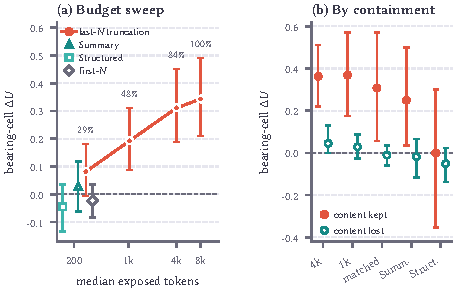
\includegraphics[width=\columnwidth]{fig_lenctl}
\caption{Length-control run on LongMemEval-V2: $\Delta U$ on the
$\lcBearCells$ bearing cells, task-clustered 95\% intervals.
\textbf{(a)}~Raw truncated to its last 4,096 and 1,024 tokens and to each
cell's Summary length (line), against Summary, Structured and the first-$N$
window at that length; percentages give the share of cells whose text still
contains the bearing content. \textbf{(b)}~The same arms split by whether
their text kept the bearing content (filled) or lost it (hollow).}
\label{fig:lenctl}
\Description{Left: bearing-cell utility rising with exposed tokens from about 0.08 at 280 tokens to 0.34 at 8,000, with Summary, Structured and first-N near zero. Right: for each arm, utility near 0.25 to 0.37 when the bearing content is kept and near zero when it is lost, except Structured whose kept estimate is near zero with a wide interval.}
\end{figure}

The length control was frozen before execution. Its extractive arm keeps the
final $N$ tokens of the same source segment, with $N$ set per cell to that
cell's own Summary token count, so it matches Summary's budget without any
model choosing content; a second arm keeps the first $N$ tokens instead, and
last-$N$ versus first-$N$ was registered as the decisive contrast. All three
pre-registered contrasts are computed on the $\lcBearCells$ bearing cells
(two replicate rows each, $\lcPrimaryN$ rows) and clustered over
$\lcBearTasks$ tasks: extractive versus Summary ($\lcPrimary$
$[\lcPrimaryLo, \lcPrimaryHi]$), Raw versus matched extractive ($\lcBudget$
$[\lcBudgetLo, \lcBudgetHi]$), and last-$N$ versus first-$N$ ($\lcEnds$
$[\lcEndsLo, \lcEndsHi]$).

The same run truncated Raw to its last 4,096, 1,024 and 20,000 tokens; the last
equals Raw, since no segment is longer. Table~\ref{tab:sweep} gives each arm's
bearing-cell $\Delta U$, its retention of the bearing content, and $\Delta U$
split by retention. \texttt{make\_lenctl.py} computes every entry from the row
file, whose checksum it verifies against the run manifest, and first checks
that it reproduces the three pre-registered contrasts. The run is not strictly
one session: $\lfLcCacheHits$ responses came from a cache filled minutes
earlier, and $\lcNullRows$ rows with a null reward are excluded, never zeroed.

\begin{table}[t]
\centering\footnotesize
\setlength{\tabcolsep}{2.4pt}
\caption{Length-control run on LongMemEval-V2: bearing-cell $\Delta U$ by arm
($\lcBearCells$ cells, task-clustered 95\% intervals), share of cells whose text
still contains the bearing content, and $\Delta U$ split by whether it does.
Exploratory beyond the three pre-registered contrasts.}
\label{tab:sweep}
\begin{tabular}{@{}lrrrrr@{}}
\toprule
arm & median tokens & kept & $\Delta U$ & $\Delta U\mid$kept & $\Delta U\mid$lost \\
\midrule
Raw (full) & \lcRawTok & \lcRawKept\% & \lcRawM\ [\lcRawLo, \lcRawHi] & \lcRawKM & -- \\
last 4,096 & \lcFourTok & \lcFourKept\% & \lcFourM\ [\lcFourLo, \lcFourHi] & \lcFourKM & \lcFourLM \\
last 1,024 & \lcOneTok & \lcOneKept\% & \lcOneM\ [\lcOneLo, \lcOneHi] & \lcOneKM & \lcOneLM \\
last $N$ (matched) & \lcMatchTok & \lcMatchKept\% & \lcMatchM\ [\lcMatchLo, \lcMatchHi] & \lcMatchKM & \lcMatchLM \\
Summary & \lcSumTok & \lcSumKept\% & \lcSumM\ [\lcSumLo, \lcSumHi] & \lcSumKM & \lcSumLM \\
Structured & \lcStrTok & \lcStrKept\% & \lcStrM\ [\lcStrLo, \lcStrHi] & \lcStrKM & \lcStrLM \\
first $N$ (matched) & \lcFirstTok & \lcFirstKept\% & \lcFirstM\ [\lcFirstLo, \lcFirstHi] & -- & \lcFirstLM \\
\bottomrule
\end{tabular}
\end{table}

\paragraph{Is the kept subset easier?} Retention is a property of the text,
fixed before any outcome, but the cells where a compressed text keeps the
content could still be easier ones. They are not for Summary or the matched
truncation: on the same cells, Raw gains $\lcSelSumKept$ where Summary kept the
content and $\lcSelSumLost$ where it lost it ($\lcSelMatchKept$ and
$\lcSelMatchLost$ for the matched truncation). For Structured the kept cells are
\emph{harder} ($\lcSelStrKept$ against $\lcSelStrLost$), which accounts for
its low kept estimate.

\paragraph{Position.} Target position is identical across all eight arms
within each cell (asserted). Between strata its distribution differs mildly
($\chi^2$ $p = \lcPosChiP$); the position-standardized Raw
\textsc{bearing}$-$control contrast is $\lcPosStd$ against $\lcPosUnadj$
unadjusted, and positive at every position.

\subsection{Formation-cost sensitivity}
\label{sec:reuse}
Formation cost per cell is the writer's tokens divided by the reuse factor
$r$, the number of cells that share one written memory. Our design fixes
$r = \frReuse$, so we recompute exposure efficiency over $r$ from the same
utilities and token counts (Figure~\ref{fig:reuse}). One Summary costs about
$\raFormSum$ writer tokens and one Structured record about $\raFormStr$. On
point estimates Summary overtakes Raw only for $r \gtrsim \raReuseStar$, but
its utility interval spans zero at every $r$, so the crossing point is not
estimated with any precision. Under the sparsity we measure, a memory that
bears on one task may be shown for few others, which pushes $r$ down and
formation cost up. The relevant factor in deployment is exposures per write,
not cells per memory. Input and output tokens are priced identically and prompt
caching is ignored; since output tokens usually cost more, both choices
understate the writer's cost.

\begin{figure}[t]
\centering
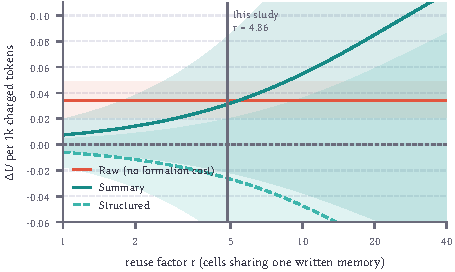
\includegraphics[width=\columnwidth]{fig_reuse}
\caption{Exposure efficiency ($\Delta U$ per thousand charged tokens) against
the reuse factor, on the $\frCells$ representation cells of LongMemEval-V2.
Lines use each representation's paired \textsc{bearing}$-$control effect;
bands use its 95\% interval over memories. Raw has no writer call and does not
depend on $r$. The vertical line marks the reuse factor of this study.}
\label{fig:reuse}
\Description{Line chart of efficiency against reuse factor on a log axis: Raw is flat near 0.034, Summary rises and crosses Raw near r of 5.5 with a wide band spanning zero, Structured is below zero.}
\end{figure}

\section{Second reader and writer, $\times$, reader factorial}
\label{sec:readerfull}

\paragraph{Design.}
The second-reader study was pre-registered before any design-cell call was
issued, with no transfer, the same ordering at a different magnitude, and a
different representation preference all committed as valid outcomes. The
memory file, prompt, filler pool, every rendered request, and each cell's
target position were hash-asserted against the first run at call time, and
the text re-verified byte-identical on $\rgRows$ rows; in the session-matched
run all $\smIdentK$ of $\smIdentN$ joinable rows are hash-identical.

\paragraph{Session-matched result.}
Both readers ran in one session. Over $\rgSmCells$ matched Raw cells on
$\rgSmTasks$ tasks ($\rgSmN$ replicate rows; these three counts are different
units), mean $\Delta U$ is $\rgSmOss$ under the first reader and $\rgSmGem$
under the second, a paired change of $\rgSmDiff$ $[\rgSmLo, \rgSmHi]$. The
two readers' own 95\% intervals overlap; plotting those would invite a ``no
difference'' reading that the paired design rules out. The within-memory
\textsc{bearing}$-$control contrast is $\rgBmcRawOss$ $[\rgBmcRawOssLo,
\rgBmcRawOssHi]$ under the first reader and $\rgBmcRawGem$ $[\rgBmcRawGemLo,
\rgBmcRawGemHi]$ under the second ($\rgBmcRawOssMem$ memories). The no-memory
arm moves by $\rgWithoutDelta$, so part of the gain is a weaker reader rather
than a better memory.

\paragraph{Cross-session first execution.}
A first execution with the two readers a day apart returned $\rgRawDiff$
$[\rgRawLo, \rgRawHi]$, inside the session-matched interval. Re-run together,
that difference splits into $-0.0327$ attributable to the session and
$-0.0364$ to the reader, which halves the apparent reader share. We quote only
the session-matched estimate.

\paragraph{Cell-level agreement, session-matched run.}
These are the numbers behind Figure~\ref{fig:overview}f. Over the
$\rgSmCells$ matched Raw cells, the readers' three-way labels (helped,
unchanged, hurt) agree on $\raReaderLabAgree$ of $\rgSmCells$ cells, at Cohen's
$\kappa = \raReaderKappa$; $\smCZeroZero$ cells are unchanged under both and
can only agree. Of the $\raReaderMoving$ cells that move under either reader,
both mark $\smAgree$ as helped, and signs agree on $\smAgree$ of the $\smBoth$
cells that move under both. The readers agree on no harmed cell (the first
reader's $\raHurtOss$ and the second's $\raHurtGem$ do not overlap), but so few cells
are harmed that this cannot show whether harm labels reproduce.

\paragraph{Cell-level agreement, earlier cross-session run.}
The first execution, with the two readers a day apart, covers a slightly
different matched set ($\rgRawN$ cells) and is the only source for Summary and
Structured. There the readers' per-cell $\Delta U$ correlate at
$r{=}\rgRawRAll$ over all cells, of which $\rgRawZeroBoth$ are zero under both;
over the $\rgRawNNz$ cells non-zero under either reader, $r = \rgRawRNz$
($\rgSumRNz$ for Summary, $\rgStrRNz$ for Structured). Signs agree on
$\rgRawSignK$ of $\rgRawSignN$ Raw cells where both move, and labels on
$\rgRawLabK$ of $\rgRawLabN$. Summary $\rgSumDiff$ $[\rgSumLo, \rgSumHi]$ and
Structured $\rgStrDiff$ $[\rgStrLo, \rgStrHi]$ span zero with only
$\rgSumNNz$ and $\rgStrNNz$ cells non-zero under either reader. Because this
run spans sessions, its numbers mix reader and session differences, and they
should not be pooled with the session-matched ones. Costs are not pooled
across readers: the second reports no reasoning-token counts.

\paragraph{Writer, $\times$, reader factorial.}
\label{sec:factorial}
All four writer--reader arms ran in one session. Every one of the eight
contrasts (writer, reader, same-family and interaction, on Summary with
$n{=}274$ and Structured with $n{=}268$) spans zero. The intervals are
informative rather than underpowered: they exclude writer and same-family
effects larger than $0.0380$, against the $\rgSmDiff$ reader effect the same
apparatus detects. Raw has no writer and is not in the factorial, and two
checkpoints form a $2\times2$ design, not a population of models.

\section{Cross-benchmark contrasts}
\label{sec:crossbenchtable}
The one quantity all three benchmarks define identically is the per-cell
representation contrast: a representation's $\Delta U$ minus Raw's on the same
memory and task. It separates from zero on LongMemEval-V2 alone
(Figure~\ref{fig:overview}e): Summary$-$Raw is $\xbSRLmM$
$[\xbSRLmLo, \xbSRLmHi]$ and Structured$-$Raw is $\xbTRLmM$
$[\xbTRLmLo, \xbTRLmHi]$ on $\xbSRLmN$ cells. On SciCode ($n{=}\xbSRScN$) and
SWE-bench Verified ($n{=}\xbSRSwN$) every interval includes zero, but there the
memories themselves have no effect even in raw form: Raw's own $\Delta U$ is
$\rvSciRaw$ $[\rvSciRawLo, \rvSciRawHi]$ on SciCode, where $\rvSciRawTied$ of
$\rvSciRawN$ cells are unchanged, and $\rvSweRaw$ $[\rvSweRawLo, \rvSweRawHi]$
on SWE-bench. With no Raw effect to preserve or lose, a representation contrast
there is uninformative about representation; these benchmarks bound where
memory matters for this reader, not how it should be written
(Section~\ref{sec:crossbenchtable}).

Table~\ref{tab:crossbench} gives the values plotted in
Figure~\ref{fig:overview}e. We compare contrasts rather than
per-representation $\Delta U$ because each benchmark carries its own
nondeterminism. The no-memory arm, whose input is identical across
representations, still disagrees with itself on
$\xbFloorLmK/\xbFloorLmN{=}\xbFloorLm$ of LongMemEval-V2 cells and
$\xbFloorScK/\xbFloorScN{=}\xbFloorSc$ of SciCode cells, and a paired contrast
removes that term. SWE-bench has no such floor because its no-memory arm is
deterministic by construction. SciCode's equivalent judge control disagrees
on 5 of 135 cells within one session, so determinism cannot be assumed of a
new benchmark.

\begin{table}[t]
\centering\footnotesize
\setlength{\tabcolsep}{4pt}
\caption{Per-cell representation contrasts: $\Delta U$ under one
representation minus $\Delta U$ under Raw on the same memory and task, with
task-clustered 95\% intervals. Only LongMemEval-V2 separates from zero. Every
SciCode and SWE-bench interval includes zero (SWE-bench's Summary$-$Raw only at
its upper bound), and doubling the SciCode cell
count separated no contrast. MDE is the minimum detectable contrast at 80\%
power and two-sided $\alpha = 0.05$, computed from each interval's width.
Raw's own with-versus-without $\Delta U$ is $\rvSciRaw$
$[\rvSciRawLo, \rvSciRawHi]$ on SciCode and $\rvSweRaw$ on SWE-bench, so on
these benchmarks no memory effect exists for a representation to preserve, and
the contrasts cannot test the ordering.}
\label{tab:crossbench}
\setlength{\tabcolsep}{3pt}
\begin{tabular}{@{}llrrrr@{}}
\toprule
contrast & benchmark & $n$ & mean & 95\% CI & MDE \\
\midrule
Summary$-$Raw
 & LongMemEval-V2 & \xbSRLmN & \xbSRLmM & [\xbSRLmLo, \xbSRLmHi] & \raMdeSRLm \\
 & SciCode        & \xbSRScN & \xbSRScM & [\xbSRScLo, \xbSRScHi] & \raMdeSRSc \\
 & SWE-bench      & \xbSRSwN & \xbSRSwM & [\xbSRSwLo, \xbSRSwHi] & \raMdeSRSw \\
\midrule
Structured$-$Raw
 & LongMemEval-V2 & \xbTRLmN & \xbTRLmM & [\xbTRLmLo, \xbTRLmHi] & \raMdeTRLm \\
 & SciCode        & \xbTRScN & \xbTRScM & [\xbTRScLo, \xbTRScHi] & \raMdeTRSc \\
 & SWE-bench      & \xbTRSwN & \xbTRSwM & [\xbTRSwLo, \xbTRSwHi] & \raMdeTRSw \\
\bottomrule
\end{tabular}
\end{table}

\section{Sign reversal and the decomposition}
\label{sec:negative}
\paragraph{Why flip rates cannot be compared across strata.}
A memory can show a flip only if at least two of its cells move with opposite
signs, so the chance of a flip grows with the number of cells per memory. In
the screened design a memory has $\raCellsPerMemBear$ \textsc{bearing} cells
and $\raCellsPerMemRand$ \textsc{random} cells on average. The naive
contrast (0 of 35 \textsc{bearing} memories against 17 of 60 \textsc{random},
Fisher one-sided $p = 1.5\times10^{-4}$) therefore mostly reflects that
difference. To test this, we took each of the $\raMatchedN$ memories with at
least two \textsc{bearing} cells and drew, without replacement, as many of its
\textsc{random} cells as it has \textsc{bearing} cells, then recounted flips
(20{,}000 resamples). The random stratum averages $\raMatchedMean$ flips and
shows none in $\raMatchedPZero\%$ of resamples (Figure~\ref{fig:reversal}b), so
0 of 35 is what chance alone would most often produce. A Wilson bound on the \textsc{bearing} flip rate would also treat 35 memories
from 21 episodes as independent.
Matching each memory's random subsample on the no-memory outcome as well (so
both strata get the same opportunities to help and to hurt) leaves all
$\lfCondFlipMems$ memories eligible; the random stratum then shows a mean of
$\lfCondFlipMean$ flips and none in $\lfCondFlipPZero\%$ of resamples. We
therefore do not compare flip rates across strata.

\paragraph{Why the sign of moving cells is not a comparison either.}
A tempting alternative compares the share of negative cells among cells that
move: $\raNegBearK$ of $\raNegBearN$ for \textsc{bearing} against
$\raNegRandK$ of $\raNegRandN$ for \textsc{random}. That comparison is
confounded by baseline accuracy. A memory can only hurt where the reader was
correct without it, and \textsc{bearing} tasks have the lowest no-memory
accuracy, so they offer the fewest chances to hurt.

\paragraph{Transitions conditioned on the no-memory outcome.}
Reward is binary in the screened run: each stratum's mean equals
(helped $-$ hurt)$/n$ exactly. With Table~\ref*{M-tab:screened}'s both-arms-fail
rate this fixes the full transition table (Table~\ref{tab:transitions}).
Conditioned on opportunity, the strata do not differ detectably in harm,
and they differ sharply in help (Figure~\ref{fig:reversal}a). In the
\textsc{random} stratum help and harm rates are close, the signature of a
content-independent response to inserting an item, which we treat as the
perturbation floor (\main{sec:metrics}). The table's Wilson intervals treat cells as
independent. Resampling memories instead, the harm rates have intervals of
$[\lfHurtClBearLo, \lfHurtClBearHi]$ (\textsc{bearing}),
$[\lfHurtClCtrlLo, \lfHurtClCtrlHi]$ (control) and
$[\lfHurtClRandLo, \lfHurtClRandHi]$ (\textsc{random}), which overlap, and the
help rates $[\lfHelpClBearLo, \lfHelpClBearHi]$,
$[\lfHelpClCtrlLo, \lfHelpClCtrlHi]$ and $[\lfHelpClRandLo, \lfHelpClRandHi]$,
where \textsc{bearing}'s is disjoint from the others. Both
analyses here are exploratory and are produced by
\texttt{make\_reanalysis.py}, which first checks that it reproduces every flip
count and stratum mean in the paper.

\begin{table}[t]
\centering\footnotesize
\setlength{\tabcolsep}{2.6pt}
\caption{Screened run on LongMemEval-V2: transitions between the no-memory
and with-memory outcome (binary reward). Accuracy columns give the share of
cells answered correctly without and with the memory. Hurt is conditioned on
cells correct without the memory, help on cells wrong without it; Wilson 95\%
intervals in brackets.}
\label{tab:transitions}
\begin{tabular}{@{}lrrrrr@{}}
\toprule
stratum & $n$ & acc.\ w/o & acc.\ with & hurt $\mid$ correct & help $\mid$ wrong \\
\midrule
\textsc{bearing} & \spBearN & \raAccZeroBear & \raAccOneBear
  & \raHurtRateBear\ [\raHurtLoBear, \raHurtHiBear] & \raHelpRateBear\ [\raHelpLoBear, \raHelpHiBear] \\
control & \spCtrlN & \raAccZeroCtrl & \raAccOneCtrl
  & \raHurtRateCtrl\ [\raHurtLoCtrl, \raHurtHiCtrl] & \raHelpRateCtrl\ [\raHelpLoCtrl, \raHelpHiCtrl] \\
\textsc{random} & \spRandN & \raAccZeroRand & \raAccOneRand
  & \raHurtRateRand\ [\raHurtLoRand, \raHurtHiRand] & \raHelpRateRand\ [\raHelpLoRand, \raHelpHiRand] \\
\midrule
\multicolumn{6}{@{}l}{\emph{opportunities:} hurt $\raHurtOppBear$ / $\raHurtOppCtrl$ / $\raHurtOppRand$ cells;
help $\raHelpOppBear$ / $\raHelpOppCtrl$ / $\raHelpOppRand$ cells} \\
\bottomrule
\end{tabular}
\end{table}

\paragraph{The additive-null comparison.}
Fitting $\mu + a_m + b_t$ and simulating from it, the excess of the observed
reversal rate over the fitted additive model is negative in all three strata.
Two independent implementations agree on the sign and disagree on the
magnitude, so we quote only the sign.

\paragraph{Why the decomposition is not identifiable.}
The within-session execution floor is exactly zero: replicates issued 0--16
seconds apart agree on 1{,}157 of 1{,}157 cells. With no residual scale, the
fitted residual collapses and the task and interaction shares are not
separately identified, so we report none. Clean per-cell utilities and a
variance decomposition are in tension on a reader without execution noise.

\begin{figure}[t]
\centering
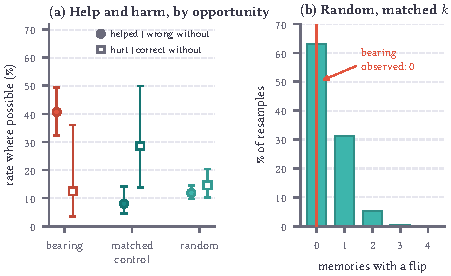
\includegraphics[width=\columnwidth]{fig_reversal}
\caption{Sign reversal on LongMemEval-V2, screened design (1{,}157 cells,
60 memories). \textbf{(a)}~Help rate among cells the reader got wrong without
the memory (filled) and harm rate among cells it got right (hollow), with
Wilson 95\% intervals; counts are in Table~\ref{tab:transitions}. Harm does not differ detectably across
strata; help does. \textbf{(b)}~Flips among the 35 memories with at least two
\textsc{bearing} cells when each memory's \textsc{random} cells are subsampled
to its own \textsc{bearing}-cell count (20{,}000 resamples); the line marks the
observed \textsc{bearing} count.}
\label{fig:reversal}
\Description{Left: dot plot of help and harm rates by stratum; help is about 41 percent for bearing against 8 and 12 percent elsewhere, harm overlaps across strata at 12 to 29 percent with wide intervals. Right: histogram of flip counts at matched cell counts, with zero flips in about 63 percent of resamples.}
\end{figure}

\section{Data, code and prompt availability}
\label{sec:repro}
\label{sec:prompts}
\paragraph{Public dataset.} The Conditional Memory Utility Dataset is available on
\href{https://huggingface.co/datasets/AgentsSci/AAMAS2027-ConditionalMemory}{Hugging Face}.
The frozen \texttt{v0.6-}\allowbreak\texttt{length-control} snapshot contains 16,816 records:
16,535 from LongMemEval-V2, 154 from SciCode, and 127 from SWE-bench Verified.
A row describes a memory--task pair under a representation, reader, condition
and replicate, with the outcome under each arm, available output text and
cost metadata. Missing or unscorable measurements remain explicitly marked;
they must not be converted to zero rewards.

\paragraph{Version and reproducibility.} The data file is
\texttt{data/}\allowbreak\texttt{cells.jsonl}. The repository also provides a manifest with file checksums, schema and validation
code, and documentation of the included conditions and upstream sources.
Readers can download the data directly or pin the
\texttt{v0.6-}\allowbreak\texttt{length-control} revision with the Hugging Face client. The data
card contains a runnable download example and explains the validation warnings.
This snapshot was built on 2 October 2026 and does not contain every later
manuscript analysis; in particular, its condition inventory does not include
the fixed-total-context experiment. The public Hub package contains schema and
validation code, not the complete experiment, analysis and prompt bundle.
The length-control identity arm is an A/A control and must not be pooled with
Raw as an independent condition. Per-pair utility labels describe the recorded
evaluation conditions, rather than unconditional training targets.

\paragraph{Withheld and missing text.} The 154 SciCode records contain Raw
memories; their reader outputs were not retained. SciCode Summary and Structured
records are absent because their memory text was not persisted. The 127
SWE-bench records provide identifiers and derived measurements, with restricted
corpus and output text withheld under the release policy. These are distinct
from records missing because of a persistence gap. The data card documents the
sentinels and per-source reuse terms; access to the dataset does not grant a
new license to withheld upstream content.

\section{Extended limitations}
\label{sec:extlimits}

\paragraph{Leakage rates are lower bounds.}
Our leakage detector reuses the benchmark's phrase matcher, whose normalizer
strips punctuation without inserting a space. A gold phrase next to a quote
or an equals sign is glued to its neighbor and the match fails. Such leaks
are missed, and punctuation is common in accessibility trees, so every
leakage rate we report is a lower bound. A control test records the defect, so
an upstream fix would be detected. The 156
LLM-judged questions cannot be audited without an inference call and are
recorded as undecidable rather than clean. 69 multiple-choice questions with
gold answers of one to five characters cannot be audited structurally and are
never folded into a pooled rate.

\paragraph{The judge floor measures decoding.}
$F_{\mathrm{judge}}$ is zero wherever we measured it: over $\lfJudgeObs$
explicit re-scorings of $\lfJudgeUnits$ units in the earlier official arm, and
in every stratum of the screened run. Both estimators carry a positive control
(a planted disagreement makes them fire). A zero floor here reflects a
deterministic scorer and greedy decoding, not an unambiguous rubric. The
SciCode control in Section~\ref{sec:crossbenchtable}, which disagrees on 5 of
135 cells, is a different scorer on a different benchmark. We have no
cross-session floor for any arm and presume it to be non-zero.
%%% NOTE: earlier drafts quoted "240 of 240" and "288 re-scorings"; neither
%%% figure could be traced to a ledger in results/, so both were replaced.

\paragraph{Semantic type.}
We intended semantic memory type as a second axis, but in our representation
pilot the two labeling passes agreed on 3 of 8 segments at Cohen's
$\kappa = 0.000$: the structured writer's own pass called every segment
\texttt{episodic}, a degenerate marginal, so we report no semantic-type
breakdown. Separately, exactly one deterministically scorable
\emph{errors-gotchas} question exists in the benchmark and accounts for 865 of
6{,}920 web cells, so any per-stratum result there is a single-question result.

\paragraph{Writer failures and faithfulness.}
The structured writer failed on 3 of 60 segments, all by exhausting the token
budget mid-value rather than by malformed output, and on 0 of the 57 writes
that finished. An 8-segment pilot had put the failure rate at 0 of 8 and could
not have seen this, since it never reached the cap. Our faithfulness measures
are a screen, not a guarantee: a low score is strong evidence of a problem,
a high score is weak evidence of its absence, and they do not detect
recombination, omission, unsupported inference or negation.

\paragraph{Unrecorded quantities.}
Two quantities were not recorded during the runs and cannot be recovered: how
many gold-free picks contain the answer, and how the 12 position-probe cells
were chosen, which is why we treat that probe as a pilot.

\paragraph{Stated exclusions.}
17 of the 295 deterministically scored questions have no memory unit that
carries their gold answer under the segmentation answerability check, so their
cells can only yield $\Delta U \le 0$. The bearing screen, a looser containment
test, fires on no unit for $\soScrZero$ of them (Section~\ref{sec:sophia}).
23 of the 1{,}889 units (1.2\%) are their entire trajectory.

\section{Pre-registration record}
\label{sec:prereg}
Each pre-registered analysis was fixed in a pre-commitment document in the code
repository before the data it governs existed. The documents are released with
the code. To preserve anonymity we omit their commit identifiers here; the
release links each one to a commit and its timestamp, so its timing can be
checked on de-anonymization. Table~\ref{tab:prereg} lists every pre-registered analysis, its
anchor, and every deviation the run ledgers record. Pre-commitments were not edited after
the fact; where a result does not match one, the mismatch is reported.

\begin{table}[h]
\centering\footnotesize
\setlength{\tabcolsep}{3pt}
\caption{Pre-registered analyses, their anchors, and recorded deviations.}
\label{tab:prereg}
\begin{tabular}{@{}p{0.27\columnwidth}p{0.30\columnwidth}p{0.37\columnwidth}@{}}
\toprule
analysis & anchor & recorded deviation \\
\midrule
screened design and its reduction criterion & criterion fixed in code before the numbers existed & none recorded \\
reversal rate (headline) & pre-registration, section~5 & comparison with an additive null added later, as a diagnostic \\
variance decomposition & pre-registration, section~6 & not identifiable here (zero execution floor); in earlier arms the mixed model did not converge and the registered fallback was used \\
gold-free screens & gold-free screen pre-commitment & none recorded \\
length control & frozen at a recorded commit, before execution & \lfPrLcMismatch\ of \lfPrLcCompared\ descriptive figures do not re-derive: bearing quartile means by Raw length; none appears in the paper \\
second reader & written before any design-cell call & cross-session estimate superseded by a session-matched run \\
session-matched reader run & falsifiers committed before data & none recorded \\
writer\,$\times$\,reader factorial & factorial pre-commitment & one prose sign error ($-\tfrac12$ for $+\tfrac12$ interaction); replication check fails on sign only \\
SciCode scale-up & scale-up pre-commitment & none recorded \\
\bottomrule
\end{tabular}
\end{table}

\paragraph{The two deviations that bear on results.} The additive-null
comparison of reversal rates (\main{sec:r0}) was \emph{not} pre-registered;
the registered headline is the reversal rate itself, and the comparison is a
diagnostic added afterwards. In the writer\,$\times$\,reader factorial, the
registered criterion asked the re-measured reader effect to reproduce the
earlier one in sign and significance. Both estimates are near zero and span
zero (Summary $\lfPrWfSumOld$ then $\lfPrWfSumNew$, Structured
$\lfPrWfStrOld$ then $\lfPrWfStrNew$), so the significance verdict reproduces
and the sign does not; the two intervals contain each other's point estimates.
The factorial's pre-commitment also states that the same-family effect equals
$-\tfrac12$ of the interaction; the correct relation, which the analysis code
checks numerically, is $+\tfrac12$. Every quantity was computed as registered.

\section{Follow-up runs}
\label{sec:sophia}
Three follow-up runs test the main results under conditions the main design
held fixed; all are exploratory and used the same serving endpoint and reader as
the main runs. A generator script in the released code computes every number
below from the row files.

\paragraph{Second session, randomized position.} All $\soXoneCells$ bearing and
control cells, three replicates each, the memory's position redrawn per
replicate ($\soXoneCalls$ real calls, $\soXoneCacheHits$ from cache,
$\soXoneErr$ failed and excluded). Bearing minus control, paired within memory:
$\soXoneD$ $[\soXoneLo, \soXoneHi]$ over $\soXoneMems$ memories;
episode-clustered $[\soXoneEpLo, \soXoneEpHi]$ ($\soXoneEps$ episodes); two-way
(memory $\times$ task) $\soXoneTw$ $[\soXoneTwLo, \soXoneTwHi]$. Across the
three positions of a cell, the label changes in $\soPosChg$ of $\soPosCells$
cells ($\soPosChgPct\%$), and in $\soPosChgMv$ of the $\soPosMov$ cells that move
at least once ($\soPosChgMvPct\%$); position accounts for $\soPosVarPct\%$ of
the variance of $\Delta U$. Joined one-to-one to the published run, labels agree
in $\soStabSamePct\%$ of $\soStabSameN$ replicate-cells at the same position
($\kappa = \soStabSameK$) and in $\soStabDiffPct\%$ of $\soStabDiffN$ at a new
one ($\kappa = \soStabDiffK$).

\paragraph{Fixed total context.} $\soXtwoCells$ cells over $\soXtwoMems$
memories, two replicates. For each cell, $T$ is the base filler plus the Raw
memory; every other arm, and the no-memory arm, is padded after the base context
with bearing-disjoint filler to $T$ (asserted equal across arms), the memory
kept at its K2 position. \emph{Disclosed defect:} the no-memory cache key was
(trajectory, task, replicate), so two memories from one trajectory paired with
one task could share a no-memory response although their padding differs. The
headline numbers exclude all $\soXtwoCollCells$ such cells ($n=\soFN$ bearing
cells); including them ($n=\soFNAll$) changes no conclusion:

\begin{table}[!ht]
\centering\footnotesize
\setlength{\tabcolsep}{3pt}
\caption{Bearing-cell $\Delta U$ at a fixed total context (task-clustered
95\% intervals).}
\label{tab:fixedctx}
\begin{tabular}{@{}lll@{}}
\toprule
arm & excluding exposed cells & all cells \\
\midrule
Raw & \soFRaw\ [\soFRawLo, \soFRawHi] & \soFRawAll\ [\soFRawAllLo, \soFRawAllHi] \\
Summary & \soFSum\ [\soFSumLo, \soFSumHi] & \soFSumAll\ [\soFSumAllLo, \soFSumAllHi] \\
Structured & \soFStr\ [\soFStrLo, \soFStrHi] & \soFStrAll\ [\soFStrAllLo, \soFStrAllHi] \\
matched truncation & \soFTr\ [\soFTrLo, \soFTrHi] & \soFTrAll\ [\soFTrAllLo, \soFTrAllHi] \\
Summary $-$ Raw & \soFSumR\ [\soFSumRLo, \soFSumRHi] & \soFSumRAll\ [\soFSumRAllLo, \soFSumRAllHi] \\
Structured $-$ Raw & \soFStrR\ [\soFStrRLo, \soFStrRHi] & \soFStrRAll\ [\soFStrRAllLo, \soFStrRAllHi] \\
\bottomrule
\end{tabular}
\end{table}

The matched truncation is sensitive to the exclusion and supports no claim. The
cache key now includes the memory, so a re-run cannot repeat the defect.

\paragraph{Retrieval.} The reference labels are the screened design's (75 tasks, 266
bearing edges, reproduced and asserted). Each method ranks the task's whole
domain pool by the raw question; dense retrieval embeds 512-token chunks (a
unit scores its best chunk) or the first 2{,}000 tokens.

\begin{table}[!ht]
\centering\footnotesize
\setlength{\tabcolsep}{3pt}
\caption{Retrieval of bearing units (task-clustered 95\% intervals; chance
recall@10 is about \soChanceTenP). MRR is the mean reciprocal rank of the first
bearing unit; AUROC is the area under the ROC curve over bearing and
non-bearing units.}
\label{tab:retrieval}
\begin{tabular}{@{}lllll@{}}
\toprule
method & recall@1 & recall@10 & MRR & AUROC \\
\midrule
BM25 & \soRBmOne & \soRBmTen\ [\soRBmTenLo, \soRBmTenHi] & \soRBmMrr & \soRBmAuc \\
dense, prefix & \soRPreOne & \soRPreTen\ [\soRPreTenLo, \soRPreTenHi] & \soRPreMrr & \soRPreAuc \\
dense, chunks & \soRChkOne & \soRChkTen\ [\soRChkTenLo, \soRChkTenHi] & \soRChkMrr & \soRChkAuc \\
\bottomrule
\end{tabular}
\end{table}

Of the 295 deterministic questions, $\soScrZero$ fire on no unit, $\soScrDisc$
on one to eight, and $\soScrOver$ on more than eight. Without the cap, string
containment fires for all $\soNoCapMems$ memories, on $\soNoCapMin$ to
$\soNoCapMax$ tasks each.

\paragraph{Variance decomposition.} In the second-session run each cell has three
replicates at redrawn positions, which supplies the residual scale the main run
lacked. On the $\rvDecCells$ cells with all three replicates we fit the additive
model $\mu + a_m + b_t$ to cell means by least squares; its residual mean square
($\rvDecDf$ degrees of freedom) estimates the interaction variance plus the
within-cell variance divided by three, and the within-cell variance estimates the
residual. The shares are $\rvIntShare\%$ interaction, $\rvAddShare\%$ additive
memory and task effects, and $\rvEpsShare\%$ position with decoding; the
interaction $F$ test gives $F=\rvIntF$ ($p\rvIntP$). This is a method-of-moments
estimate on a sparse crossed design, reported as exploratory.

\paragraph{Power for harm.} With $16$ bearing cells able to show harm, against
the random stratum's rate of $\rvHarmRandPct\%$, the screened design detects
(80\% power, two-sided $\alpha=0.05$) only a bearing harm rate of
$\rvHarmMdePct\%$ or more; the null on harm is therefore weak evidence.

\paragraph{Containment inside the random-task stratum.} Memories in this stratum are real
same-domain pages. On the $\rvRandFireN$ random cells where the containment
detector fires (at any breadth) the memory helps in $\rvRandFireHelp\%$ of the
$\rvRandFireHelpN$ cells the reader got wrong without it, against
$\rvRandSilentHelp\%$ of $\rvRandSilentHelpN$ where it is silent; harm is
$\rvRandFireHurt\%$ and $\rvRandSilentHurt\%$. Part of the random stratum's help
is content, so its help rate bounds pure perturbation from above.

\paragraph{The gold-free screen over the full universe.} The model-based screen
was applied to all $\rvGfUniverse$ (task, unit) pairs: an exhaustive lexical
stage kept $\rvGfCand$ candidates, and the judge confirmed $\rvGfYes$ over
$\rvGfTasks$ tasks and $\rvGfMems$ memories, under the same cap of eight units
per task. A gold-free definition does not make bearing denser.

\paragraph{Sparsity across screen caps.} Recomputing the screen over the
deterministic tasks at four caps on the number of units a task may fire on:
at a cap of 4, $\rvCapFourTasks$ tasks and $\rvCapFourMems$ bearing memories;
at 8 (the paper's screen), $\rvCapEightTasks$ and $\rvCapEightMems$; at 16,
$\rvCapSixteenTasks$ and $\rvCapSixteenMems$; at 32, $\rvCapThirtyTwoTasks$ and
$\rvCapThirtyTwoMems$. At every cap the median bearing memory bears on exactly one
task, and $\rvCapShareLo$--$\rvCapShareHi\%$ bear on exactly one. Only removing the
cap entirely makes containment fire for every memory.

\paragraph{Which memories were sampled.} The 60 memories are every memory that
bears on two or more tasks and passes the size cap ($\rvSelMulti$ of the
corpus's $\rvPopMulti$) plus $\rvSelSingle$ single-task memories. The headline
contrast is $\rvHeadSingle$ $[\rvHeadSingleLo, \rvHeadSingleHi]$ on the
single-task memories and $\rvHeadMulti$ $[\rvHeadMultiLo, \rvHeadMultiHi]$ on the
multi-task ones; reweighted to the $\rvPopAll$ bearing memories of the corpus, of
which $\rvPopSinglePct\%$ bear on one task, it is $\rvHeadW$
$[\rvHeadWLo, \rvHeadWHi]$ (memory bootstrap within each group).


\section{Additional figures}
\label{sec:figs}
Figure~\ref{fig:overview} collects views referenced from the main paper: bearing
breadth, helped cells by stratum, retrieval, the representation contrasts with
their token costs, the cross-benchmark contrasts, and the two readers'
agreement. Figure~\ref{fig:lenctl} (Section~\ref{sec:lengthcontrol}) details the
length-control run.



\begin{figure*}[p]
\centering
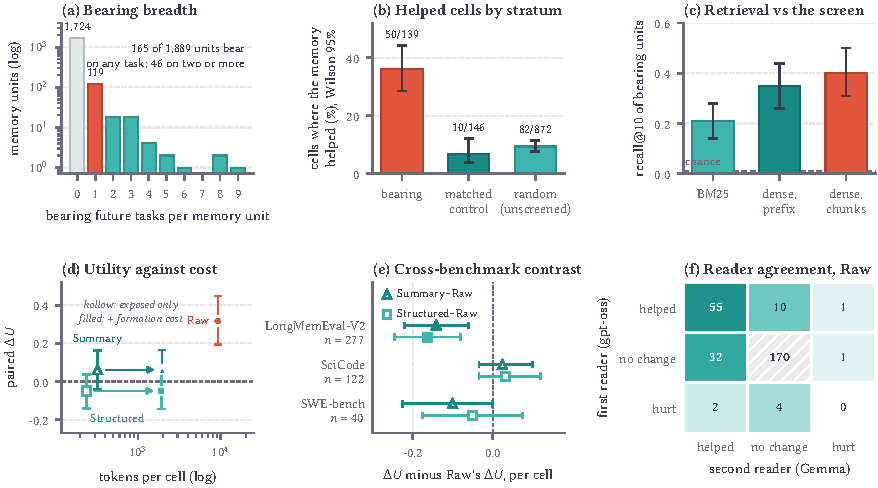
\includegraphics[width=\textwidth]{fig_results}
\caption{Overview of further results on LongMemEval-V2 (a--d, f) and across
benchmarks (e). \textbf{(a)}~Future tasks each of the $\bearUnits$ memory units
bears on, over $\bearDetTasks$ discriminative tasks (log axis).
\textbf{(b)}~Share of cells where the memory helped, cell-level Wilson 95\%
intervals (memory-resampled ones in Section~\ref{sec:negative}), for
the same $\spMems$ memories in three strata. \textbf{(c)}~Share of bearing units a retriever ranks in its top ten of the
domain pool (75 tasks, task-clustered 95\% intervals); the dashed line is
chance. \textbf{(d)}~Paired
\textsc{bearing}$-$control effect per representation ($\frCells$ cells,
$\frMems$ memories, intervals over memories); hollow markers count exposed
tokens, filled ones add formation cost amortized over $\frReuse$ cells.
\textbf{(e)}~Per-cell $\Delta U$ minus Raw's, task-clustered intervals; filled
markers exclude zero. \textbf{(f)}~Two readers' labels on $\rgSmCells$ Raw cells
in one session; the hatched cell (zero under both) cannot disagree.}
\label{fig:overview}
\Description{Six panels: a log histogram of bearing tasks per memory unit peaking at one; bar chart of helped-cell rates by stratum with bearing highest; similarity sextile lines nearly flat; utility against tokens showing Raw above zero and compressed representations near zero; cross-benchmark contrast intervals, only LongMemEval-V2 excluding zero; a three by three reader agreement table.}
\end{figure*}




%%%%%%%%%%%%%%%%%%%%%%%%%%%%%%%%%%%%%%%%%%%%%%%%%%%%%%%%%%%%%%%%%%%%%%%%

\clearpage
\section*{Supplementary Material}
\label{sec:supplementary-material}

% Use S1, S2, ... section numbering and S1, S2, ... figure/table numbering.
% Page numbering continues from the main paper.
\setcounter{section}{0}
\setcounter{subsection}{0}
\setcounter{figure}{0}
\setcounter{table}{0}
\renewcommand{\thesection}{S\arabic{section}}
\renewcommand{\thesubsection}{\thesection.\arabic{subsection}}
\renewcommand{\thefigure}{S\arabic{figure}}
\renewcommand{\thetable}{S\arabic{table}}

% References from the supplement to sections, tables, and figures in main.tex.
\providecommand{\main}[1]{main paper, Section~\ref*{M-#1}}

% Supplementary sections.
\noindent\textbf{Guide to this supplement.}
The paper is self-contained, and this document holds the detail behind it. Section~\ref{sec:protocol} gives the full protocol: how the
writer is kept blind to future tasks, how target position is controlled,
both gold-free screens, and the leakage audit.
Section~\ref{sec:benchdetails} describes the benchmark adapters, the scorer,
pairing and power, and why each secondary benchmark has the yield it has.
Section~\ref{sec:config} lists the frozen execution configuration, the noise
floors, the label definitions, and why the additive null and the variance
decomposition matter. Section~\ref{sec:lmresults} adds LongMemEval-V2
results: the cell-level sparsity map, the reader capability check, the
length-control design, and the formation-cost sensitivity. Section~\ref{sec:readerfull} reports the
second-reader study and the writer-by-reader factorial in full, and
Section~\ref{sec:crossbenchtable} gives the cross-benchmark contrasts as a
table. Section~\ref{sec:negative} reports the sign-reversal analysis the study
was designed around, including why naive sign comparisons mislead and the
transition analysis that replaces them. Section~\ref{sec:repro} covers data, code and
prompt availability, licensing and reproducibility, and
Section~\ref{sec:extlimits} the limitations not needed to read the main result. Section~\ref{sec:prereg} is the pre-registration record: every
pre-registered analysis, its anchor, and every recorded deviation. Section~\ref{sec:sophia} reports three follow-up runs: a second session
with randomized position, a fixed total context, and a retrieval evaluation. Every table and figure states its
benchmark, population and denominator.

\section{Protocol details}
\label{sec:protocol}

\subsection{Keeping the writer blind to future tasks}
\label{sec:taskblind}
Memory formation must be a function of the past episode alone, $m = W(e)$.
If the writer could see a future task, a positive $\Delta U$ would show only
that a model can be told the answer and copy it forward. We enforce this with
four structural barriers rather than by convention. (1)~\emph{Arity}: the
writer function takes a segment and nothing else. (2)~\emph{A closed field
set}: the writer emits only the fields of its schema. (3)~\emph{A metadata
denylist}: the weakest barrier, present to make a plumbing mistake fail loudly.
(4)~\emph{A single interpolation point}: the prompt has one placeholder, the
segment text. Each barrier carries a negative control that plants the defect
and requires the check to fire. Prompt identity is derived from the prompt
file's bytes, not from a hand-maintained version constant that could report a
stale version.

\subsection{Target position is held fixed}
\label{sec:position}
The \textsc{with} arm holds one more item than the \textsc{without} arm, so
some rule must place it, and that rule is not neutral. Holding the memory,
question, filler, model, decoding and seed fixed and varying only the
position of the target memory changes the answer in 8 of 12 probe cells. Measured at scale in the second-session
run (Section~\ref{sec:sophia}), position changes $\soPosChgPct\%$ of labels. A
comparison that does not control position therefore measures position
together with presence. We hold position fixed across replicates, vary it
across cells, and record it on every row. This is also what makes the
second-reader comparison (\main{sec:readertransfer}) a comparison of readers
and not of positions. The probe is small ($n{=}12$), and we treat the rate
as provisional.

\subsection{The bearing screen and both gold-free screens}
\label{sec:goldfree}
The bearing screen reads the memory text, the task's gold answer, and the
task's evaluation specification; it never reads the question. A pair is
\textsc{bearing} only when the benchmark's scorer marks the memory text
correct against the gold answer \emph{and} the test fires on at most eight of
the 865--1{,}024 units in the task's domain pool. The second clause matters.
An earlier, non-discriminative version of the flag fired on nearly every
candidate: its rate on paired versus unpaired memories was in a ratio of
$0.995$, so it said nothing about any one of them.

We pre-registered two gold-free screens before execution. Each reads the
memory, the question and the same-domain pool, and none of the gold answer,
the reward, any model output, or the evaluation specification. We report
both, because reporting only the screen that worked would select an
instrument on its outcome.
\begin{itemize}
\item \emph{Model-based screen.} The judge is $\lfGfJudge$, the reader's own
model, at temperature 0, asked whether the memory contains the specific
information the question asks about. On cells the gold screen never
selected, its picks move the reader from $\gfWithoutPct\%$ correct without the
memory to $\gfWithPct\%$ with it ($\gfN$ rows, $\gfCells$ cells); its matched
control moves from $\gfCtlWithoutPct\%$ to $\gfCtlWithPct\%$ ($\gfCtlN$ rows,
$\lfGfCtlCells$ cells). The contrast of $\gfDiff$ has a task-clustered interval
of $[\lfGfTaskLo, \lfGfTaskHi]$ ($\lfGfTaskN$ tasks), an episode-clustered one
of $[\lfGfEpLo, \lfGfEpHi]$ ($\lfGfEpN$ episodes), and a paired-by-memory
difference of $\lfGfMemD$ over $\lfGfMemN$ memories. Against the gold screen it
recovers $\lfGfBoth$ of $\lfGfGold$ gold-bearing pairs ($\lfGfRec\%$ recall),
and $\lfGfBoth$ of its $\lfGfPicks$ picks are gold-bearing ($\lfGfPrec\%$). The
run is in one session, separate from the gold run.
\item \emph{Lexical screen.} It returns no effect. A diagnostic independent of
any utility explains why: its bearing cells fail in both arms at a rate of
$\gfLexBaf$, \emph{worse} than unscreened random pairing, against
$\gfLlmBaf$ for the model-based screen. A criterion whose selections are
harder than a random draw has not located bearing pairs.
\end{itemize}

\subsection{Leakage audit}
\label{sec:leakage}
The writer invariant excludes \emph{task-directed writing}, not a naturally
occurring memory that happens to contain a later answer. Such a memory is
genuinely useful, and removing it would condition the cell set on the
outcome. We therefore audit every cell rather than filter it. The detector
reuses the benchmark's own scorer and asks whether the rendered memory text
alone would score correct against the gold answer. For \textsc{bearing} cells
the answer is yes by construction, since that is half the bearing definition.
The audit carries information for the control and \textsc{random} strata and
for the Summary and Structured texts, where containment is not guaranteed and
can be conditioned on in analysis. It is validated by 17
controls (plants it must catch, clean cases it must not fire on, and two
pinned known false negatives) and aborts if any control fails.

\subsection{Three kinds of zero in the cost ledger}
\label{sec:zeros}
Raw makes zero writer calls; Summary and Structured make one each per
segment. The ledger distinguishes three zeros that are routinely merged: a
measured zero (Raw makes zero extraction calls), an absent measurement (no
call was made, so the cell leaves that denominator), and an unreported field
(the endpoint exposes no counter). Failed writes count: a write that failed
after consuming a call still cost that call.

\section{Benchmark adapters and coverage}
\label{sec:benchdetails}

\paragraph{LongMemEval-V2 haystacks.}
On the \texttt{small} tier each domain has exactly one haystack, identical
across questions even as an ordered tuple, so every memory is available to
every question in its domain and there is no availability confound between
arms. The same test returns 222 and 211 distinct haystacks on
\texttt{medium}, a positive control showing that it distinguishes the two
cases. Trajectory lengths were measured with the benchmark's own tokenizer
over 200 trajectories and 5{,}095 states.

\paragraph{Scorer dispatch.}
There are eight distinct evaluation-specification strings, not six: two
phrase-match variants differ only in their separator. The adapter therefore
dispatches on the full string, never on the function name, and calls the
benchmark's scorer verbatim. Its phrase matcher tests gold-phrase
\emph{containment}, not set equality, which a name-based reimplementation
gets wrong. An LLM-judged task raises an error rather than returning a
default; a silent \texttt{False} would turn ``cannot evaluate'' into ``wrong
answer'' for 156 of 451 questions in both arms.

\paragraph{Pairing and power.}
Seeded deterministic pairing within domain, stratified by the benchmark's own
question-type taxonomy, gives 1{,}889 memories $\times$ 8 tasks $=$ 15{,}112
cells, and every memory was verified to receive exactly 8. The build asserts
that the same seed reproduces the grid byte-identically \emph{and} that a
different seed changes it, so the reproducibility check is not vacuous. That
grid is the available pairing, not the executed design. The floor of 60
memories was fixed before running from a recovery study on synthetic data
with known planted components; the same study showed that widening the task
axis helps more than adding memories.

\paragraph{BEAM.}
BEAM~\cite{beam} was in our original plan as a multi-domain check but cannot
supply the task axis: 92.6\% of its cited turns are cited by exactly one
question. Being CC~BY-SA~4.0, it would also have to ship separately, since
ShareAlike would otherwise relicense the rest of the release.

\paragraph{SciCode.}
The memory unit is a reusable helper routine with its procedure, which
transfers across problems. Against an early feasibility estimate of 8--12
pairs, the full candidate pool measured on the built adapter is $\sciPairs$
donor$\to$recipient pairs ($\sciMems$ memories, $\sciTasks$ tasks), and we
ran all of it.

\paragraph{SWE-bench Verified.}
Pairing is plentiful but the \emph{measurable} yield is low. Across
$\covSwRepos$ repositories, after a localizer that misses the edit region on
$\sweLocMiss$ cells and edits that neither apply nor produce a test verdict,
$\sweMatched$ cells are interpretable under all three representations, and
$\sweDomRepoPct\%$ come from one repository. A scoring defect was corrected before these counts: a test suite
that printed no verdict at all (an import or collection error) had been
recorded as a reward of zero. Those $\lfSweDemoted$ arm-reads
($\lfSweDemDjango$ django, $\lfSweDemSympy$ sympy) are now unscorable, and
every contrast includes zero after the correction. The matched set of
$\lfSweMatched$ cells is pooled from four runs across the two repositories; it grew as runs were added, not through the correction, which can only
remove cells. Table~\ref*{M-tab:coverage} of the main paper counts SWE-bench in
(memory, task, representation) cells; counts per recipient task (107/37/70)
describe a different unit.

\section{Execution configuration and statistics}
\label{sec:config}

\paragraph{Frozen configuration.}
Cluster and serving configuration are part of a cell's experimental
identity, and every row records the full pinned set: reader and writer
\texttt{gpt-oss-120b} on one cluster, low reasoning effort,
temperature 0, \texttt{max\_tokens} 512, 16 concurrent workers,
SFR-Embedding-\allowbreak Mistral at dimension 4096, and the benchmark's own tokenizer. A
change to any of them defines a new arm rather than additional data. Three
settings were fixed by measurement. An empty or truncated completion raises
and the cell is re-run, since scoring it as zero would push $\Delta U$
negative and manufacture harmful memories. Concurrency sits at a measured
saturation ceiling, with the ladder pushed past the chosen value. Responses
are cached on all twelve fields of a cell's identity, verified by varying one
field and confirming a cache miss. The embedding model's determinism was
checked directly: the cosine of identical texts is exactly 1.0.

\paragraph{Noise floors.}
\label{sec:floors}
$F_{\mathrm{exec}}$ is outcome variation across seeds with everything else
fixed, measured per benchmark with a bootstrap interval and within a single
execution session. $F_{\mathrm{empty}}$ is the variation of the no-memory
arm, available at no extra cost because that arm is identical for every
memory paired with a task. $F_{\mathrm{judge}}$ is scorer disagreement on
byte-identical outputs, from re-scoring stored generations; we store full
output text rather than a digest so that this re-scoring is possible. The
floor is defined on the $\Delta U$ scale, since
$\mathrm{var}(\Delta U) = \mathrm{var}_{\mathrm{with}} +
\mathrm{var}_{\mathrm{without}} - 2\,\mathrm{cov}$; per-arm floors are
reported alongside. One hazard would fabricate the whole result: the
\textsc{without} arm's inputs are identical across memories, so a cache
serving it would reuse one generation everywhere and let every $\Delta U$
clear a zero floor. That arm is re-generated per (task, replicate) rather than served from the
response cache; in the screened run all $\lfScrRealCalls$ calls reached the
endpoint, with $\lfScrCacheHits$ cache hits.

\paragraph{Labels and flips.}
A cell is robust useful when $\mathrm{CI}_{\mathrm{lower}} > 0$ and
$\overline{\Delta U} > F$, robust harmful when $\mathrm{CI}_{\mathrm{upper}}
< 0$ and $|\overline{\Delta U}| > F$, and neutral otherwise, so a cell can be
statistically non-zero and still neutral. A memory shows a robust sign flip
only if two of its cells independently meet the useful and harmful criteria.
Every flip rate carries its denominator (memories on at least two tasks) and
a Wilson interval beside the naive rate, and a cell needs at least two
replicates to enter one. Because replicates agree on every primary cell, a
robust label reduces in practice to the sign of $\Delta U$, and flip rates are
comparable only at matched cells per memory (Section~\ref{sec:negative}).

\paragraph{The additive null.}
A flip is a property of $\Delta U$'s sign; interaction is a property of its
variance. Under $\Delta U(m,t) = \mu + a_m + b_t$ with no interaction, a
memory still helps one task and harms another whenever $b_t$ crosses
$-(\mu + a_m)$. Simulating that null over 20 trials of 200 memories $\times$
8 tasks gives flip rates of 53.5\%--92.0\% across five settings of $\mu$ and
the memory and task standard deviations. A high flip rate is therefore
consistent with memory value being a scalar plus a task-difficulty term.

\paragraph{The variance decomposition.}
We pre-registered a decomposition $\Delta U(m,t,s) = \mu + a_m + b_t +
(ab)_{mt} + \varepsilon_s$ into component variance shares against
$F_{\mathrm{exec}}$, with a method-of-moments fallback fixed in advance. We
recorded the structural precondition before executing: components are
identified only relative to a residual scale. It fails here because the
reader is deterministic within a session, so we quote no share
(Section~\ref{sec:negative}). Standard errors are clustered by task
throughout.

\paragraph{Similarity and cost.}
Semantic distance is the cosine of the pinned embeddings of memory and task,
banded by terciles fixed before outcomes were examined, since cosine scales
are not comparable across corpora. The seven cost families are
\textbf{storage} (memory tokens held), \textbf{retrieval} (latency, tokens
returned), \textbf{exposure} (tokens placed in the reader's context),
\textbf{generation} (latency, input, output and reasoning tokens),
\textbf{extraction} (formation cost), \textbf{API and compute}, and
\textbf{selectivity} (how much of what was retrieved was worth exposing).
Exposure is recorded separately from retrieval because the gap between them
is truncation loss.

\section{Additional LongMemEval-V2 results}
\label{sec:lmresults}

\subsection{The cell-level sparsity map}
\label{sec:sparsitymap}
Figure~\ref{fig:sparsitymap} draws every one of the $\spCells$ measured cells
of the screened design. It is the cell-level view behind
Figure~\ref{fig:overview}b and Table~\ref*{M-tab:screened} of the main paper.
$\Delta U$ takes exactly three values here, because the reward is binary and
both replicates agree on every cell, so the marks are discrete rather than
shaded. Unmeasured slots are left blank: rows are ragged (at most 9, 9 and 15
cells per memory in the three blocks), and padding them to a rectangle would
spread the same marks over more area. Per drawn square the \textsc{bearing}
rate is $\spBearRate\%$ against $\spRandRate\%$ for \textsc{random}; per padded
area the two would look the same, which is why the figure does not pad.

%%% TikZ figure, drawn from macros/figdata.tex. Included by a section file.
\begin{figure}[t]
\centering
\begin{tikzpicture}[
  font=\scriptsize,
  tk/.style={font=\tiny, text=black!55},
  hd/.style={font=\tiny\bfseries, text=black!80},
  lg/.style={font=\tiny, text=black!60},
  br/.style={draw=black!45, line width=0.35pt},
]
\def\cw{3.5pt}\def\ch{2.1pt}
%% ---- the cells. Order matters: zeros first, so a non-zero mark is never
%% painted over by a neighbouring zero.
\foreach \x/\y in \spZero
  { \fill[teallight!18] (\x pt,\y pt) rectangle +(\cw,\ch); }
\foreach \x/\y in \spNeg
  { \fill[coral] (\x pt,\y pt) rectangle +(\cw,\ch); }
\foreach \x/\y in \spPos
  { \fill[tealdeep] (\x pt,\y pt) rectangle +(\cw,\ch); }
%% ---- stratum headers and the per-block positive rate
\foreach \mi/\nm/\rt/\lo/\hi in {%
    \spBearMid/{\textsc{bearing}}/\spBearRate/\spBearLo/\spBearHi,
    \spCtrlMid/{matched control}/\spCtrlRate/\spCtrlLo/\spCtrlHi,
    \spRandMid/{\textsc{random}}/\spRandRate/\spRandLo/\spRandHi}{
  \node[tk, text=black!75, anchor=south] at (\mi,7pt) {\nm};
  \node[tk, anchor=north] at (\mi,{-\spTotH-1pt})
    {\rt\%\ \,{\tiny[\lo, \hi]}};
}
\node[tk, anchor=north] at (\spBearMid,{-\spTotH-9pt}) {\spBearPos/\spBearN};
\node[tk, anchor=north] at (\spCtrlMid,{-\spTotH-9pt}) {\spCtrlPos/\spCtrlN};
\node[tk, anchor=north] at (\spRandMid,{-\spTotH-9pt}) {\spRandPos/\spRandN};
\node[tk, anchor=north] at (78pt,{-\spTotH-17pt})
  {cells where the memory helped, with Wilson 95\% interval};
%% ---- the memory axis
\draw[br] (-3pt,0pt) -- (-3pt,{-\spTotH});
\node[tk, rotate=90, anchor=south] at (-8pt,{-0.5*\spTotH})
  {\spMems\ memories};
%% ---- legend, raised clear of the stratum headers
\fill[tealdeep] (0pt,20pt) rectangle +(\cw,\ch);
\node[lg, anchor=west] at (5pt,21pt) {helped};
\fill[coral] (30pt,20pt) rectangle +(\cw,\ch);
\node[lg, anchor=west] at (35pt,21pt) {hurt};
\fill[teallight!18] (54pt,20pt) rectangle +(\cw,\ch);
\node[lg, anchor=west] at (59pt,21pt) {no change};
\node[lg, anchor=west] at (95pt,21pt) {(blank $=$ not run)};
\end{tikzpicture}
\caption{\textbf{Utility is sparse over future tasks, and the sparsity is
structured.} One square per \emph{measured} cell --- all $\spCells$ of them,
$\spMems$ memories $\times$ their own future tasks, one representation and
one frozen reader. $\Delta U$ takes exactly three values here, so the marks
are discrete rather than shaded. Only $\spNonzero$ cells move at all:
$\spZeroPct\%$ of measured cells are an exact zero, which is the quantity a
single global memory score has to summarize. The three blocks are the same $\spMems$
memories against bearing, matched-control and unscreened tasks, so the
comparison is paired within memory. Rows are ordered by \textsc{bearing}
count; that arranges the rows but cannot create the block contrast, which is
$\spBearRate\%$ against $\spRandRate\%$ with disjoint Wilson intervals. A row's squares are that memory's own tasks in its
own order, so a \emph{column is not a task}: the blocks span $\spBearTasks$,
$\spCtrlTasks$ and $\spRandTasks$ distinct tasks against widths of 9, 9 and
15. Unrun cells are blank rather than padded --- the rows are ragged, and
padding them would spread the same marks over more area and collapse the
contrast to about $1\times$.}
\label{fig:sparsitymap}
\end{figure}

\subsection{Embedding similarity in detail}
\label{sec:simdetail}
This section holds the detail behind \main{sec:similarity}. Cosine similarity between memory and task, under the pinned embedding model,
is nearly uninformative about $\Delta U$: Spearman $\rho=\simRhoAll$ over all
$\simCells$ cells and $\rho=\simRhoRand$ on unscreened cells alone. The pooled series rises slightly at high
similarity partly because \textsc{bearing} cells concentrate there, and within
\textsc{bearing}, $\rho = +0.164$.

This result is narrower than it looks, for two reasons. First, 96.6\% of the
similarities are computed from a truncated prefix of the memory, and bearing
content sits mostly near the end of a segment: the first $N$ tokens retain it
in 0.7\% of cells against 28.9\% for the last $N$ (\main{sec:repr}).
The embedding therefore mostly never saw the content that matters. Second,
Spearman $\rho$ over an outcome that is exactly zero in $\spZeroPct\%$ of cells
is depressed by ties and is not what a retriever needs, which is to rank the
bearing memory first. We therefore claim only that this embedding
configuration does not track utility, not that embedding similarity cannot.

\subsection{The reader can use the memory}
\label{sec:needle}
We planted a per-cell unique code inside the target memory, in the real
$\sim$27k-token context, and asked the reader for it. The base reader
recovers it in 22 of 22 cells and in 0 of 17 when nothing is planted. Two
larger models also recover 22 of 22 and solve no cell the base reader
missed. The reader can recover planted content at full context length. This makes
a general inability to access the context less likely, but does not rule
out difficulty locating or reasoning over natural evidence. In the two
earlier unscreened arms, accuracy also rises monotonically with how
discriminatively the memory matches the task: $0.1429$, $0.4545$, $0.5000$.

\paragraph{Earlier unscreened arms.}
The same contrast appears in two earlier, unscreened prompt arms, where
bearing was identified afterwards from content alone. On the
$\lfUnsHwN$ and $\lfUnsOffN$ bearing cells of the two arms, mean $\Delta U$ is
$+0.0909$ and $+0.1818$ (2 and 4 net helped cells), against $-0.0066$ and
$-0.0153$ elsewhere; pooled, the difference is $+0.1473$ (permutation
$p = 0.0029$ over 20{,}000 shuffles). These are small samples, and we read them
only as agreeing in sign with the screened design.

\subsection{Length control and budget sweep}
\label{sec:lengthcontrol}
\begin{figure}[t]
\centering
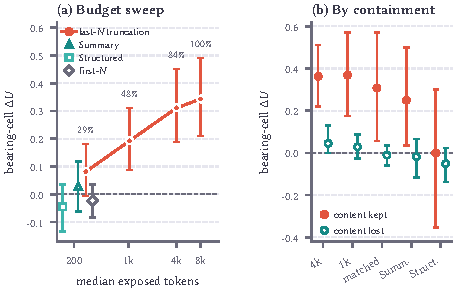
\includegraphics[width=\columnwidth]{fig_lenctl}
\caption{Length-control run on LongMemEval-V2: $\Delta U$ on the
$\lcBearCells$ bearing cells, task-clustered 95\% intervals.
\textbf{(a)}~Raw truncated to its last 4,096 and 1,024 tokens and to each
cell's Summary length (line), against Summary, Structured and the first-$N$
window at that length; percentages give the share of cells whose text still
contains the bearing content. \textbf{(b)}~The same arms split by whether
their text kept the bearing content (filled) or lost it (hollow).}
\label{fig:lenctl}
\Description{Left: bearing-cell utility rising with exposed tokens from about 0.08 at 280 tokens to 0.34 at 8,000, with Summary, Structured and first-N near zero. Right: for each arm, utility near 0.25 to 0.37 when the bearing content is kept and near zero when it is lost, except Structured whose kept estimate is near zero with a wide interval.}
\end{figure}

The length control was frozen before execution. Its extractive arm keeps the
final $N$ tokens of the same source segment, with $N$ set per cell to that
cell's own Summary token count, so it matches Summary's budget without any
model choosing content; a second arm keeps the first $N$ tokens instead, and
last-$N$ versus first-$N$ was registered as the decisive contrast. All three
pre-registered contrasts are computed on the $\lcBearCells$ bearing cells
(two replicate rows each, $\lcPrimaryN$ rows) and clustered over
$\lcBearTasks$ tasks: extractive versus Summary ($\lcPrimary$
$[\lcPrimaryLo, \lcPrimaryHi]$), Raw versus matched extractive ($\lcBudget$
$[\lcBudgetLo, \lcBudgetHi]$), and last-$N$ versus first-$N$ ($\lcEnds$
$[\lcEndsLo, \lcEndsHi]$).

The same run truncated Raw to its last 4,096, 1,024 and 20,000 tokens; the last
equals Raw, since no segment is longer. Table~\ref{tab:sweep} gives each arm's
bearing-cell $\Delta U$, its retention of the bearing content, and $\Delta U$
split by retention. \texttt{make\_lenctl.py} computes every entry from the row
file, whose checksum it verifies against the run manifest, and first checks
that it reproduces the three pre-registered contrasts. The run is not strictly
one session: $\lfLcCacheHits$ responses came from a cache filled minutes
earlier, and $\lcNullRows$ rows with a null reward are excluded, never zeroed.

\begin{table}[t]
\centering\footnotesize
\setlength{\tabcolsep}{2.4pt}
\caption{Length-control run on LongMemEval-V2: bearing-cell $\Delta U$ by arm
($\lcBearCells$ cells, task-clustered 95\% intervals), share of cells whose text
still contains the bearing content, and $\Delta U$ split by whether it does.
Exploratory beyond the three pre-registered contrasts.}
\label{tab:sweep}
\begin{tabular}{@{}lrrrrr@{}}
\toprule
arm & median tokens & kept & $\Delta U$ & $\Delta U\mid$kept & $\Delta U\mid$lost \\
\midrule
Raw (full) & \lcRawTok & \lcRawKept\% & \lcRawM\ [\lcRawLo, \lcRawHi] & \lcRawKM & -- \\
last 4,096 & \lcFourTok & \lcFourKept\% & \lcFourM\ [\lcFourLo, \lcFourHi] & \lcFourKM & \lcFourLM \\
last 1,024 & \lcOneTok & \lcOneKept\% & \lcOneM\ [\lcOneLo, \lcOneHi] & \lcOneKM & \lcOneLM \\
last $N$ (matched) & \lcMatchTok & \lcMatchKept\% & \lcMatchM\ [\lcMatchLo, \lcMatchHi] & \lcMatchKM & \lcMatchLM \\
Summary & \lcSumTok & \lcSumKept\% & \lcSumM\ [\lcSumLo, \lcSumHi] & \lcSumKM & \lcSumLM \\
Structured & \lcStrTok & \lcStrKept\% & \lcStrM\ [\lcStrLo, \lcStrHi] & \lcStrKM & \lcStrLM \\
first $N$ (matched) & \lcFirstTok & \lcFirstKept\% & \lcFirstM\ [\lcFirstLo, \lcFirstHi] & -- & \lcFirstLM \\
\bottomrule
\end{tabular}
\end{table}

\paragraph{Is the kept subset easier?} Retention is a property of the text,
fixed before any outcome, but the cells where a compressed text keeps the
content could still be easier ones. They are not for Summary or the matched
truncation: on the same cells, Raw gains $\lcSelSumKept$ where Summary kept the
content and $\lcSelSumLost$ where it lost it ($\lcSelMatchKept$ and
$\lcSelMatchLost$ for the matched truncation). For Structured the kept cells are
\emph{harder} ($\lcSelStrKept$ against $\lcSelStrLost$), which accounts for
its low kept estimate.

\paragraph{Position.} Target position is identical across all eight arms
within each cell (asserted). Between strata its distribution differs mildly
($\chi^2$ $p = \lcPosChiP$); the position-standardized Raw
\textsc{bearing}$-$control contrast is $\lcPosStd$ against $\lcPosUnadj$
unadjusted, and positive at every position.

\subsection{Formation-cost sensitivity}
\label{sec:reuse}
Formation cost per cell is the writer's tokens divided by the reuse factor
$r$, the number of cells that share one written memory. Our design fixes
$r = \frReuse$, so we recompute exposure efficiency over $r$ from the same
utilities and token counts (Figure~\ref{fig:reuse}). One Summary costs about
$\raFormSum$ writer tokens and one Structured record about $\raFormStr$. On
point estimates Summary overtakes Raw only for $r \gtrsim \raReuseStar$, but
its utility interval spans zero at every $r$, so the crossing point is not
estimated with any precision. Under the sparsity we measure, a memory that
bears on one task may be shown for few others, which pushes $r$ down and
formation cost up. The relevant factor in deployment is exposures per write,
not cells per memory. Input and output tokens are priced identically and prompt
caching is ignored; since output tokens usually cost more, both choices
understate the writer's cost.

\begin{figure}[t]
\centering
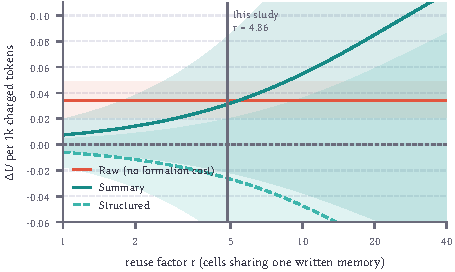
\includegraphics[width=\columnwidth]{fig_reuse}
\caption{Exposure efficiency ($\Delta U$ per thousand charged tokens) against
the reuse factor, on the $\frCells$ representation cells of LongMemEval-V2.
Lines use each representation's paired \textsc{bearing}$-$control effect;
bands use its 95\% interval over memories. Raw has no writer call and does not
depend on $r$. The vertical line marks the reuse factor of this study.}
\label{fig:reuse}
\Description{Line chart of efficiency against reuse factor on a log axis: Raw is flat near 0.034, Summary rises and crosses Raw near r of 5.5 with a wide band spanning zero, Structured is below zero.}
\end{figure}

\section{Second reader and writer, $\times$, reader factorial}
\label{sec:readerfull}

\paragraph{Design.}
The second-reader study was pre-registered before any design-cell call was
issued, with no transfer, the same ordering at a different magnitude, and a
different representation preference all committed as valid outcomes. The
memory file, prompt, filler pool, every rendered request, and each cell's
target position were hash-asserted against the first run at call time, and
the text re-verified byte-identical on $\rgRows$ rows; in the session-matched
run all $\smIdentK$ of $\smIdentN$ joinable rows are hash-identical.

\paragraph{Session-matched result.}
Both readers ran in one session. Over $\rgSmCells$ matched Raw cells on
$\rgSmTasks$ tasks ($\rgSmN$ replicate rows; these three counts are different
units), mean $\Delta U$ is $\rgSmOss$ under the first reader and $\rgSmGem$
under the second, a paired change of $\rgSmDiff$ $[\rgSmLo, \rgSmHi]$. The
two readers' own 95\% intervals overlap; plotting those would invite a ``no
difference'' reading that the paired design rules out. The within-memory
\textsc{bearing}$-$control contrast is $\rgBmcRawOss$ $[\rgBmcRawOssLo,
\rgBmcRawOssHi]$ under the first reader and $\rgBmcRawGem$ $[\rgBmcRawGemLo,
\rgBmcRawGemHi]$ under the second ($\rgBmcRawOssMem$ memories). The no-memory
arm moves by $\rgWithoutDelta$, so part of the gain is a weaker reader rather
than a better memory.

\paragraph{Cross-session first execution.}
A first execution with the two readers a day apart returned $\rgRawDiff$
$[\rgRawLo, \rgRawHi]$, inside the session-matched interval. Re-run together,
that difference splits into $-0.0327$ attributable to the session and
$-0.0364$ to the reader, which halves the apparent reader share. We quote only
the session-matched estimate.

\paragraph{Cell-level agreement, session-matched run.}
These are the numbers behind Figure~\ref{fig:overview}f. Over the
$\rgSmCells$ matched Raw cells, the readers' three-way labels (helped,
unchanged, hurt) agree on $\raReaderLabAgree$ of $\rgSmCells$ cells, at Cohen's
$\kappa = \raReaderKappa$; $\smCZeroZero$ cells are unchanged under both and
can only agree. Of the $\raReaderMoving$ cells that move under either reader,
both mark $\smAgree$ as helped, and signs agree on $\smAgree$ of the $\smBoth$
cells that move under both. The readers agree on no harmed cell (the first
reader's $\raHurtOss$ and the second's $\raHurtGem$ do not overlap), but so few cells
are harmed that this cannot show whether harm labels reproduce.

\paragraph{Cell-level agreement, earlier cross-session run.}
The first execution, with the two readers a day apart, covers a slightly
different matched set ($\rgRawN$ cells) and is the only source for Summary and
Structured. There the readers' per-cell $\Delta U$ correlate at
$r{=}\rgRawRAll$ over all cells, of which $\rgRawZeroBoth$ are zero under both;
over the $\rgRawNNz$ cells non-zero under either reader, $r = \rgRawRNz$
($\rgSumRNz$ for Summary, $\rgStrRNz$ for Structured). Signs agree on
$\rgRawSignK$ of $\rgRawSignN$ Raw cells where both move, and labels on
$\rgRawLabK$ of $\rgRawLabN$. Summary $\rgSumDiff$ $[\rgSumLo, \rgSumHi]$ and
Structured $\rgStrDiff$ $[\rgStrLo, \rgStrHi]$ span zero with only
$\rgSumNNz$ and $\rgStrNNz$ cells non-zero under either reader. Because this
run spans sessions, its numbers mix reader and session differences, and they
should not be pooled with the session-matched ones. Costs are not pooled
across readers: the second reports no reasoning-token counts.

\paragraph{Writer, $\times$, reader factorial.}
\label{sec:factorial}
All four writer--reader arms ran in one session. Every one of the eight
contrasts (writer, reader, same-family and interaction, on Summary with
$n{=}274$ and Structured with $n{=}268$) spans zero. The intervals are
informative rather than underpowered: they exclude writer and same-family
effects larger than $0.0380$, against the $\rgSmDiff$ reader effect the same
apparatus detects. Raw has no writer and is not in the factorial, and two
checkpoints form a $2\times2$ design, not a population of models.

\section{Cross-benchmark contrasts}
\label{sec:crossbenchtable}
The one quantity all three benchmarks define identically is the per-cell
representation contrast: a representation's $\Delta U$ minus Raw's on the same
memory and task. It separates from zero on LongMemEval-V2 alone
(Figure~\ref{fig:overview}e): Summary$-$Raw is $\xbSRLmM$
$[\xbSRLmLo, \xbSRLmHi]$ and Structured$-$Raw is $\xbTRLmM$
$[\xbTRLmLo, \xbTRLmHi]$ on $\xbSRLmN$ cells. On SciCode ($n{=}\xbSRScN$) and
SWE-bench Verified ($n{=}\xbSRSwN$) every interval includes zero, but there the
memories themselves have no effect even in raw form: Raw's own $\Delta U$ is
$\rvSciRaw$ $[\rvSciRawLo, \rvSciRawHi]$ on SciCode, where $\rvSciRawTied$ of
$\rvSciRawN$ cells are unchanged, and $\rvSweRaw$ $[\rvSweRawLo, \rvSweRawHi]$
on SWE-bench. With no Raw effect to preserve or lose, a representation contrast
there is uninformative about representation; these benchmarks bound where
memory matters for this reader, not how it should be written
(Section~\ref{sec:crossbenchtable}).

Table~\ref{tab:crossbench} gives the values plotted in
Figure~\ref{fig:overview}e. We compare contrasts rather than
per-representation $\Delta U$ because each benchmark carries its own
nondeterminism. The no-memory arm, whose input is identical across
representations, still disagrees with itself on
$\xbFloorLmK/\xbFloorLmN{=}\xbFloorLm$ of LongMemEval-V2 cells and
$\xbFloorScK/\xbFloorScN{=}\xbFloorSc$ of SciCode cells, and a paired contrast
removes that term. SWE-bench has no such floor because its no-memory arm is
deterministic by construction. SciCode's equivalent judge control disagrees
on 5 of 135 cells within one session, so determinism cannot be assumed of a
new benchmark.

\begin{table}[t]
\centering\footnotesize
\setlength{\tabcolsep}{4pt}
\caption{Per-cell representation contrasts: $\Delta U$ under one
representation minus $\Delta U$ under Raw on the same memory and task, with
task-clustered 95\% intervals. Only LongMemEval-V2 separates from zero. Every
SciCode and SWE-bench interval includes zero (SWE-bench's Summary$-$Raw only at
its upper bound), and doubling the SciCode cell
count separated no contrast. MDE is the minimum detectable contrast at 80\%
power and two-sided $\alpha = 0.05$, computed from each interval's width.
Raw's own with-versus-without $\Delta U$ is $\rvSciRaw$
$[\rvSciRawLo, \rvSciRawHi]$ on SciCode and $\rvSweRaw$ on SWE-bench, so on
these benchmarks no memory effect exists for a representation to preserve, and
the contrasts cannot test the ordering.}
\label{tab:crossbench}
\setlength{\tabcolsep}{3pt}
\begin{tabular}{@{}llrrrr@{}}
\toprule
contrast & benchmark & $n$ & mean & 95\% CI & MDE \\
\midrule
Summary$-$Raw
 & LongMemEval-V2 & \xbSRLmN & \xbSRLmM & [\xbSRLmLo, \xbSRLmHi] & \raMdeSRLm \\
 & SciCode        & \xbSRScN & \xbSRScM & [\xbSRScLo, \xbSRScHi] & \raMdeSRSc \\
 & SWE-bench      & \xbSRSwN & \xbSRSwM & [\xbSRSwLo, \xbSRSwHi] & \raMdeSRSw \\
\midrule
Structured$-$Raw
 & LongMemEval-V2 & \xbTRLmN & \xbTRLmM & [\xbTRLmLo, \xbTRLmHi] & \raMdeTRLm \\
 & SciCode        & \xbTRScN & \xbTRScM & [\xbTRScLo, \xbTRScHi] & \raMdeTRSc \\
 & SWE-bench      & \xbTRSwN & \xbTRSwM & [\xbTRSwLo, \xbTRSwHi] & \raMdeTRSw \\
\bottomrule
\end{tabular}
\end{table}

\section{Sign reversal and the decomposition}
\label{sec:negative}
\paragraph{Why flip rates cannot be compared across strata.}
A memory can show a flip only if at least two of its cells move with opposite
signs, so the chance of a flip grows with the number of cells per memory. In
the screened design a memory has $\raCellsPerMemBear$ \textsc{bearing} cells
and $\raCellsPerMemRand$ \textsc{random} cells on average. The naive
contrast (0 of 35 \textsc{bearing} memories against 17 of 60 \textsc{random},
Fisher one-sided $p = 1.5\times10^{-4}$) therefore mostly reflects that
difference. To test this, we took each of the $\raMatchedN$ memories with at
least two \textsc{bearing} cells and drew, without replacement, as many of its
\textsc{random} cells as it has \textsc{bearing} cells, then recounted flips
(20{,}000 resamples). The random stratum averages $\raMatchedMean$ flips and
shows none in $\raMatchedPZero\%$ of resamples (Figure~\ref{fig:reversal}b), so
0 of 35 is what chance alone would most often produce. A Wilson bound on the \textsc{bearing} flip rate would also treat 35 memories
from 21 episodes as independent.
Matching each memory's random subsample on the no-memory outcome as well (so
both strata get the same opportunities to help and to hurt) leaves all
$\lfCondFlipMems$ memories eligible; the random stratum then shows a mean of
$\lfCondFlipMean$ flips and none in $\lfCondFlipPZero\%$ of resamples. We
therefore do not compare flip rates across strata.

\paragraph{Why the sign of moving cells is not a comparison either.}
A tempting alternative compares the share of negative cells among cells that
move: $\raNegBearK$ of $\raNegBearN$ for \textsc{bearing} against
$\raNegRandK$ of $\raNegRandN$ for \textsc{random}. That comparison is
confounded by baseline accuracy. A memory can only hurt where the reader was
correct without it, and \textsc{bearing} tasks have the lowest no-memory
accuracy, so they offer the fewest chances to hurt.

\paragraph{Transitions conditioned on the no-memory outcome.}
Reward is binary in the screened run: each stratum's mean equals
(helped $-$ hurt)$/n$ exactly. With Table~\ref*{M-tab:screened}'s both-arms-fail
rate this fixes the full transition table (Table~\ref{tab:transitions}).
Conditioned on opportunity, the strata do not differ detectably in harm,
and they differ sharply in help (Figure~\ref{fig:reversal}a). In the
\textsc{random} stratum help and harm rates are close, the signature of a
content-independent response to inserting an item, which we treat as the
perturbation floor (\main{sec:metrics}). The table's Wilson intervals treat cells as
independent. Resampling memories instead, the harm rates have intervals of
$[\lfHurtClBearLo, \lfHurtClBearHi]$ (\textsc{bearing}),
$[\lfHurtClCtrlLo, \lfHurtClCtrlHi]$ (control) and
$[\lfHurtClRandLo, \lfHurtClRandHi]$ (\textsc{random}), which overlap, and the
help rates $[\lfHelpClBearLo, \lfHelpClBearHi]$,
$[\lfHelpClCtrlLo, \lfHelpClCtrlHi]$ and $[\lfHelpClRandLo, \lfHelpClRandHi]$,
where \textsc{bearing}'s is disjoint from the others. Both
analyses here are exploratory and are produced by
\texttt{make\_reanalysis.py}, which first checks that it reproduces every flip
count and stratum mean in the paper.

\begin{table}[t]
\centering\footnotesize
\setlength{\tabcolsep}{2.6pt}
\caption{Screened run on LongMemEval-V2: transitions between the no-memory
and with-memory outcome (binary reward). Accuracy columns give the share of
cells answered correctly without and with the memory. Hurt is conditioned on
cells correct without the memory, help on cells wrong without it; Wilson 95\%
intervals in brackets.}
\label{tab:transitions}
\begin{tabular}{@{}lrrrrr@{}}
\toprule
stratum & $n$ & acc.\ w/o & acc.\ with & hurt $\mid$ correct & help $\mid$ wrong \\
\midrule
\textsc{bearing} & \spBearN & \raAccZeroBear & \raAccOneBear
  & \raHurtRateBear\ [\raHurtLoBear, \raHurtHiBear] & \raHelpRateBear\ [\raHelpLoBear, \raHelpHiBear] \\
control & \spCtrlN & \raAccZeroCtrl & \raAccOneCtrl
  & \raHurtRateCtrl\ [\raHurtLoCtrl, \raHurtHiCtrl] & \raHelpRateCtrl\ [\raHelpLoCtrl, \raHelpHiCtrl] \\
\textsc{random} & \spRandN & \raAccZeroRand & \raAccOneRand
  & \raHurtRateRand\ [\raHurtLoRand, \raHurtHiRand] & \raHelpRateRand\ [\raHelpLoRand, \raHelpHiRand] \\
\midrule
\multicolumn{6}{@{}l}{\emph{opportunities:} hurt $\raHurtOppBear$ / $\raHurtOppCtrl$ / $\raHurtOppRand$ cells;
help $\raHelpOppBear$ / $\raHelpOppCtrl$ / $\raHelpOppRand$ cells} \\
\bottomrule
\end{tabular}
\end{table}

\paragraph{The additive-null comparison.}
Fitting $\mu + a_m + b_t$ and simulating from it, the excess of the observed
reversal rate over the fitted additive model is negative in all three strata.
Two independent implementations agree on the sign and disagree on the
magnitude, so we quote only the sign.

\paragraph{Why the decomposition is not identifiable.}
The within-session execution floor is exactly zero: replicates issued 0--16
seconds apart agree on 1{,}157 of 1{,}157 cells. With no residual scale, the
fitted residual collapses and the task and interaction shares are not
separately identified, so we report none. Clean per-cell utilities and a
variance decomposition are in tension on a reader without execution noise.

\begin{figure}[t]
\centering
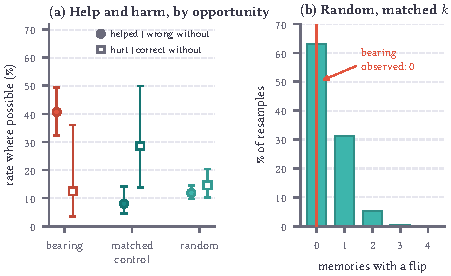
\includegraphics[width=\columnwidth]{fig_reversal}
\caption{Sign reversal on LongMemEval-V2, screened design (1{,}157 cells,
60 memories). \textbf{(a)}~Help rate among cells the reader got wrong without
the memory (filled) and harm rate among cells it got right (hollow), with
Wilson 95\% intervals; counts are in Table~\ref{tab:transitions}. Harm does not differ detectably across
strata; help does. \textbf{(b)}~Flips among the 35 memories with at least two
\textsc{bearing} cells when each memory's \textsc{random} cells are subsampled
to its own \textsc{bearing}-cell count (20{,}000 resamples); the line marks the
observed \textsc{bearing} count.}
\label{fig:reversal}
\Description{Left: dot plot of help and harm rates by stratum; help is about 41 percent for bearing against 8 and 12 percent elsewhere, harm overlaps across strata at 12 to 29 percent with wide intervals. Right: histogram of flip counts at matched cell counts, with zero flips in about 63 percent of resamples.}
\end{figure}

\section{Data, code and prompt availability}
\label{sec:repro}
\label{sec:prompts}
\paragraph{Public dataset.} The Conditional Memory Utility Dataset is available on
\href{https://huggingface.co/datasets/AgentsSci/AAMAS2027-ConditionalMemory}{Hugging Face}.
The frozen \texttt{v0.6-}\allowbreak\texttt{length-control} snapshot contains 16,816 records:
16,535 from LongMemEval-V2, 154 from SciCode, and 127 from SWE-bench Verified.
A row describes a memory--task pair under a representation, reader, condition
and replicate, with the outcome under each arm, available output text and
cost metadata. Missing or unscorable measurements remain explicitly marked;
they must not be converted to zero rewards.

\paragraph{Version and reproducibility.} The data file is
\texttt{data/}\allowbreak\texttt{cells.jsonl}. The repository also provides a manifest with file checksums, schema and validation
code, and documentation of the included conditions and upstream sources.
Readers can download the data directly or pin the
\texttt{v0.6-}\allowbreak\texttt{length-control} revision with the Hugging Face client. The data
card contains a runnable download example and explains the validation warnings.
This snapshot was built on 2 October 2026 and does not contain every later
manuscript analysis; in particular, its condition inventory does not include
the fixed-total-context experiment. The public Hub package contains schema and
validation code, not the complete experiment, analysis and prompt bundle.
The length-control identity arm is an A/A control and must not be pooled with
Raw as an independent condition. Per-pair utility labels describe the recorded
evaluation conditions, rather than unconditional training targets.

\paragraph{Withheld and missing text.} The 154 SciCode records contain Raw
memories; their reader outputs were not retained. SciCode Summary and Structured
records are absent because their memory text was not persisted. The 127
SWE-bench records provide identifiers and derived measurements, with restricted
corpus and output text withheld under the release policy. These are distinct
from records missing because of a persistence gap. The data card documents the
sentinels and per-source reuse terms; access to the dataset does not grant a
new license to withheld upstream content.

\section{Extended limitations}
\label{sec:extlimits}

\paragraph{Leakage rates are lower bounds.}
Our leakage detector reuses the benchmark's phrase matcher, whose normalizer
strips punctuation without inserting a space. A gold phrase next to a quote
or an equals sign is glued to its neighbor and the match fails. Such leaks
are missed, and punctuation is common in accessibility trees, so every
leakage rate we report is a lower bound. A control test records the defect, so
an upstream fix would be detected. The 156
LLM-judged questions cannot be audited without an inference call and are
recorded as undecidable rather than clean. 69 multiple-choice questions with
gold answers of one to five characters cannot be audited structurally and are
never folded into a pooled rate.

\paragraph{The judge floor measures decoding.}
$F_{\mathrm{judge}}$ is zero wherever we measured it: over $\lfJudgeObs$
explicit re-scorings of $\lfJudgeUnits$ units in the earlier official arm, and
in every stratum of the screened run. Both estimators carry a positive control
(a planted disagreement makes them fire). A zero floor here reflects a
deterministic scorer and greedy decoding, not an unambiguous rubric. The
SciCode control in Section~\ref{sec:crossbenchtable}, which disagrees on 5 of
135 cells, is a different scorer on a different benchmark. We have no
cross-session floor for any arm and presume it to be non-zero.
%%% NOTE: earlier drafts quoted "240 of 240" and "288 re-scorings"; neither
%%% figure could be traced to a ledger in results/, so both were replaced.

\paragraph{Semantic type.}
We intended semantic memory type as a second axis, but in our representation
pilot the two labeling passes agreed on 3 of 8 segments at Cohen's
$\kappa = 0.000$: the structured writer's own pass called every segment
\texttt{episodic}, a degenerate marginal, so we report no semantic-type
breakdown. Separately, exactly one deterministically scorable
\emph{errors-gotchas} question exists in the benchmark and accounts for 865 of
6{,}920 web cells, so any per-stratum result there is a single-question result.

\paragraph{Writer failures and faithfulness.}
The structured writer failed on 3 of 60 segments, all by exhausting the token
budget mid-value rather than by malformed output, and on 0 of the 57 writes
that finished. An 8-segment pilot had put the failure rate at 0 of 8 and could
not have seen this, since it never reached the cap. Our faithfulness measures
are a screen, not a guarantee: a low score is strong evidence of a problem,
a high score is weak evidence of its absence, and they do not detect
recombination, omission, unsupported inference or negation.

\paragraph{Unrecorded quantities.}
Two quantities were not recorded during the runs and cannot be recovered: how
many gold-free picks contain the answer, and how the 12 position-probe cells
were chosen, which is why we treat that probe as a pilot.

\paragraph{Stated exclusions.}
17 of the 295 deterministically scored questions have no memory unit that
carries their gold answer under the segmentation answerability check, so their
cells can only yield $\Delta U \le 0$. The bearing screen, a looser containment
test, fires on no unit for $\soScrZero$ of them (Section~\ref{sec:sophia}).
23 of the 1{,}889 units (1.2\%) are their entire trajectory.

\section{Pre-registration record}
\label{sec:prereg}
Each pre-registered analysis was fixed in a pre-commitment document in the code
repository before the data it governs existed. The documents are released with
the code. To preserve anonymity we omit their commit identifiers here; the
release links each one to a commit and its timestamp, so its timing can be
checked on de-anonymization. Table~\ref{tab:prereg} lists every pre-registered analysis, its
anchor, and every deviation the run ledgers record. Pre-commitments were not edited after
the fact; where a result does not match one, the mismatch is reported.

\begin{table}[h]
\centering\footnotesize
\setlength{\tabcolsep}{3pt}
\caption{Pre-registered analyses, their anchors, and recorded deviations.}
\label{tab:prereg}
\begin{tabular}{@{}p{0.27\columnwidth}p{0.30\columnwidth}p{0.37\columnwidth}@{}}
\toprule
analysis & anchor & recorded deviation \\
\midrule
screened design and its reduction criterion & criterion fixed in code before the numbers existed & none recorded \\
reversal rate (headline) & pre-registration, section~5 & comparison with an additive null added later, as a diagnostic \\
variance decomposition & pre-registration, section~6 & not identifiable here (zero execution floor); in earlier arms the mixed model did not converge and the registered fallback was used \\
gold-free screens & gold-free screen pre-commitment & none recorded \\
length control & frozen at a recorded commit, before execution & \lfPrLcMismatch\ of \lfPrLcCompared\ descriptive figures do not re-derive: bearing quartile means by Raw length; none appears in the paper \\
second reader & written before any design-cell call & cross-session estimate superseded by a session-matched run \\
session-matched reader run & falsifiers committed before data & none recorded \\
writer\,$\times$\,reader factorial & factorial pre-commitment & one prose sign error ($-\tfrac12$ for $+\tfrac12$ interaction); replication check fails on sign only \\
SciCode scale-up & scale-up pre-commitment & none recorded \\
\bottomrule
\end{tabular}
\end{table}

\paragraph{The two deviations that bear on results.} The additive-null
comparison of reversal rates (\main{sec:r0}) was \emph{not} pre-registered;
the registered headline is the reversal rate itself, and the comparison is a
diagnostic added afterwards. In the writer\,$\times$\,reader factorial, the
registered criterion asked the re-measured reader effect to reproduce the
earlier one in sign and significance. Both estimates are near zero and span
zero (Summary $\lfPrWfSumOld$ then $\lfPrWfSumNew$, Structured
$\lfPrWfStrOld$ then $\lfPrWfStrNew$), so the significance verdict reproduces
and the sign does not; the two intervals contain each other's point estimates.
The factorial's pre-commitment also states that the same-family effect equals
$-\tfrac12$ of the interaction; the correct relation, which the analysis code
checks numerically, is $+\tfrac12$. Every quantity was computed as registered.

\section{Follow-up runs}
\label{sec:sophia}
Three follow-up runs test the main results under conditions the main design
held fixed; all are exploratory and used the same serving endpoint and reader as
the main runs. A generator script in the released code computes every number
below from the row files.

\paragraph{Second session, randomized position.} All $\soXoneCells$ bearing and
control cells, three replicates each, the memory's position redrawn per
replicate ($\soXoneCalls$ real calls, $\soXoneCacheHits$ from cache,
$\soXoneErr$ failed and excluded). Bearing minus control, paired within memory:
$\soXoneD$ $[\soXoneLo, \soXoneHi]$ over $\soXoneMems$ memories;
episode-clustered $[\soXoneEpLo, \soXoneEpHi]$ ($\soXoneEps$ episodes); two-way
(memory $\times$ task) $\soXoneTw$ $[\soXoneTwLo, \soXoneTwHi]$. Across the
three positions of a cell, the label changes in $\soPosChg$ of $\soPosCells$
cells ($\soPosChgPct\%$), and in $\soPosChgMv$ of the $\soPosMov$ cells that move
at least once ($\soPosChgMvPct\%$); position accounts for $\soPosVarPct\%$ of
the variance of $\Delta U$. Joined one-to-one to the published run, labels agree
in $\soStabSamePct\%$ of $\soStabSameN$ replicate-cells at the same position
($\kappa = \soStabSameK$) and in $\soStabDiffPct\%$ of $\soStabDiffN$ at a new
one ($\kappa = \soStabDiffK$).

\paragraph{Fixed total context.} $\soXtwoCells$ cells over $\soXtwoMems$
memories, two replicates. For each cell, $T$ is the base filler plus the Raw
memory; every other arm, and the no-memory arm, is padded after the base context
with bearing-disjoint filler to $T$ (asserted equal across arms), the memory
kept at its K2 position. \emph{Disclosed defect:} the no-memory cache key was
(trajectory, task, replicate), so two memories from one trajectory paired with
one task could share a no-memory response although their padding differs. The
headline numbers exclude all $\soXtwoCollCells$ such cells ($n=\soFN$ bearing
cells); including them ($n=\soFNAll$) changes no conclusion:

\begin{table}[!ht]
\centering\footnotesize
\setlength{\tabcolsep}{3pt}
\caption{Bearing-cell $\Delta U$ at a fixed total context (task-clustered
95\% intervals).}
\label{tab:fixedctx}
\begin{tabular}{@{}lll@{}}
\toprule
arm & excluding exposed cells & all cells \\
\midrule
Raw & \soFRaw\ [\soFRawLo, \soFRawHi] & \soFRawAll\ [\soFRawAllLo, \soFRawAllHi] \\
Summary & \soFSum\ [\soFSumLo, \soFSumHi] & \soFSumAll\ [\soFSumAllLo, \soFSumAllHi] \\
Structured & \soFStr\ [\soFStrLo, \soFStrHi] & \soFStrAll\ [\soFStrAllLo, \soFStrAllHi] \\
matched truncation & \soFTr\ [\soFTrLo, \soFTrHi] & \soFTrAll\ [\soFTrAllLo, \soFTrAllHi] \\
Summary $-$ Raw & \soFSumR\ [\soFSumRLo, \soFSumRHi] & \soFSumRAll\ [\soFSumRAllLo, \soFSumRAllHi] \\
Structured $-$ Raw & \soFStrR\ [\soFStrRLo, \soFStrRHi] & \soFStrRAll\ [\soFStrRAllLo, \soFStrRAllHi] \\
\bottomrule
\end{tabular}
\end{table}

The matched truncation is sensitive to the exclusion and supports no claim. The
cache key now includes the memory, so a re-run cannot repeat the defect.

\paragraph{Retrieval.} The reference labels are the screened design's (75 tasks, 266
bearing edges, reproduced and asserted). Each method ranks the task's whole
domain pool by the raw question; dense retrieval embeds 512-token chunks (a
unit scores its best chunk) or the first 2{,}000 tokens.

\begin{table}[!ht]
\centering\footnotesize
\setlength{\tabcolsep}{3pt}
\caption{Retrieval of bearing units (task-clustered 95\% intervals; chance
recall@10 is about \soChanceTenP). MRR is the mean reciprocal rank of the first
bearing unit; AUROC is the area under the ROC curve over bearing and
non-bearing units.}
\label{tab:retrieval}
\begin{tabular}{@{}lllll@{}}
\toprule
method & recall@1 & recall@10 & MRR & AUROC \\
\midrule
BM25 & \soRBmOne & \soRBmTen\ [\soRBmTenLo, \soRBmTenHi] & \soRBmMrr & \soRBmAuc \\
dense, prefix & \soRPreOne & \soRPreTen\ [\soRPreTenLo, \soRPreTenHi] & \soRPreMrr & \soRPreAuc \\
dense, chunks & \soRChkOne & \soRChkTen\ [\soRChkTenLo, \soRChkTenHi] & \soRChkMrr & \soRChkAuc \\
\bottomrule
\end{tabular}
\end{table}

Of the 295 deterministic questions, $\soScrZero$ fire on no unit, $\soScrDisc$
on one to eight, and $\soScrOver$ on more than eight. Without the cap, string
containment fires for all $\soNoCapMems$ memories, on $\soNoCapMin$ to
$\soNoCapMax$ tasks each.

\paragraph{Variance decomposition.} In the second-session run each cell has three
replicates at redrawn positions, which supplies the residual scale the main run
lacked. On the $\rvDecCells$ cells with all three replicates we fit the additive
model $\mu + a_m + b_t$ to cell means by least squares; its residual mean square
($\rvDecDf$ degrees of freedom) estimates the interaction variance plus the
within-cell variance divided by three, and the within-cell variance estimates the
residual. The shares are $\rvIntShare\%$ interaction, $\rvAddShare\%$ additive
memory and task effects, and $\rvEpsShare\%$ position with decoding; the
interaction $F$ test gives $F=\rvIntF$ ($p\rvIntP$). This is a method-of-moments
estimate on a sparse crossed design, reported as exploratory.

\paragraph{Power for harm.} With $16$ bearing cells able to show harm, against
the random stratum's rate of $\rvHarmRandPct\%$, the screened design detects
(80\% power, two-sided $\alpha=0.05$) only a bearing harm rate of
$\rvHarmMdePct\%$ or more; the null on harm is therefore weak evidence.

\paragraph{Containment inside the random-task stratum.} Memories in this stratum are real
same-domain pages. On the $\rvRandFireN$ random cells where the containment
detector fires (at any breadth) the memory helps in $\rvRandFireHelp\%$ of the
$\rvRandFireHelpN$ cells the reader got wrong without it, against
$\rvRandSilentHelp\%$ of $\rvRandSilentHelpN$ where it is silent; harm is
$\rvRandFireHurt\%$ and $\rvRandSilentHurt\%$. Part of the random stratum's help
is content, so its help rate bounds pure perturbation from above.

\paragraph{The gold-free screen over the full universe.} The model-based screen
was applied to all $\rvGfUniverse$ (task, unit) pairs: an exhaustive lexical
stage kept $\rvGfCand$ candidates, and the judge confirmed $\rvGfYes$ over
$\rvGfTasks$ tasks and $\rvGfMems$ memories, under the same cap of eight units
per task. A gold-free definition does not make bearing denser.

\paragraph{Sparsity across screen caps.} Recomputing the screen over the
deterministic tasks at four caps on the number of units a task may fire on:
at a cap of 4, $\rvCapFourTasks$ tasks and $\rvCapFourMems$ bearing memories;
at 8 (the paper's screen), $\rvCapEightTasks$ and $\rvCapEightMems$; at 16,
$\rvCapSixteenTasks$ and $\rvCapSixteenMems$; at 32, $\rvCapThirtyTwoTasks$ and
$\rvCapThirtyTwoMems$. At every cap the median bearing memory bears on exactly one
task, and $\rvCapShareLo$--$\rvCapShareHi\%$ bear on exactly one. Only removing the
cap entirely makes containment fire for every memory.

\paragraph{Which memories were sampled.} The 60 memories are every memory that
bears on two or more tasks and passes the size cap ($\rvSelMulti$ of the
corpus's $\rvPopMulti$) plus $\rvSelSingle$ single-task memories. The headline
contrast is $\rvHeadSingle$ $[\rvHeadSingleLo, \rvHeadSingleHi]$ on the
single-task memories and $\rvHeadMulti$ $[\rvHeadMultiLo, \rvHeadMultiHi]$ on the
multi-task ones; reweighted to the $\rvPopAll$ bearing memories of the corpus, of
which $\rvPopSinglePct\%$ bear on one task, it is $\rvHeadW$
$[\rvHeadWLo, \rvHeadWHi]$ (memory bootstrap within each group).


\section{Additional figures}
\label{sec:figs}
Figure~\ref{fig:overview} collects views referenced from the main paper: bearing
breadth, helped cells by stratum, retrieval, the representation contrasts with
their token costs, the cross-benchmark contrasts, and the two readers'
agreement. Figure~\ref{fig:lenctl} (Section~\ref{sec:lengthcontrol}) details the
length-control run.



\begin{figure*}[p]
\centering
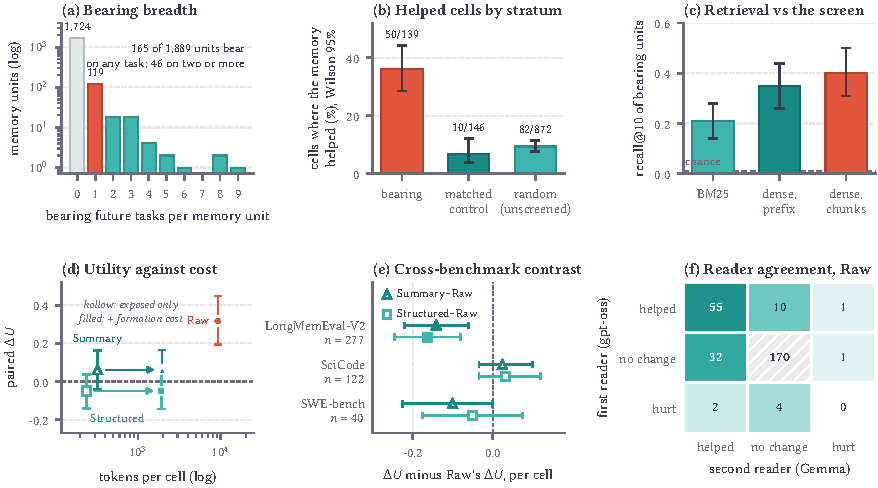
\includegraphics[width=\textwidth]{fig_results}
\caption{Overview of further results on LongMemEval-V2 (a--d, f) and across
benchmarks (e). \textbf{(a)}~Future tasks each of the $\bearUnits$ memory units
bears on, over $\bearDetTasks$ discriminative tasks (log axis).
\textbf{(b)}~Share of cells where the memory helped, cell-level Wilson 95\%
intervals (memory-resampled ones in Section~\ref{sec:negative}), for
the same $\spMems$ memories in three strata. \textbf{(c)}~Share of bearing units a retriever ranks in its top ten of the
domain pool (75 tasks, task-clustered 95\% intervals); the dashed line is
chance. \textbf{(d)}~Paired
\textsc{bearing}$-$control effect per representation ($\frCells$ cells,
$\frMems$ memories, intervals over memories); hollow markers count exposed
tokens, filled ones add formation cost amortized over $\frReuse$ cells.
\textbf{(e)}~Per-cell $\Delta U$ minus Raw's, task-clustered intervals; filled
markers exclude zero. \textbf{(f)}~Two readers' labels on $\rgSmCells$ Raw cells
in one session; the hatched cell (zero under both) cannot disagree.}
\label{fig:overview}
\Description{Six panels: a log histogram of bearing tasks per memory unit peaking at one; bar chart of helped-cell rates by stratum with bearing highest; similarity sextile lines nearly flat; utility against tokens showing Raw above zero and compressed representations near zero; cross-benchmark contrast intervals, only LongMemEval-V2 excluding zero; a three by three reader agreement table.}
\end{figure*}




%%%%%%%%%%%%%%%%%%%%%%%%%%%%%%%%%%%%%%%%%%%%%%%%%%%%%%%%%%%%%%%%%%%%%%%%

\clearpage
\section*{Supplementary Material}
\label{sec:supplementary-material}

% Use S1, S2, ... section numbering and S1, S2, ... figure/table numbering.
% Page numbering continues from the main paper.
\setcounter{section}{0}
\setcounter{subsection}{0}
\setcounter{figure}{0}
\setcounter{table}{0}
\renewcommand{\thesection}{S\arabic{section}}
\renewcommand{\thesubsection}{\thesection.\arabic{subsection}}
\renewcommand{\thefigure}{S\arabic{figure}}
\renewcommand{\thetable}{S\arabic{table}}

% References from the supplement to sections, tables, and figures in main.tex.
\providecommand{\main}[1]{main paper, Section~\ref*{M-#1}}

% Supplementary sections.
\noindent\textbf{Guide to this supplement.}
The paper is self-contained, and this document holds the detail behind it. Section~\ref{sec:protocol} gives the full protocol: how the
writer is kept blind to future tasks, how target position is controlled,
both gold-free screens, and the leakage audit.
Section~\ref{sec:benchdetails} describes the benchmark adapters, the scorer,
pairing and power, and why each secondary benchmark has the yield it has.
Section~\ref{sec:config} lists the frozen execution configuration, the noise
floors, the label definitions, and why the additive null and the variance
decomposition matter. Section~\ref{sec:lmresults} adds LongMemEval-V2
results: the cell-level sparsity map, the reader capability check, the
length-control design, and the formation-cost sensitivity. Section~\ref{sec:readerfull} reports the
second-reader study and the writer-by-reader factorial in full, and
Section~\ref{sec:crossbenchtable} gives the cross-benchmark contrasts as a
table. Section~\ref{sec:negative} reports the sign-reversal analysis the study
was designed around, including why naive sign comparisons mislead and the
transition analysis that replaces them. Section~\ref{sec:repro} covers data, code and
prompt availability, licensing and reproducibility, and
Section~\ref{sec:extlimits} the limitations not needed to read the main result. Section~\ref{sec:prereg} is the pre-registration record: every
pre-registered analysis, its anchor, and every recorded deviation. Section~\ref{sec:sophia} reports three follow-up runs: a second session
with randomized position, a fixed total context, and a retrieval evaluation. Every table and figure states its
benchmark, population and denominator.

\section{Protocol details}
\label{sec:protocol}

\subsection{Keeping the writer blind to future tasks}
\label{sec:taskblind}
Memory formation must be a function of the past episode alone, $m = W(e)$.
If the writer could see a future task, a positive $\Delta U$ would show only
that a model can be told the answer and copy it forward. We enforce this with
four structural barriers rather than by convention. (1)~\emph{Arity}: the
writer function takes a segment and nothing else. (2)~\emph{A closed field
set}: the writer emits only the fields of its schema. (3)~\emph{A metadata
denylist}: the weakest barrier, present to make a plumbing mistake fail loudly.
(4)~\emph{A single interpolation point}: the prompt has one placeholder, the
segment text. Each barrier carries a negative control that plants the defect
and requires the check to fire. Prompt identity is derived from the prompt
file's bytes, not from a hand-maintained version constant that could report a
stale version.

\subsection{Target position is held fixed}
\label{sec:position}
The \textsc{with} arm holds one more item than the \textsc{without} arm, so
some rule must place it, and that rule is not neutral. Holding the memory,
question, filler, model, decoding and seed fixed and varying only the
position of the target memory changes the answer in 8 of 12 probe cells. Measured at scale in the second-session
run (Section~\ref{sec:sophia}), position changes $\soPosChgPct\%$ of labels. A
comparison that does not control position therefore measures position
together with presence. We hold position fixed across replicates, vary it
across cells, and record it on every row. This is also what makes the
second-reader comparison (\main{sec:readertransfer}) a comparison of readers
and not of positions. The probe is small ($n{=}12$), and we treat the rate
as provisional.

\subsection{The bearing screen and both gold-free screens}
\label{sec:goldfree}
The bearing screen reads the memory text, the task's gold answer, and the
task's evaluation specification; it never reads the question. A pair is
\textsc{bearing} only when the benchmark's scorer marks the memory text
correct against the gold answer \emph{and} the test fires on at most eight of
the 865--1{,}024 units in the task's domain pool. The second clause matters.
An earlier, non-discriminative version of the flag fired on nearly every
candidate: its rate on paired versus unpaired memories was in a ratio of
$0.995$, so it said nothing about any one of them.

We pre-registered two gold-free screens before execution. Each reads the
memory, the question and the same-domain pool, and none of the gold answer,
the reward, any model output, or the evaluation specification. We report
both, because reporting only the screen that worked would select an
instrument on its outcome.
\begin{itemize}
\item \emph{Model-based screen.} The judge is $\lfGfJudge$, the reader's own
model, at temperature 0, asked whether the memory contains the specific
information the question asks about. On cells the gold screen never
selected, its picks move the reader from $\gfWithoutPct\%$ correct without the
memory to $\gfWithPct\%$ with it ($\gfN$ rows, $\gfCells$ cells); its matched
control moves from $\gfCtlWithoutPct\%$ to $\gfCtlWithPct\%$ ($\gfCtlN$ rows,
$\lfGfCtlCells$ cells). The contrast of $\gfDiff$ has a task-clustered interval
of $[\lfGfTaskLo, \lfGfTaskHi]$ ($\lfGfTaskN$ tasks), an episode-clustered one
of $[\lfGfEpLo, \lfGfEpHi]$ ($\lfGfEpN$ episodes), and a paired-by-memory
difference of $\lfGfMemD$ over $\lfGfMemN$ memories. Against the gold screen it
recovers $\lfGfBoth$ of $\lfGfGold$ gold-bearing pairs ($\lfGfRec\%$ recall),
and $\lfGfBoth$ of its $\lfGfPicks$ picks are gold-bearing ($\lfGfPrec\%$). The
run is in one session, separate from the gold run.
\item \emph{Lexical screen.} It returns no effect. A diagnostic independent of
any utility explains why: its bearing cells fail in both arms at a rate of
$\gfLexBaf$, \emph{worse} than unscreened random pairing, against
$\gfLlmBaf$ for the model-based screen. A criterion whose selections are
harder than a random draw has not located bearing pairs.
\end{itemize}

\subsection{Leakage audit}
\label{sec:leakage}
The writer invariant excludes \emph{task-directed writing}, not a naturally
occurring memory that happens to contain a later answer. Such a memory is
genuinely useful, and removing it would condition the cell set on the
outcome. We therefore audit every cell rather than filter it. The detector
reuses the benchmark's own scorer and asks whether the rendered memory text
alone would score correct against the gold answer. For \textsc{bearing} cells
the answer is yes by construction, since that is half the bearing definition.
The audit carries information for the control and \textsc{random} strata and
for the Summary and Structured texts, where containment is not guaranteed and
can be conditioned on in analysis. It is validated by 17
controls (plants it must catch, clean cases it must not fire on, and two
pinned known false negatives) and aborts if any control fails.

\subsection{Three kinds of zero in the cost ledger}
\label{sec:zeros}
Raw makes zero writer calls; Summary and Structured make one each per
segment. The ledger distinguishes three zeros that are routinely merged: a
measured zero (Raw makes zero extraction calls), an absent measurement (no
call was made, so the cell leaves that denominator), and an unreported field
(the endpoint exposes no counter). Failed writes count: a write that failed
after consuming a call still cost that call.

\section{Benchmark adapters and coverage}
\label{sec:benchdetails}

\paragraph{LongMemEval-V2 haystacks.}
On the \texttt{small} tier each domain has exactly one haystack, identical
across questions even as an ordered tuple, so every memory is available to
every question in its domain and there is no availability confound between
arms. The same test returns 222 and 211 distinct haystacks on
\texttt{medium}, a positive control showing that it distinguishes the two
cases. Trajectory lengths were measured with the benchmark's own tokenizer
over 200 trajectories and 5{,}095 states.

\paragraph{Scorer dispatch.}
There are eight distinct evaluation-specification strings, not six: two
phrase-match variants differ only in their separator. The adapter therefore
dispatches on the full string, never on the function name, and calls the
benchmark's scorer verbatim. Its phrase matcher tests gold-phrase
\emph{containment}, not set equality, which a name-based reimplementation
gets wrong. An LLM-judged task raises an error rather than returning a
default; a silent \texttt{False} would turn ``cannot evaluate'' into ``wrong
answer'' for 156 of 451 questions in both arms.

\paragraph{Pairing and power.}
Seeded deterministic pairing within domain, stratified by the benchmark's own
question-type taxonomy, gives 1{,}889 memories $\times$ 8 tasks $=$ 15{,}112
cells, and every memory was verified to receive exactly 8. The build asserts
that the same seed reproduces the grid byte-identically \emph{and} that a
different seed changes it, so the reproducibility check is not vacuous. That
grid is the available pairing, not the executed design. The floor of 60
memories was fixed before running from a recovery study on synthetic data
with known planted components; the same study showed that widening the task
axis helps more than adding memories.

\paragraph{BEAM.}
BEAM~\cite{beam} was in our original plan as a multi-domain check but cannot
supply the task axis: 92.6\% of its cited turns are cited by exactly one
question. Being CC~BY-SA~4.0, it would also have to ship separately, since
ShareAlike would otherwise relicense the rest of the release.

\paragraph{SciCode.}
The memory unit is a reusable helper routine with its procedure, which
transfers across problems. Against an early feasibility estimate of 8--12
pairs, the full candidate pool measured on the built adapter is $\sciPairs$
donor$\to$recipient pairs ($\sciMems$ memories, $\sciTasks$ tasks), and we
ran all of it.

\paragraph{SWE-bench Verified.}
Pairing is plentiful but the \emph{measurable} yield is low. Across
$\covSwRepos$ repositories, after a localizer that misses the edit region on
$\sweLocMiss$ cells and edits that neither apply nor produce a test verdict,
$\sweMatched$ cells are interpretable under all three representations, and
$\sweDomRepoPct\%$ come from one repository. A scoring defect was corrected before these counts: a test suite
that printed no verdict at all (an import or collection error) had been
recorded as a reward of zero. Those $\lfSweDemoted$ arm-reads
($\lfSweDemDjango$ django, $\lfSweDemSympy$ sympy) are now unscorable, and
every contrast includes zero after the correction. The matched set of
$\lfSweMatched$ cells is pooled from four runs across the two repositories; it grew as runs were added, not through the correction, which can only
remove cells. Table~\ref*{M-tab:coverage} of the main paper counts SWE-bench in
(memory, task, representation) cells; counts per recipient task (107/37/70)
describe a different unit.

\section{Execution configuration and statistics}
\label{sec:config}

\paragraph{Frozen configuration.}
Cluster and serving configuration are part of a cell's experimental
identity, and every row records the full pinned set: reader and writer
\texttt{gpt-oss-120b} on one cluster, low reasoning effort,
temperature 0, \texttt{max\_tokens} 512, 16 concurrent workers,
SFR-Embedding-\allowbreak Mistral at dimension 4096, and the benchmark's own tokenizer. A
change to any of them defines a new arm rather than additional data. Three
settings were fixed by measurement. An empty or truncated completion raises
and the cell is re-run, since scoring it as zero would push $\Delta U$
negative and manufacture harmful memories. Concurrency sits at a measured
saturation ceiling, with the ladder pushed past the chosen value. Responses
are cached on all twelve fields of a cell's identity, verified by varying one
field and confirming a cache miss. The embedding model's determinism was
checked directly: the cosine of identical texts is exactly 1.0.

\paragraph{Noise floors.}
\label{sec:floors}
$F_{\mathrm{exec}}$ is outcome variation across seeds with everything else
fixed, measured per benchmark with a bootstrap interval and within a single
execution session. $F_{\mathrm{empty}}$ is the variation of the no-memory
arm, available at no extra cost because that arm is identical for every
memory paired with a task. $F_{\mathrm{judge}}$ is scorer disagreement on
byte-identical outputs, from re-scoring stored generations; we store full
output text rather than a digest so that this re-scoring is possible. The
floor is defined on the $\Delta U$ scale, since
$\mathrm{var}(\Delta U) = \mathrm{var}_{\mathrm{with}} +
\mathrm{var}_{\mathrm{without}} - 2\,\mathrm{cov}$; per-arm floors are
reported alongside. One hazard would fabricate the whole result: the
\textsc{without} arm's inputs are identical across memories, so a cache
serving it would reuse one generation everywhere and let every $\Delta U$
clear a zero floor. That arm is re-generated per (task, replicate) rather than served from the
response cache; in the screened run all $\lfScrRealCalls$ calls reached the
endpoint, with $\lfScrCacheHits$ cache hits.

\paragraph{Labels and flips.}
A cell is robust useful when $\mathrm{CI}_{\mathrm{lower}} > 0$ and
$\overline{\Delta U} > F$, robust harmful when $\mathrm{CI}_{\mathrm{upper}}
< 0$ and $|\overline{\Delta U}| > F$, and neutral otherwise, so a cell can be
statistically non-zero and still neutral. A memory shows a robust sign flip
only if two of its cells independently meet the useful and harmful criteria.
Every flip rate carries its denominator (memories on at least two tasks) and
a Wilson interval beside the naive rate, and a cell needs at least two
replicates to enter one. Because replicates agree on every primary cell, a
robust label reduces in practice to the sign of $\Delta U$, and flip rates are
comparable only at matched cells per memory (Section~\ref{sec:negative}).

\paragraph{The additive null.}
A flip is a property of $\Delta U$'s sign; interaction is a property of its
variance. Under $\Delta U(m,t) = \mu + a_m + b_t$ with no interaction, a
memory still helps one task and harms another whenever $b_t$ crosses
$-(\mu + a_m)$. Simulating that null over 20 trials of 200 memories $\times$
8 tasks gives flip rates of 53.5\%--92.0\% across five settings of $\mu$ and
the memory and task standard deviations. A high flip rate is therefore
consistent with memory value being a scalar plus a task-difficulty term.

\paragraph{The variance decomposition.}
We pre-registered a decomposition $\Delta U(m,t,s) = \mu + a_m + b_t +
(ab)_{mt} + \varepsilon_s$ into component variance shares against
$F_{\mathrm{exec}}$, with a method-of-moments fallback fixed in advance. We
recorded the structural precondition before executing: components are
identified only relative to a residual scale. It fails here because the
reader is deterministic within a session, so we quote no share
(Section~\ref{sec:negative}). Standard errors are clustered by task
throughout.

\paragraph{Similarity and cost.}
Semantic distance is the cosine of the pinned embeddings of memory and task,
banded by terciles fixed before outcomes were examined, since cosine scales
are not comparable across corpora. The seven cost families are
\textbf{storage} (memory tokens held), \textbf{retrieval} (latency, tokens
returned), \textbf{exposure} (tokens placed in the reader's context),
\textbf{generation} (latency, input, output and reasoning tokens),
\textbf{extraction} (formation cost), \textbf{API and compute}, and
\textbf{selectivity} (how much of what was retrieved was worth exposing).
Exposure is recorded separately from retrieval because the gap between them
is truncation loss.

\section{Additional LongMemEval-V2 results}
\label{sec:lmresults}

\subsection{The cell-level sparsity map}
\label{sec:sparsitymap}
Figure~\ref{fig:sparsitymap} draws every one of the $\spCells$ measured cells
of the screened design. It is the cell-level view behind
Figure~\ref{fig:overview}b and Table~\ref*{M-tab:screened} of the main paper.
$\Delta U$ takes exactly three values here, because the reward is binary and
both replicates agree on every cell, so the marks are discrete rather than
shaded. Unmeasured slots are left blank: rows are ragged (at most 9, 9 and 15
cells per memory in the three blocks), and padding them to a rectangle would
spread the same marks over more area. Per drawn square the \textsc{bearing}
rate is $\spBearRate\%$ against $\spRandRate\%$ for \textsc{random}; per padded
area the two would look the same, which is why the figure does not pad.

%%% TikZ figure, drawn from macros/figdata.tex. Included by a section file.
\begin{figure}[t]
\centering
\begin{tikzpicture}[
  font=\scriptsize,
  tk/.style={font=\tiny, text=black!55},
  hd/.style={font=\tiny\bfseries, text=black!80},
  lg/.style={font=\tiny, text=black!60},
  br/.style={draw=black!45, line width=0.35pt},
]
\def\cw{3.5pt}\def\ch{2.1pt}
%% ---- the cells. Order matters: zeros first, so a non-zero mark is never
%% painted over by a neighbouring zero.
\foreach \x/\y in \spZero
  { \fill[teallight!18] (\x pt,\y pt) rectangle +(\cw,\ch); }
\foreach \x/\y in \spNeg
  { \fill[coral] (\x pt,\y pt) rectangle +(\cw,\ch); }
\foreach \x/\y in \spPos
  { \fill[tealdeep] (\x pt,\y pt) rectangle +(\cw,\ch); }
%% ---- stratum headers and the per-block positive rate
\foreach \mi/\nm/\rt/\lo/\hi in {%
    \spBearMid/{\textsc{bearing}}/\spBearRate/\spBearLo/\spBearHi,
    \spCtrlMid/{matched control}/\spCtrlRate/\spCtrlLo/\spCtrlHi,
    \spRandMid/{\textsc{random}}/\spRandRate/\spRandLo/\spRandHi}{
  \node[tk, text=black!75, anchor=south] at (\mi,7pt) {\nm};
  \node[tk, anchor=north] at (\mi,{-\spTotH-1pt})
    {\rt\%\ \,{\tiny[\lo, \hi]}};
}
\node[tk, anchor=north] at (\spBearMid,{-\spTotH-9pt}) {\spBearPos/\spBearN};
\node[tk, anchor=north] at (\spCtrlMid,{-\spTotH-9pt}) {\spCtrlPos/\spCtrlN};
\node[tk, anchor=north] at (\spRandMid,{-\spTotH-9pt}) {\spRandPos/\spRandN};
\node[tk, anchor=north] at (78pt,{-\spTotH-17pt})
  {cells where the memory helped, with Wilson 95\% interval};
%% ---- the memory axis
\draw[br] (-3pt,0pt) -- (-3pt,{-\spTotH});
\node[tk, rotate=90, anchor=south] at (-8pt,{-0.5*\spTotH})
  {\spMems\ memories};
%% ---- legend, raised clear of the stratum headers
\fill[tealdeep] (0pt,20pt) rectangle +(\cw,\ch);
\node[lg, anchor=west] at (5pt,21pt) {helped};
\fill[coral] (30pt,20pt) rectangle +(\cw,\ch);
\node[lg, anchor=west] at (35pt,21pt) {hurt};
\fill[teallight!18] (54pt,20pt) rectangle +(\cw,\ch);
\node[lg, anchor=west] at (59pt,21pt) {no change};
\node[lg, anchor=west] at (95pt,21pt) {(blank $=$ not run)};
\end{tikzpicture}
\caption{\textbf{Utility is sparse over future tasks, and the sparsity is
structured.} One square per \emph{measured} cell --- all $\spCells$ of them,
$\spMems$ memories $\times$ their own future tasks, one representation and
one frozen reader. $\Delta U$ takes exactly three values here, so the marks
are discrete rather than shaded. Only $\spNonzero$ cells move at all:
$\spZeroPct\%$ of measured cells are an exact zero, which is the quantity a
single global memory score has to summarize. The three blocks are the same $\spMems$
memories against bearing, matched-control and unscreened tasks, so the
comparison is paired within memory. Rows are ordered by \textsc{bearing}
count; that arranges the rows but cannot create the block contrast, which is
$\spBearRate\%$ against $\spRandRate\%$ with disjoint Wilson intervals. A row's squares are that memory's own tasks in its
own order, so a \emph{column is not a task}: the blocks span $\spBearTasks$,
$\spCtrlTasks$ and $\spRandTasks$ distinct tasks against widths of 9, 9 and
15. Unrun cells are blank rather than padded --- the rows are ragged, and
padding them would spread the same marks over more area and collapse the
contrast to about $1\times$.}
\label{fig:sparsitymap}
\end{figure}

\subsection{Embedding similarity in detail}
\label{sec:simdetail}
This section holds the detail behind \main{sec:similarity}. Cosine similarity between memory and task, under the pinned embedding model,
is nearly uninformative about $\Delta U$: Spearman $\rho=\simRhoAll$ over all
$\simCells$ cells and $\rho=\simRhoRand$ on unscreened cells alone. The pooled series rises slightly at high
similarity partly because \textsc{bearing} cells concentrate there, and within
\textsc{bearing}, $\rho = +0.164$.

This result is narrower than it looks, for two reasons. First, 96.6\% of the
similarities are computed from a truncated prefix of the memory, and bearing
content sits mostly near the end of a segment: the first $N$ tokens retain it
in 0.7\% of cells against 28.9\% for the last $N$ (\main{sec:repr}).
The embedding therefore mostly never saw the content that matters. Second,
Spearman $\rho$ over an outcome that is exactly zero in $\spZeroPct\%$ of cells
is depressed by ties and is not what a retriever needs, which is to rank the
bearing memory first. We therefore claim only that this embedding
configuration does not track utility, not that embedding similarity cannot.

\subsection{The reader can use the memory}
\label{sec:needle}
We planted a per-cell unique code inside the target memory, in the real
$\sim$27k-token context, and asked the reader for it. The base reader
recovers it in 22 of 22 cells and in 0 of 17 when nothing is planted. Two
larger models also recover 22 of 22 and solve no cell the base reader
missed. The reader can recover planted content at full context length. This makes
a general inability to access the context less likely, but does not rule
out difficulty locating or reasoning over natural evidence. In the two
earlier unscreened arms, accuracy also rises monotonically with how
discriminatively the memory matches the task: $0.1429$, $0.4545$, $0.5000$.

\paragraph{Earlier unscreened arms.}
The same contrast appears in two earlier, unscreened prompt arms, where
bearing was identified afterwards from content alone. On the
$\lfUnsHwN$ and $\lfUnsOffN$ bearing cells of the two arms, mean $\Delta U$ is
$+0.0909$ and $+0.1818$ (2 and 4 net helped cells), against $-0.0066$ and
$-0.0153$ elsewhere; pooled, the difference is $+0.1473$ (permutation
$p = 0.0029$ over 20{,}000 shuffles). These are small samples, and we read them
only as agreeing in sign with the screened design.

\subsection{Length control and budget sweep}
\label{sec:lengthcontrol}
\begin{figure}[t]
\centering
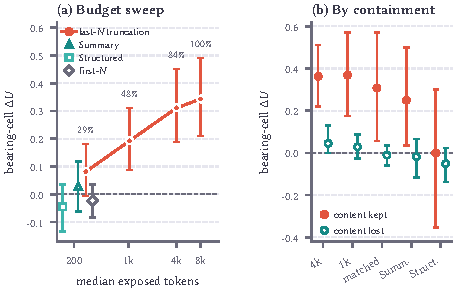
\includegraphics[width=\columnwidth]{fig_lenctl}
\caption{Length-control run on LongMemEval-V2: $\Delta U$ on the
$\lcBearCells$ bearing cells, task-clustered 95\% intervals.
\textbf{(a)}~Raw truncated to its last 4,096 and 1,024 tokens and to each
cell's Summary length (line), against Summary, Structured and the first-$N$
window at that length; percentages give the share of cells whose text still
contains the bearing content. \textbf{(b)}~The same arms split by whether
their text kept the bearing content (filled) or lost it (hollow).}
\label{fig:lenctl}
\Description{Left: bearing-cell utility rising with exposed tokens from about 0.08 at 280 tokens to 0.34 at 8,000, with Summary, Structured and first-N near zero. Right: for each arm, utility near 0.25 to 0.37 when the bearing content is kept and near zero when it is lost, except Structured whose kept estimate is near zero with a wide interval.}
\end{figure}

The length control was frozen before execution. Its extractive arm keeps the
final $N$ tokens of the same source segment, with $N$ set per cell to that
cell's own Summary token count, so it matches Summary's budget without any
model choosing content; a second arm keeps the first $N$ tokens instead, and
last-$N$ versus first-$N$ was registered as the decisive contrast. All three
pre-registered contrasts are computed on the $\lcBearCells$ bearing cells
(two replicate rows each, $\lcPrimaryN$ rows) and clustered over
$\lcBearTasks$ tasks: extractive versus Summary ($\lcPrimary$
$[\lcPrimaryLo, \lcPrimaryHi]$), Raw versus matched extractive ($\lcBudget$
$[\lcBudgetLo, \lcBudgetHi]$), and last-$N$ versus first-$N$ ($\lcEnds$
$[\lcEndsLo, \lcEndsHi]$).

The same run truncated Raw to its last 4,096, 1,024 and 20,000 tokens; the last
equals Raw, since no segment is longer. Table~\ref{tab:sweep} gives each arm's
bearing-cell $\Delta U$, its retention of the bearing content, and $\Delta U$
split by retention. \texttt{make\_lenctl.py} computes every entry from the row
file, whose checksum it verifies against the run manifest, and first checks
that it reproduces the three pre-registered contrasts. The run is not strictly
one session: $\lfLcCacheHits$ responses came from a cache filled minutes
earlier, and $\lcNullRows$ rows with a null reward are excluded, never zeroed.

\begin{table}[t]
\centering\footnotesize
\setlength{\tabcolsep}{2.4pt}
\caption{Length-control run on LongMemEval-V2: bearing-cell $\Delta U$ by arm
($\lcBearCells$ cells, task-clustered 95\% intervals), share of cells whose text
still contains the bearing content, and $\Delta U$ split by whether it does.
Exploratory beyond the three pre-registered contrasts.}
\label{tab:sweep}
\begin{tabular}{@{}lrrrrr@{}}
\toprule
arm & median tokens & kept & $\Delta U$ & $\Delta U\mid$kept & $\Delta U\mid$lost \\
\midrule
Raw (full) & \lcRawTok & \lcRawKept\% & \lcRawM\ [\lcRawLo, \lcRawHi] & \lcRawKM & -- \\
last 4,096 & \lcFourTok & \lcFourKept\% & \lcFourM\ [\lcFourLo, \lcFourHi] & \lcFourKM & \lcFourLM \\
last 1,024 & \lcOneTok & \lcOneKept\% & \lcOneM\ [\lcOneLo, \lcOneHi] & \lcOneKM & \lcOneLM \\
last $N$ (matched) & \lcMatchTok & \lcMatchKept\% & \lcMatchM\ [\lcMatchLo, \lcMatchHi] & \lcMatchKM & \lcMatchLM \\
Summary & \lcSumTok & \lcSumKept\% & \lcSumM\ [\lcSumLo, \lcSumHi] & \lcSumKM & \lcSumLM \\
Structured & \lcStrTok & \lcStrKept\% & \lcStrM\ [\lcStrLo, \lcStrHi] & \lcStrKM & \lcStrLM \\
first $N$ (matched) & \lcFirstTok & \lcFirstKept\% & \lcFirstM\ [\lcFirstLo, \lcFirstHi] & -- & \lcFirstLM \\
\bottomrule
\end{tabular}
\end{table}

\paragraph{Is the kept subset easier?} Retention is a property of the text,
fixed before any outcome, but the cells where a compressed text keeps the
content could still be easier ones. They are not for Summary or the matched
truncation: on the same cells, Raw gains $\lcSelSumKept$ where Summary kept the
content and $\lcSelSumLost$ where it lost it ($\lcSelMatchKept$ and
$\lcSelMatchLost$ for the matched truncation). For Structured the kept cells are
\emph{harder} ($\lcSelStrKept$ against $\lcSelStrLost$), which accounts for
its low kept estimate.

\paragraph{Position.} Target position is identical across all eight arms
within each cell (asserted). Between strata its distribution differs mildly
($\chi^2$ $p = \lcPosChiP$); the position-standardized Raw
\textsc{bearing}$-$control contrast is $\lcPosStd$ against $\lcPosUnadj$
unadjusted, and positive at every position.

\subsection{Formation-cost sensitivity}
\label{sec:reuse}
Formation cost per cell is the writer's tokens divided by the reuse factor
$r$, the number of cells that share one written memory. Our design fixes
$r = \frReuse$, so we recompute exposure efficiency over $r$ from the same
utilities and token counts (Figure~\ref{fig:reuse}). One Summary costs about
$\raFormSum$ writer tokens and one Structured record about $\raFormStr$. On
point estimates Summary overtakes Raw only for $r \gtrsim \raReuseStar$, but
its utility interval spans zero at every $r$, so the crossing point is not
estimated with any precision. Under the sparsity we measure, a memory that
bears on one task may be shown for few others, which pushes $r$ down and
formation cost up. The relevant factor in deployment is exposures per write,
not cells per memory. Input and output tokens are priced identically and prompt
caching is ignored; since output tokens usually cost more, both choices
understate the writer's cost.

\begin{figure}[t]
\centering
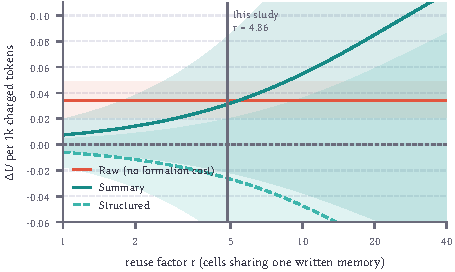
\includegraphics[width=\columnwidth]{fig_reuse}
\caption{Exposure efficiency ($\Delta U$ per thousand charged tokens) against
the reuse factor, on the $\frCells$ representation cells of LongMemEval-V2.
Lines use each representation's paired \textsc{bearing}$-$control effect;
bands use its 95\% interval over memories. Raw has no writer call and does not
depend on $r$. The vertical line marks the reuse factor of this study.}
\label{fig:reuse}
\Description{Line chart of efficiency against reuse factor on a log axis: Raw is flat near 0.034, Summary rises and crosses Raw near r of 5.5 with a wide band spanning zero, Structured is below zero.}
\end{figure}

\section{Second reader and writer, $\times$, reader factorial}
\label{sec:readerfull}

\paragraph{Design.}
The second-reader study was pre-registered before any design-cell call was
issued, with no transfer, the same ordering at a different magnitude, and a
different representation preference all committed as valid outcomes. The
memory file, prompt, filler pool, every rendered request, and each cell's
target position were hash-asserted against the first run at call time, and
the text re-verified byte-identical on $\rgRows$ rows; in the session-matched
run all $\smIdentK$ of $\smIdentN$ joinable rows are hash-identical.

\paragraph{Session-matched result.}
Both readers ran in one session. Over $\rgSmCells$ matched Raw cells on
$\rgSmTasks$ tasks ($\rgSmN$ replicate rows; these three counts are different
units), mean $\Delta U$ is $\rgSmOss$ under the first reader and $\rgSmGem$
under the second, a paired change of $\rgSmDiff$ $[\rgSmLo, \rgSmHi]$. The
two readers' own 95\% intervals overlap; plotting those would invite a ``no
difference'' reading that the paired design rules out. The within-memory
\textsc{bearing}$-$control contrast is $\rgBmcRawOss$ $[\rgBmcRawOssLo,
\rgBmcRawOssHi]$ under the first reader and $\rgBmcRawGem$ $[\rgBmcRawGemLo,
\rgBmcRawGemHi]$ under the second ($\rgBmcRawOssMem$ memories). The no-memory
arm moves by $\rgWithoutDelta$, so part of the gain is a weaker reader rather
than a better memory.

\paragraph{Cross-session first execution.}
A first execution with the two readers a day apart returned $\rgRawDiff$
$[\rgRawLo, \rgRawHi]$, inside the session-matched interval. Re-run together,
that difference splits into $-0.0327$ attributable to the session and
$-0.0364$ to the reader, which halves the apparent reader share. We quote only
the session-matched estimate.

\paragraph{Cell-level agreement, session-matched run.}
These are the numbers behind Figure~\ref{fig:overview}f. Over the
$\rgSmCells$ matched Raw cells, the readers' three-way labels (helped,
unchanged, hurt) agree on $\raReaderLabAgree$ of $\rgSmCells$ cells, at Cohen's
$\kappa = \raReaderKappa$; $\smCZeroZero$ cells are unchanged under both and
can only agree. Of the $\raReaderMoving$ cells that move under either reader,
both mark $\smAgree$ as helped, and signs agree on $\smAgree$ of the $\smBoth$
cells that move under both. The readers agree on no harmed cell (the first
reader's $\raHurtOss$ and the second's $\raHurtGem$ do not overlap), but so few cells
are harmed that this cannot show whether harm labels reproduce.

\paragraph{Cell-level agreement, earlier cross-session run.}
The first execution, with the two readers a day apart, covers a slightly
different matched set ($\rgRawN$ cells) and is the only source for Summary and
Structured. There the readers' per-cell $\Delta U$ correlate at
$r{=}\rgRawRAll$ over all cells, of which $\rgRawZeroBoth$ are zero under both;
over the $\rgRawNNz$ cells non-zero under either reader, $r = \rgRawRNz$
($\rgSumRNz$ for Summary, $\rgStrRNz$ for Structured). Signs agree on
$\rgRawSignK$ of $\rgRawSignN$ Raw cells where both move, and labels on
$\rgRawLabK$ of $\rgRawLabN$. Summary $\rgSumDiff$ $[\rgSumLo, \rgSumHi]$ and
Structured $\rgStrDiff$ $[\rgStrLo, \rgStrHi]$ span zero with only
$\rgSumNNz$ and $\rgStrNNz$ cells non-zero under either reader. Because this
run spans sessions, its numbers mix reader and session differences, and they
should not be pooled with the session-matched ones. Costs are not pooled
across readers: the second reports no reasoning-token counts.

\paragraph{Writer, $\times$, reader factorial.}
\label{sec:factorial}
All four writer--reader arms ran in one session. Every one of the eight
contrasts (writer, reader, same-family and interaction, on Summary with
$n{=}274$ and Structured with $n{=}268$) spans zero. The intervals are
informative rather than underpowered: they exclude writer and same-family
effects larger than $0.0380$, against the $\rgSmDiff$ reader effect the same
apparatus detects. Raw has no writer and is not in the factorial, and two
checkpoints form a $2\times2$ design, not a population of models.

\section{Cross-benchmark contrasts}
\label{sec:crossbenchtable}
The one quantity all three benchmarks define identically is the per-cell
representation contrast: a representation's $\Delta U$ minus Raw's on the same
memory and task. It separates from zero on LongMemEval-V2 alone
(Figure~\ref{fig:overview}e): Summary$-$Raw is $\xbSRLmM$
$[\xbSRLmLo, \xbSRLmHi]$ and Structured$-$Raw is $\xbTRLmM$
$[\xbTRLmLo, \xbTRLmHi]$ on $\xbSRLmN$ cells. On SciCode ($n{=}\xbSRScN$) and
SWE-bench Verified ($n{=}\xbSRSwN$) every interval includes zero, but there the
memories themselves have no effect even in raw form: Raw's own $\Delta U$ is
$\rvSciRaw$ $[\rvSciRawLo, \rvSciRawHi]$ on SciCode, where $\rvSciRawTied$ of
$\rvSciRawN$ cells are unchanged, and $\rvSweRaw$ $[\rvSweRawLo, \rvSweRawHi]$
on SWE-bench. With no Raw effect to preserve or lose, a representation contrast
there is uninformative about representation; these benchmarks bound where
memory matters for this reader, not how it should be written
(Section~\ref{sec:crossbenchtable}).

Table~\ref{tab:crossbench} gives the values plotted in
Figure~\ref{fig:overview}e. We compare contrasts rather than
per-representation $\Delta U$ because each benchmark carries its own
nondeterminism. The no-memory arm, whose input is identical across
representations, still disagrees with itself on
$\xbFloorLmK/\xbFloorLmN{=}\xbFloorLm$ of LongMemEval-V2 cells and
$\xbFloorScK/\xbFloorScN{=}\xbFloorSc$ of SciCode cells, and a paired contrast
removes that term. SWE-bench has no such floor because its no-memory arm is
deterministic by construction. SciCode's equivalent judge control disagrees
on 5 of 135 cells within one session, so determinism cannot be assumed of a
new benchmark.

\begin{table}[t]
\centering\footnotesize
\setlength{\tabcolsep}{4pt}
\caption{Per-cell representation contrasts: $\Delta U$ under one
representation minus $\Delta U$ under Raw on the same memory and task, with
task-clustered 95\% intervals. Only LongMemEval-V2 separates from zero. Every
SciCode and SWE-bench interval includes zero (SWE-bench's Summary$-$Raw only at
its upper bound), and doubling the SciCode cell
count separated no contrast. MDE is the minimum detectable contrast at 80\%
power and two-sided $\alpha = 0.05$, computed from each interval's width.
Raw's own with-versus-without $\Delta U$ is $\rvSciRaw$
$[\rvSciRawLo, \rvSciRawHi]$ on SciCode and $\rvSweRaw$ on SWE-bench, so on
these benchmarks no memory effect exists for a representation to preserve, and
the contrasts cannot test the ordering.}
\label{tab:crossbench}
\setlength{\tabcolsep}{3pt}
\begin{tabular}{@{}llrrrr@{}}
\toprule
contrast & benchmark & $n$ & mean & 95\% CI & MDE \\
\midrule
Summary$-$Raw
 & LongMemEval-V2 & \xbSRLmN & \xbSRLmM & [\xbSRLmLo, \xbSRLmHi] & \raMdeSRLm \\
 & SciCode        & \xbSRScN & \xbSRScM & [\xbSRScLo, \xbSRScHi] & \raMdeSRSc \\
 & SWE-bench      & \xbSRSwN & \xbSRSwM & [\xbSRSwLo, \xbSRSwHi] & \raMdeSRSw \\
\midrule
Structured$-$Raw
 & LongMemEval-V2 & \xbTRLmN & \xbTRLmM & [\xbTRLmLo, \xbTRLmHi] & \raMdeTRLm \\
 & SciCode        & \xbTRScN & \xbTRScM & [\xbTRScLo, \xbTRScHi] & \raMdeTRSc \\
 & SWE-bench      & \xbTRSwN & \xbTRSwM & [\xbTRSwLo, \xbTRSwHi] & \raMdeTRSw \\
\bottomrule
\end{tabular}
\end{table}

\section{Sign reversal and the decomposition}
\label{sec:negative}
\paragraph{Why flip rates cannot be compared across strata.}
A memory can show a flip only if at least two of its cells move with opposite
signs, so the chance of a flip grows with the number of cells per memory. In
the screened design a memory has $\raCellsPerMemBear$ \textsc{bearing} cells
and $\raCellsPerMemRand$ \textsc{random} cells on average. The naive
contrast (0 of 35 \textsc{bearing} memories against 17 of 60 \textsc{random},
Fisher one-sided $p = 1.5\times10^{-4}$) therefore mostly reflects that
difference. To test this, we took each of the $\raMatchedN$ memories with at
least two \textsc{bearing} cells and drew, without replacement, as many of its
\textsc{random} cells as it has \textsc{bearing} cells, then recounted flips
(20{,}000 resamples). The random stratum averages $\raMatchedMean$ flips and
shows none in $\raMatchedPZero\%$ of resamples (Figure~\ref{fig:reversal}b), so
0 of 35 is what chance alone would most often produce. A Wilson bound on the \textsc{bearing} flip rate would also treat 35 memories
from 21 episodes as independent.
Matching each memory's random subsample on the no-memory outcome as well (so
both strata get the same opportunities to help and to hurt) leaves all
$\lfCondFlipMems$ memories eligible; the random stratum then shows a mean of
$\lfCondFlipMean$ flips and none in $\lfCondFlipPZero\%$ of resamples. We
therefore do not compare flip rates across strata.

\paragraph{Why the sign of moving cells is not a comparison either.}
A tempting alternative compares the share of negative cells among cells that
move: $\raNegBearK$ of $\raNegBearN$ for \textsc{bearing} against
$\raNegRandK$ of $\raNegRandN$ for \textsc{random}. That comparison is
confounded by baseline accuracy. A memory can only hurt where the reader was
correct without it, and \textsc{bearing} tasks have the lowest no-memory
accuracy, so they offer the fewest chances to hurt.

\paragraph{Transitions conditioned on the no-memory outcome.}
Reward is binary in the screened run: each stratum's mean equals
(helped $-$ hurt)$/n$ exactly. With Table~\ref*{M-tab:screened}'s both-arms-fail
rate this fixes the full transition table (Table~\ref{tab:transitions}).
Conditioned on opportunity, the strata do not differ detectably in harm,
and they differ sharply in help (Figure~\ref{fig:reversal}a). In the
\textsc{random} stratum help and harm rates are close, the signature of a
content-independent response to inserting an item, which we treat as the
perturbation floor (\main{sec:metrics}). The table's Wilson intervals treat cells as
independent. Resampling memories instead, the harm rates have intervals of
$[\lfHurtClBearLo, \lfHurtClBearHi]$ (\textsc{bearing}),
$[\lfHurtClCtrlLo, \lfHurtClCtrlHi]$ (control) and
$[\lfHurtClRandLo, \lfHurtClRandHi]$ (\textsc{random}), which overlap, and the
help rates $[\lfHelpClBearLo, \lfHelpClBearHi]$,
$[\lfHelpClCtrlLo, \lfHelpClCtrlHi]$ and $[\lfHelpClRandLo, \lfHelpClRandHi]$,
where \textsc{bearing}'s is disjoint from the others. Both
analyses here are exploratory and are produced by
\texttt{make\_reanalysis.py}, which first checks that it reproduces every flip
count and stratum mean in the paper.

\begin{table}[t]
\centering\footnotesize
\setlength{\tabcolsep}{2.6pt}
\caption{Screened run on LongMemEval-V2: transitions between the no-memory
and with-memory outcome (binary reward). Accuracy columns give the share of
cells answered correctly without and with the memory. Hurt is conditioned on
cells correct without the memory, help on cells wrong without it; Wilson 95\%
intervals in brackets.}
\label{tab:transitions}
\begin{tabular}{@{}lrrrrr@{}}
\toprule
stratum & $n$ & acc.\ w/o & acc.\ with & hurt $\mid$ correct & help $\mid$ wrong \\
\midrule
\textsc{bearing} & \spBearN & \raAccZeroBear & \raAccOneBear
  & \raHurtRateBear\ [\raHurtLoBear, \raHurtHiBear] & \raHelpRateBear\ [\raHelpLoBear, \raHelpHiBear] \\
control & \spCtrlN & \raAccZeroCtrl & \raAccOneCtrl
  & \raHurtRateCtrl\ [\raHurtLoCtrl, \raHurtHiCtrl] & \raHelpRateCtrl\ [\raHelpLoCtrl, \raHelpHiCtrl] \\
\textsc{random} & \spRandN & \raAccZeroRand & \raAccOneRand
  & \raHurtRateRand\ [\raHurtLoRand, \raHurtHiRand] & \raHelpRateRand\ [\raHelpLoRand, \raHelpHiRand] \\
\midrule
\multicolumn{6}{@{}l}{\emph{opportunities:} hurt $\raHurtOppBear$ / $\raHurtOppCtrl$ / $\raHurtOppRand$ cells;
help $\raHelpOppBear$ / $\raHelpOppCtrl$ / $\raHelpOppRand$ cells} \\
\bottomrule
\end{tabular}
\end{table}

\paragraph{The additive-null comparison.}
Fitting $\mu + a_m + b_t$ and simulating from it, the excess of the observed
reversal rate over the fitted additive model is negative in all three strata.
Two independent implementations agree on the sign and disagree on the
magnitude, so we quote only the sign.

\paragraph{Why the decomposition is not identifiable.}
The within-session execution floor is exactly zero: replicates issued 0--16
seconds apart agree on 1{,}157 of 1{,}157 cells. With no residual scale, the
fitted residual collapses and the task and interaction shares are not
separately identified, so we report none. Clean per-cell utilities and a
variance decomposition are in tension on a reader without execution noise.

\begin{figure}[t]
\centering
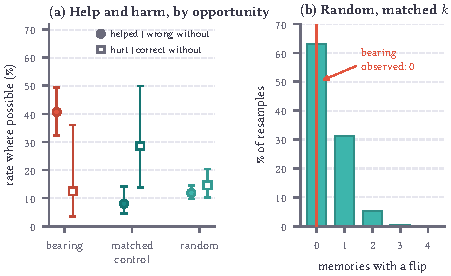
\includegraphics[width=\columnwidth]{fig_reversal}
\caption{Sign reversal on LongMemEval-V2, screened design (1{,}157 cells,
60 memories). \textbf{(a)}~Help rate among cells the reader got wrong without
the memory (filled) and harm rate among cells it got right (hollow), with
Wilson 95\% intervals; counts are in Table~\ref{tab:transitions}. Harm does not differ detectably across
strata; help does. \textbf{(b)}~Flips among the 35 memories with at least two
\textsc{bearing} cells when each memory's \textsc{random} cells are subsampled
to its own \textsc{bearing}-cell count (20{,}000 resamples); the line marks the
observed \textsc{bearing} count.}
\label{fig:reversal}
\Description{Left: dot plot of help and harm rates by stratum; help is about 41 percent for bearing against 8 and 12 percent elsewhere, harm overlaps across strata at 12 to 29 percent with wide intervals. Right: histogram of flip counts at matched cell counts, with zero flips in about 63 percent of resamples.}
\end{figure}

\section{Data, code and prompt availability}
\label{sec:repro}
\label{sec:prompts}
\paragraph{Public dataset.} The Conditional Memory Utility Dataset is available on
\href{https://huggingface.co/datasets/AgentsSci/AAMAS2027-ConditionalMemory}{Hugging Face}.
The frozen \texttt{v0.6-}\allowbreak\texttt{length-control} snapshot contains 16,816 records:
16,535 from LongMemEval-V2, 154 from SciCode, and 127 from SWE-bench Verified.
A row describes a memory--task pair under a representation, reader, condition
and replicate, with the outcome under each arm, available output text and
cost metadata. Missing or unscorable measurements remain explicitly marked;
they must not be converted to zero rewards.

\paragraph{Version and reproducibility.} The data file is
\texttt{data/}\allowbreak\texttt{cells.jsonl}. The repository also provides a manifest with file checksums, schema and validation
code, and documentation of the included conditions and upstream sources.
Readers can download the data directly or pin the
\texttt{v0.6-}\allowbreak\texttt{length-control} revision with the Hugging Face client. The data
card contains a runnable download example and explains the validation warnings.
This snapshot was built on 2 October 2026 and does not contain every later
manuscript analysis; in particular, its condition inventory does not include
the fixed-total-context experiment. The public Hub package contains schema and
validation code, not the complete experiment, analysis and prompt bundle.
The length-control identity arm is an A/A control and must not be pooled with
Raw as an independent condition. Per-pair utility labels describe the recorded
evaluation conditions, rather than unconditional training targets.

\paragraph{Withheld and missing text.} The 154 SciCode records contain Raw
memories; their reader outputs were not retained. SciCode Summary and Structured
records are absent because their memory text was not persisted. The 127
SWE-bench records provide identifiers and derived measurements, with restricted
corpus and output text withheld under the release policy. These are distinct
from records missing because of a persistence gap. The data card documents the
sentinels and per-source reuse terms; access to the dataset does not grant a
new license to withheld upstream content.

\section{Extended limitations}
\label{sec:extlimits}

\paragraph{Leakage rates are lower bounds.}
Our leakage detector reuses the benchmark's phrase matcher, whose normalizer
strips punctuation without inserting a space. A gold phrase next to a quote
or an equals sign is glued to its neighbor and the match fails. Such leaks
are missed, and punctuation is common in accessibility trees, so every
leakage rate we report is a lower bound. A control test records the defect, so
an upstream fix would be detected. The 156
LLM-judged questions cannot be audited without an inference call and are
recorded as undecidable rather than clean. 69 multiple-choice questions with
gold answers of one to five characters cannot be audited structurally and are
never folded into a pooled rate.

\paragraph{The judge floor measures decoding.}
$F_{\mathrm{judge}}$ is zero wherever we measured it: over $\lfJudgeObs$
explicit re-scorings of $\lfJudgeUnits$ units in the earlier official arm, and
in every stratum of the screened run. Both estimators carry a positive control
(a planted disagreement makes them fire). A zero floor here reflects a
deterministic scorer and greedy decoding, not an unambiguous rubric. The
SciCode control in Section~\ref{sec:crossbenchtable}, which disagrees on 5 of
135 cells, is a different scorer on a different benchmark. We have no
cross-session floor for any arm and presume it to be non-zero.
%%% NOTE: earlier drafts quoted "240 of 240" and "288 re-scorings"; neither
%%% figure could be traced to a ledger in results/, so both were replaced.

\paragraph{Semantic type.}
We intended semantic memory type as a second axis, but in our representation
pilot the two labeling passes agreed on 3 of 8 segments at Cohen's
$\kappa = 0.000$: the structured writer's own pass called every segment
\texttt{episodic}, a degenerate marginal, so we report no semantic-type
breakdown. Separately, exactly one deterministically scorable
\emph{errors-gotchas} question exists in the benchmark and accounts for 865 of
6{,}920 web cells, so any per-stratum result there is a single-question result.

\paragraph{Writer failures and faithfulness.}
The structured writer failed on 3 of 60 segments, all by exhausting the token
budget mid-value rather than by malformed output, and on 0 of the 57 writes
that finished. An 8-segment pilot had put the failure rate at 0 of 8 and could
not have seen this, since it never reached the cap. Our faithfulness measures
are a screen, not a guarantee: a low score is strong evidence of a problem,
a high score is weak evidence of its absence, and they do not detect
recombination, omission, unsupported inference or negation.

\paragraph{Unrecorded quantities.}
Two quantities were not recorded during the runs and cannot be recovered: how
many gold-free picks contain the answer, and how the 12 position-probe cells
were chosen, which is why we treat that probe as a pilot.

\paragraph{Stated exclusions.}
17 of the 295 deterministically scored questions have no memory unit that
carries their gold answer under the segmentation answerability check, so their
cells can only yield $\Delta U \le 0$. The bearing screen, a looser containment
test, fires on no unit for $\soScrZero$ of them (Section~\ref{sec:sophia}).
23 of the 1{,}889 units (1.2\%) are their entire trajectory.

\section{Pre-registration record}
\label{sec:prereg}
Each pre-registered analysis was fixed in a pre-commitment document in the code
repository before the data it governs existed. The documents are released with
the code. To preserve anonymity we omit their commit identifiers here; the
release links each one to a commit and its timestamp, so its timing can be
checked on de-anonymization. Table~\ref{tab:prereg} lists every pre-registered analysis, its
anchor, and every deviation the run ledgers record. Pre-commitments were not edited after
the fact; where a result does not match one, the mismatch is reported.

\begin{table}[h]
\centering\footnotesize
\setlength{\tabcolsep}{3pt}
\caption{Pre-registered analyses, their anchors, and recorded deviations.}
\label{tab:prereg}
\begin{tabular}{@{}p{0.27\columnwidth}p{0.30\columnwidth}p{0.37\columnwidth}@{}}
\toprule
analysis & anchor & recorded deviation \\
\midrule
screened design and its reduction criterion & criterion fixed in code before the numbers existed & none recorded \\
reversal rate (headline) & pre-registration, section~5 & comparison with an additive null added later, as a diagnostic \\
variance decomposition & pre-registration, section~6 & not identifiable here (zero execution floor); in earlier arms the mixed model did not converge and the registered fallback was used \\
gold-free screens & gold-free screen pre-commitment & none recorded \\
length control & frozen at a recorded commit, before execution & \lfPrLcMismatch\ of \lfPrLcCompared\ descriptive figures do not re-derive: bearing quartile means by Raw length; none appears in the paper \\
second reader & written before any design-cell call & cross-session estimate superseded by a session-matched run \\
session-matched reader run & falsifiers committed before data & none recorded \\
writer\,$\times$\,reader factorial & factorial pre-commitment & one prose sign error ($-\tfrac12$ for $+\tfrac12$ interaction); replication check fails on sign only \\
SciCode scale-up & scale-up pre-commitment & none recorded \\
\bottomrule
\end{tabular}
\end{table}

\paragraph{The two deviations that bear on results.} The additive-null
comparison of reversal rates (\main{sec:r0}) was \emph{not} pre-registered;
the registered headline is the reversal rate itself, and the comparison is a
diagnostic added afterwards. In the writer\,$\times$\,reader factorial, the
registered criterion asked the re-measured reader effect to reproduce the
earlier one in sign and significance. Both estimates are near zero and span
zero (Summary $\lfPrWfSumOld$ then $\lfPrWfSumNew$, Structured
$\lfPrWfStrOld$ then $\lfPrWfStrNew$), so the significance verdict reproduces
and the sign does not; the two intervals contain each other's point estimates.
The factorial's pre-commitment also states that the same-family effect equals
$-\tfrac12$ of the interaction; the correct relation, which the analysis code
checks numerically, is $+\tfrac12$. Every quantity was computed as registered.

\section{Follow-up runs}
\label{sec:sophia}
Three follow-up runs test the main results under conditions the main design
held fixed; all are exploratory and used the same serving endpoint and reader as
the main runs. A generator script in the released code computes every number
below from the row files.

\paragraph{Second session, randomized position.} All $\soXoneCells$ bearing and
control cells, three replicates each, the memory's position redrawn per
replicate ($\soXoneCalls$ real calls, $\soXoneCacheHits$ from cache,
$\soXoneErr$ failed and excluded). Bearing minus control, paired within memory:
$\soXoneD$ $[\soXoneLo, \soXoneHi]$ over $\soXoneMems$ memories;
episode-clustered $[\soXoneEpLo, \soXoneEpHi]$ ($\soXoneEps$ episodes); two-way
(memory $\times$ task) $\soXoneTw$ $[\soXoneTwLo, \soXoneTwHi]$. Across the
three positions of a cell, the label changes in $\soPosChg$ of $\soPosCells$
cells ($\soPosChgPct\%$), and in $\soPosChgMv$ of the $\soPosMov$ cells that move
at least once ($\soPosChgMvPct\%$); position accounts for $\soPosVarPct\%$ of
the variance of $\Delta U$. Joined one-to-one to the published run, labels agree
in $\soStabSamePct\%$ of $\soStabSameN$ replicate-cells at the same position
($\kappa = \soStabSameK$) and in $\soStabDiffPct\%$ of $\soStabDiffN$ at a new
one ($\kappa = \soStabDiffK$).

\paragraph{Fixed total context.} $\soXtwoCells$ cells over $\soXtwoMems$
memories, two replicates. For each cell, $T$ is the base filler plus the Raw
memory; every other arm, and the no-memory arm, is padded after the base context
with bearing-disjoint filler to $T$ (asserted equal across arms), the memory
kept at its K2 position. \emph{Disclosed defect:} the no-memory cache key was
(trajectory, task, replicate), so two memories from one trajectory paired with
one task could share a no-memory response although their padding differs. The
headline numbers exclude all $\soXtwoCollCells$ such cells ($n=\soFN$ bearing
cells); including them ($n=\soFNAll$) changes no conclusion:

\begin{table}[!ht]
\centering\footnotesize
\setlength{\tabcolsep}{3pt}
\caption{Bearing-cell $\Delta U$ at a fixed total context (task-clustered
95\% intervals).}
\label{tab:fixedctx}
\begin{tabular}{@{}lll@{}}
\toprule
arm & excluding exposed cells & all cells \\
\midrule
Raw & \soFRaw\ [\soFRawLo, \soFRawHi] & \soFRawAll\ [\soFRawAllLo, \soFRawAllHi] \\
Summary & \soFSum\ [\soFSumLo, \soFSumHi] & \soFSumAll\ [\soFSumAllLo, \soFSumAllHi] \\
Structured & \soFStr\ [\soFStrLo, \soFStrHi] & \soFStrAll\ [\soFStrAllLo, \soFStrAllHi] \\
matched truncation & \soFTr\ [\soFTrLo, \soFTrHi] & \soFTrAll\ [\soFTrAllLo, \soFTrAllHi] \\
Summary $-$ Raw & \soFSumR\ [\soFSumRLo, \soFSumRHi] & \soFSumRAll\ [\soFSumRAllLo, \soFSumRAllHi] \\
Structured $-$ Raw & \soFStrR\ [\soFStrRLo, \soFStrRHi] & \soFStrRAll\ [\soFStrRAllLo, \soFStrRAllHi] \\
\bottomrule
\end{tabular}
\end{table}

The matched truncation is sensitive to the exclusion and supports no claim. The
cache key now includes the memory, so a re-run cannot repeat the defect.

\paragraph{Retrieval.} The reference labels are the screened design's (75 tasks, 266
bearing edges, reproduced and asserted). Each method ranks the task's whole
domain pool by the raw question; dense retrieval embeds 512-token chunks (a
unit scores its best chunk) or the first 2{,}000 tokens.

\begin{table}[!ht]
\centering\footnotesize
\setlength{\tabcolsep}{3pt}
\caption{Retrieval of bearing units (task-clustered 95\% intervals; chance
recall@10 is about \soChanceTenP). MRR is the mean reciprocal rank of the first
bearing unit; AUROC is the area under the ROC curve over bearing and
non-bearing units.}
\label{tab:retrieval}
\begin{tabular}{@{}lllll@{}}
\toprule
method & recall@1 & recall@10 & MRR & AUROC \\
\midrule
BM25 & \soRBmOne & \soRBmTen\ [\soRBmTenLo, \soRBmTenHi] & \soRBmMrr & \soRBmAuc \\
dense, prefix & \soRPreOne & \soRPreTen\ [\soRPreTenLo, \soRPreTenHi] & \soRPreMrr & \soRPreAuc \\
dense, chunks & \soRChkOne & \soRChkTen\ [\soRChkTenLo, \soRChkTenHi] & \soRChkMrr & \soRChkAuc \\
\bottomrule
\end{tabular}
\end{table}

Of the 295 deterministic questions, $\soScrZero$ fire on no unit, $\soScrDisc$
on one to eight, and $\soScrOver$ on more than eight. Without the cap, string
containment fires for all $\soNoCapMems$ memories, on $\soNoCapMin$ to
$\soNoCapMax$ tasks each.

\paragraph{Variance decomposition.} In the second-session run each cell has three
replicates at redrawn positions, which supplies the residual scale the main run
lacked. On the $\rvDecCells$ cells with all three replicates we fit the additive
model $\mu + a_m + b_t$ to cell means by least squares; its residual mean square
($\rvDecDf$ degrees of freedom) estimates the interaction variance plus the
within-cell variance divided by three, and the within-cell variance estimates the
residual. The shares are $\rvIntShare\%$ interaction, $\rvAddShare\%$ additive
memory and task effects, and $\rvEpsShare\%$ position with decoding; the
interaction $F$ test gives $F=\rvIntF$ ($p\rvIntP$). This is a method-of-moments
estimate on a sparse crossed design, reported as exploratory.

\paragraph{Power for harm.} With $16$ bearing cells able to show harm, against
the random stratum's rate of $\rvHarmRandPct\%$, the screened design detects
(80\% power, two-sided $\alpha=0.05$) only a bearing harm rate of
$\rvHarmMdePct\%$ or more; the null on harm is therefore weak evidence.

\paragraph{Containment inside the random-task stratum.} Memories in this stratum are real
same-domain pages. On the $\rvRandFireN$ random cells where the containment
detector fires (at any breadth) the memory helps in $\rvRandFireHelp\%$ of the
$\rvRandFireHelpN$ cells the reader got wrong without it, against
$\rvRandSilentHelp\%$ of $\rvRandSilentHelpN$ where it is silent; harm is
$\rvRandFireHurt\%$ and $\rvRandSilentHurt\%$. Part of the random stratum's help
is content, so its help rate bounds pure perturbation from above.

\paragraph{The gold-free screen over the full universe.} The model-based screen
was applied to all $\rvGfUniverse$ (task, unit) pairs: an exhaustive lexical
stage kept $\rvGfCand$ candidates, and the judge confirmed $\rvGfYes$ over
$\rvGfTasks$ tasks and $\rvGfMems$ memories, under the same cap of eight units
per task. A gold-free definition does not make bearing denser.

\paragraph{Sparsity across screen caps.} Recomputing the screen over the
deterministic tasks at four caps on the number of units a task may fire on:
at a cap of 4, $\rvCapFourTasks$ tasks and $\rvCapFourMems$ bearing memories;
at 8 (the paper's screen), $\rvCapEightTasks$ and $\rvCapEightMems$; at 16,
$\rvCapSixteenTasks$ and $\rvCapSixteenMems$; at 32, $\rvCapThirtyTwoTasks$ and
$\rvCapThirtyTwoMems$. At every cap the median bearing memory bears on exactly one
task, and $\rvCapShareLo$--$\rvCapShareHi\%$ bear on exactly one. Only removing the
cap entirely makes containment fire for every memory.

\paragraph{Which memories were sampled.} The 60 memories are every memory that
bears on two or more tasks and passes the size cap ($\rvSelMulti$ of the
corpus's $\rvPopMulti$) plus $\rvSelSingle$ single-task memories. The headline
contrast is $\rvHeadSingle$ $[\rvHeadSingleLo, \rvHeadSingleHi]$ on the
single-task memories and $\rvHeadMulti$ $[\rvHeadMultiLo, \rvHeadMultiHi]$ on the
multi-task ones; reweighted to the $\rvPopAll$ bearing memories of the corpus, of
which $\rvPopSinglePct\%$ bear on one task, it is $\rvHeadW$
$[\rvHeadWLo, \rvHeadWHi]$ (memory bootstrap within each group).


\section{Additional figures}
\label{sec:figs}
Figure~\ref{fig:overview} collects views referenced from the main paper: bearing
breadth, helped cells by stratum, retrieval, the representation contrasts with
their token costs, the cross-benchmark contrasts, and the two readers'
agreement. Figure~\ref{fig:lenctl} (Section~\ref{sec:lengthcontrol}) details the
length-control run.



\begin{figure*}[p]
\centering
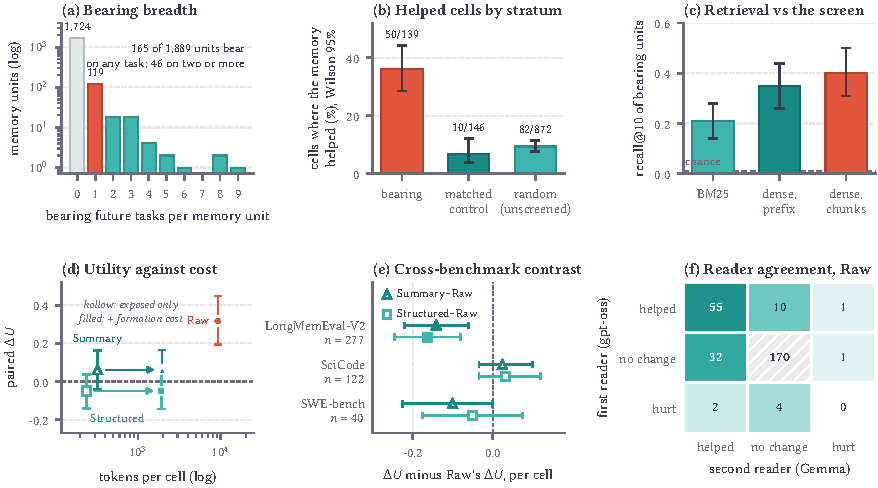
\includegraphics[width=\textwidth]{fig_results}
\caption{Overview of further results on LongMemEval-V2 (a--d, f) and across
benchmarks (e). \textbf{(a)}~Future tasks each of the $\bearUnits$ memory units
bears on, over $\bearDetTasks$ discriminative tasks (log axis).
\textbf{(b)}~Share of cells where the memory helped, cell-level Wilson 95\%
intervals (memory-resampled ones in Section~\ref{sec:negative}), for
the same $\spMems$ memories in three strata. \textbf{(c)}~Share of bearing units a retriever ranks in its top ten of the
domain pool (75 tasks, task-clustered 95\% intervals); the dashed line is
chance. \textbf{(d)}~Paired
\textsc{bearing}$-$control effect per representation ($\frCells$ cells,
$\frMems$ memories, intervals over memories); hollow markers count exposed
tokens, filled ones add formation cost amortized over $\frReuse$ cells.
\textbf{(e)}~Per-cell $\Delta U$ minus Raw's, task-clustered intervals; filled
markers exclude zero. \textbf{(f)}~Two readers' labels on $\rgSmCells$ Raw cells
in one session; the hatched cell (zero under both) cannot disagree.}
\label{fig:overview}
\Description{Six panels: a log histogram of bearing tasks per memory unit peaking at one; bar chart of helped-cell rates by stratum with bearing highest; similarity sextile lines nearly flat; utility against tokens showing Raw above zero and compressed representations near zero; cross-benchmark contrast intervals, only LongMemEval-V2 excluding zero; a three by three reader agreement table.}
\end{figure*}



